%\UseRawInputEncoding
\RequirePackage[l2tabu, orthodox]{nag}

\documentclass[12pt]{report}

\usepackage{amsmath}
\usepackage[a4paper,top=2.3cm,bottom=2.3cm,includeheadfoot]{geometry}
\usepackage{graphicx}
\usepackage[onehalfspacing]{setspace}
\usepackage{microtype} %use after fonts
\usepackage{siunitx}
%\usepackage{booktabs}
\usepackage{lastpage}
\usepackage{subcaption}
\usepackage{epigraph} % this is to add quotes at the beginning of chapters
\usepackage{bibunits}

\usepackage[colorinlistoftodos]{todonotes}
\usepackage{color}
\newcommand{\EliasComm}[1]{\todo[inline,color=blue!40]{EG: #1}}

%\DeclareUnicodeCharacter{00A0}{ }
%\DeclareUnicodeCharacter{00A0}{~}
%\DeclareUnicodeCharacter{2212}{-}
%\DeclareUnicodeCharacter{2010}{-}
%\DeclareUnicodeCharacter{2009}{\,} 
%\DeclareUnicodeCharacter{308}{"}


\usepackage{cite}
\usepackage[font={it}]{caption} % package to customise caption fonts
\usepackage[nottoc,numbib]{tocbibind} % This is to enable titles for table of contents, references etc.
\setlength{\headheight}{1.1\baselineskip}
\usepackage[automark]{scrlayer-scrpage} % package to customise the headers and footers
\pagestyle{scrheadings}
\clearscrheadfoot

\usepackage[final]{feynmp}
\DeclareGraphicsRule{*}{mps}{*}{}
\makeatletter
\def\endfmffile{%
	\fmfcmd{\p@rcent\space the end.^^J%
			end.^^J%
			endinput;}%
	\if@fmfio
		\immediate\closeout\@outfmf
	\fi
	\ifnum\pdfshellescape=\@ne
		\immediate\write18{mpost \thefmffile}%
	\fi}
\makeatother


\ofoot{\pagemark}
\ohead{\headmark}

\usepackage[colorlinks=true, citecolor=blue, linkcolor = black, pdfborder={0 0 0},backref=page]{hyperref}
\usepackage{cleveref}

\renewcommand*{\backref}[1]{}
\renewcommand*{\backrefalt}[4]{%
    \ifcase #1 (Not cited.)%
    \or        (Cited on page~#2.)%
    \else      (Cited on pages~#2.)%
    \fi}

\numberwithin{equation}{section}


\graphicspath{{pics/}{pics/Ch1_Introduction/}{pics/Ch2_Theory/}{pics/Ch3_Methods/}{pics/Ch4_Results1/}{pics/Ch5_Results2/}{pics/Ch6_Results3/}}

\begin{document}

\begin{titlepage}
\vspace*{\fill}
\begin{center}
\huge{Probing high-field QED effects with laser wakefield acceleration}\\[2cm]%\\[3.5cm]

\begin{figure}[ht]
\centering
\includegraphics[width=0.6\columnwidth]{Imperial_2_Pantones}
\end{figure}

\vspace{1.5cm}
\Large{Elias Gerstmayr}\\[1.0cm]%\\[3.5cm]
\large{\today}
\vfill
\normalsize{Submitted in partial fulfilment of the requirements for the degree of Doctor of Philosophy in Physics of Imperial College London and for the Diploma of Imperial College London.}
\vfill
\large{Department of Physics\\Imperial College London\\ Prince Consort Road\\ London SW7 2AZ}
\vfill
\end{center}
\end{titlepage}
\stepcounter{page}




\chapter*{Declaration}
\vspace*{\fill}

\newpage


\thispagestyle{plain}
%\maketitle
\vspace*{\fill}
\begin{center}

\textit{Da\ss \,\,ich erkenne, was die Welt}

\textit{Im Innersten zusammenh\"alt.}
\vspace{\baselineskip}

\textit{So that I may perceive whatever holds}

\textit{the world together in its inmost folds.}
\vspace{\baselineskip}

Johann Wolfgang von Goethe -- Faust. Der Trag\"odie erster Teil.
\vspace*{\fill}

\end{center}
\newpage

\thispagestyle{plain}

\vspace*{\fill}

\chapter*{Abstract}

The report is submitted to partially satisfy the requirements for the degree of Doctor of Philosophy (PhD). It begins with an overview and summary of experimental methods and theory relevant to the author's research, followed by an analysis of experimental data taken during the course of this degree.
The main focus of this thesis is using relativistic particles accelerated by laser wakefield acceleration and highly energetic radiation.

The first results presented are based on two recent colliding pulse experiment performed using the dual 300 TW Astra Gemini laser facility at the Rutherford Appleton Laboratory, where GeV scale electrons were collided with a high intensity laser beam to look for signatures of a fundamental process called radiation reaction.
Experimental evidence strongly indicates that the electron bunch and the laser beam were successfully overlapped in time and space at the collision point. Furthermore, results suggest that this happened at high laser intensities ($a_0 \sim 7$) and electron energies ($\sim 600\, \mathrm{MeV}$), generating radiation from inverse Compton scattering at photon energies of several tens of MeV, which is significantly higher than reported in previous experiments \cite{Sarri2014,Chen2013a,TaPhuoc2012a,Khrennikov2015}.

The second part of the results will be focused on a improved colliding pulse experiment, build upon the lessons learnt on the campaigns described in the first part.

The third chapter looks at another campaign performed at the Astra Gemini laser facility, this time attempting to generate matter from light through the simplest QED mechanism there is: the linear Breit-Wheeler process.
\vspace*{\fill}


\chapter*{Role of the Author}

Something about experiments and large teams and collaborations. Work in experimental groups for 9-12 experimental campaigns, mainly at Astra Gemini. Leading experiments as Target Area Operator, planning and design. Sometimes just one diagnostic.

The author has mainly been involved at experimental campaigns at the Astra Gemini laser facility at the Central Laser Facility (CLF), Rutherford Appleton Laboratory (RAL), Oxfordshire, UK. At the submission of this thesis, the author completed 10 campaigns in different roles, initially mainly setting up diagnostics of different kind, later on leading as Target Area Operator.

The results presented in chapter X are based on data taken on an experimental campaign at Gemini in 2015, during the first year of the author's PhD, investigating radiation reaction in the collision of a highly relativistic electron beam with a very intense laser pulse. During the campaign the author helped setting up different diagnostics and was mainly in charge of the electron spectrometer. Following the completion of the campaign the author analysed the electron spectra, their energy, shape and statistical stability. The author also processed data from a diagnostic measuring the gamma-ray spectrum and investigated links between the gamma-ray signal and electron spectra. This analysis was a crucial contribution to identify successful collisions of electron beam and laser pulse, and express statistical confidence in those results. The findings of this campaign were published in Cole et al., PRX 8 (2018), with the author of this thesis as third author. In this context another experiment was performed at the Astra Gemini facility. The results were published in Poder et al., PRX 8 (2018), with the author of this thesis as co-author.

In chapter X, the author presents results from another experimental campaign performed at the Astra Gemini laser facility on the topic of radiation reaction. The author was leading the planning efforts of this experiment over the course of several months and also took the lead of the  experimental execution in late 2018 until early 2019 as Target Area Operator (TAO).

In chapter X, the author presents results from an experimental campaign on the measurement of the linear Breit-Wheeler process. The author was strongly involved in the planning of this experiment and acted as Target Area Operator (TAO) for the time of the experiment. 

%\begin{center}
%\textbf{Publications}
%\end{center}

\iffalse
\chapter*{Publications}

The following publications contain work presented in this thesis:
\vspace{\baselineskip}
Special Issue ElecStability (this year to submit?), results from RR2? (realistically not before submission)

The author contributed to the following publications during the course of his PhD:

Cole RR PRX, Poder RR PRX, Keegan Gamma KSI, Amina imaging (soon to be submitted), Brendan XANES (soon to be submitted), Savio Cluster paper (soon to be submitted?), CP Ridgers special issue (soon to be submitted?), Joel chirp? (soon to be submitted), Roman SPIE special issue (soon to be submitted?), any imaging stuff?

% bibunit to list our publications
\begin{bibunit}
\renewcommand{\bibsection}{}%{\large \textbf{\begin{center}
%Publications
%\end{center}}}
\makeatletter
\renewcommand\@biblabel[1]{#1.}
\makeatother
\def\bibfont{\small}
 
%list all the references in the publications bibtex file
\nocite{*}
\putbib[mypub]
\end{bibunit}

\vspace*{\fill}
\fi

\newpage

\tableofcontents
\newpage

%
\chapter{Introduction}

\section{Particle Accelerators}

The advent of particle accelerators unveiled fundamental physics, new particles and processes. More energy to probe smaller and more fundamental particles and interactions.

\subsection{Conventional Accelerators}

\subsection{Plasma-based Accelerators}


\EliasComm{Plots to show energy versus year, energy spread and type of injection and whether it holds to the scaling laws.}

\section{Light Sources}

\subsection{Conventional Light Sources (Gen)}

Particle accelerators are traditionally also the source of bright radiation.

Laser wakefield accelerators are the source of a variable and tunable radiation source covering the few keV to 100 MeV range.
Wakefields are producing hard X-ray radiation through betatron radiation.
Through hosing or amplification of oscillations the radiation can reach the MeV range.
A second beam or backreflected can be used to weakly produce linear inverse Compton scattering in the tens to twenty MeV range.
In the nonlinear highly intense regime radiation to 40 or more MeV is possible.
They also are able to produce bremsstrahlung when dumped.

Source size, time duration are unique properties.

\EliasComm{How about a plot showing the capability of energies on a plot versus synchrotron sources.}

High energy radiation sources are rare on earth. Typically found in astrophysical phenomena, where these kinds of processes are more dominant as well. Inverse Compton scattering is a common sight there. Hard radiation in wakefields can be produced from several sources. Betatron radiation through amplified oscillation, bremsstrahlung, inverse Compton scattering, nonlinear inverse Compton scattering. Also several applications from imaging hard materials, nuclear processes, QED processes will require a diagnostics applicable over a whole bandwidth. New QED experiments reaching hundreds of MeV gamma radiation will have to rely on a shape-independent diagnostics and we have shown that this is necessary to distinguish models. Higher energy accelerators facilities will generate harder radiation as well and need to diagnose it.


Light sources are synchrotrons, large scale particle accelerators. KeV X-rays can be produced from relatively compact X-ray tubes.

Diagnostics:
Absorption X-rays
X-rays via filter packs, K-edges, crystals
converter targets and spectral measurement
differentially damped spectrum

\section{High field interactions and QED}

Radiation Reaction, Breit-Wheeler


\section{Thesis Outline}

Following this introduction the author will introduce some theoretical concepts and experimental methods relevant to this work.

2. theory
3. Experimental Methods 
4. some simulation stuff used in most of the results chapters


Results Chapters: High energy radiation from wakefield accelerators and their application

\begin{enumerate}
\setcounter{enumi}{4}
\item \textbf{Hard Betatron Radiation from dual shock structure} Electrons travelling in a wakefield transitioning through two density spikes experienced an increase of transverse oscillations resulting in an enhancement of measured betatron radiation. The dual shock structure was induced by introducing a blade into the supersonic gas flow of a helium gas jet. This radiation source could be used to image high-Z materials that can not be penetrated by standard betatron radiation. At the same time this opens up the possibility to explore this regime further and increase the brightness of the source even further.
\item \textbf{linear Inverse Compton Scattering} Electrons from a wakefield accelerator were collided with a strongly defocused laser pulse generating gamma radiation from linear inverse Compton Scattering. (and development of dual-axis gamma spectrometer)
\item \textbf{Nonlinear Inverse Compton Scattering and Radiation Reaction} By scattering a tightly focused high intensity laser pulse from a relativistic electron beam and generating gamma radiation from nonlinear Inverse Compton Scattering, it was possible to measure radiation reaction in an experiment. (as gateway to measuring and diagnosing radiation reaction)
\item \textbf{Linear Breit-Wheeler Process and Bremsstrahlung source} A dual laser setup is used to produce a thermal X-ray source and a gamma beam from bremsstrahlung in an attempt to measure the elusive linear Breit-Wheeler process. (or using a wakefield-based Bremsstrahlung source and a laser-solid interaction X-ray source to measure linear BW)
\end{enumerate}

\EliasComm{Put a plot of the photon energy ranges illuminated in the different result sections.}

\chapter{Theory}
\label{Chap:Theory}

This Chapter lays the theoretical groundwork for the results presented later in this work, addressing laser wakefield acceleration, radiation production from charged particles and the fundamental processes of radiation reaction and pair production.

Firstly, equation of motions of charged single particles in electromagnetic fields are derived. This forms the basis for understanding the properties of electrons accelerated in wakefield accelerators, measuring their energy in magnetic spectrometers and calculating the radiation they emit in interaction with electromagnetic fields.

Secondly, the propagation of a laser in a plasma and its non-linear evolution are discussed. This paves the way for the third section on laser wakefield acceleration where basic properties like maximum energy and injection mechanisms are introduced.

Subsequently, radiation production from electrons in different scenarios is discussed, starting with radiation in synchrotrons and insertion devices, then drawing the parallel to betatron radiation produced in wakefield acceleration and the radiation emitted in a laser wiggler, namely relativistic inverse Compton scattering (ICS) in moderately (linear ICS) and highly intense laser fields (non-linear ICS). Bremsstrahlung as radiation mechanism is also being introduced.

This leads over to the topic of radiation reaction, the knock-back force a charged particle experiences when emitting a photon. This can, for instance, be investigated in relativistic inverse Compton scattering. Whilst radiation reaction is a very fundamental phenomenon there is so far no universally accepted and practicable description for a wide parameter space. In this section different proposed descriptions of radiation reaction are discussed, starting with the in classical electrodynamics self-consistent Lorentz-Abraham-Dirac equation, followed by the classical Landau-Lifschitz equation and leading over to quantum corrections and their implications. 

Finally, other fundamental QED processes such as pair production, annihilation and light-light scattering is discussed.

\EliasComm{Once full structure is clear, revise this.}

\section{Single particle motion in an EM field}

The Lagrangian for a relativistic particle in an electromagnetic field with the potentials $\Phi$ and $\mathbf{A}$ is given by \cite{Jackson}
\begin{equation}
L(\mathbf{r},\mathbf{v},t) = - mc^2 \gamma^{-1}+q \mathbf{v}\cdot\mathbf{A} - q \Phi,
\end{equation}
where $m$ is the mass of the particle, $\gamma$ the relativistic Lorentz factor and $q$ the charge.
To obtain the equation of motion (EoM) we use the Euler-Lagrange equation
\begin{equation}
\frac{\mathrm{d}}{\mathrm{d}t} \frac{\partial L}{\partial \mathbf{v}} - \frac{\partial L}{\partial \mathbf{r}} = 0.
\end{equation}

Using $\mathbf{A} = \mathbf{A}(\mathbf{r},t)$, $\Phi = \Phi(\mathbf{r},t)$, $\gamma^{-1} = \sqrt{1-(v/c)^2}$ and this becomes
\begin{equation}
\frac{\mathrm{d}}{\mathrm{d}t} \left[\mathbf{p}+q\mathbf{A}\right]-\left[q\nabla\left( \mathbf{A} \cdot \mathbf{v}\right) - q\nabla \Phi \right] = 0,
\label{Theory:Eqns:EoMLorentzRaw}
\end{equation}
where $\mathbf{p} = \gamma m \mathbf{v}$ is the relativistic momentum.
Now using $\frac{\mathrm{d}}{\mathrm{d}t} = \frac{\partial}{\partial t} + \mathbf{v} \cdot \nabla$ and the vector identity $\nabla \left(\mathbf{v}\cdot\mathbf{A}\right) = (\mathbf{v}\cdot\nabla)\mathbf{A} + \mathbf{v}\times(\nabla\times\mathbf{A})$ this becomes:
\begin{equation}
\frac{\mathrm{d}}{\mathrm{d}t}\mathbf{p} = q\left(\mathbf{v} \times \nabla \times \mathbf{A}-\frac{\partial \mathbf{A}}{\partial t} - \nabla \Phi\right).
\label{Theory:Eqns:EoMLorentz}
\end{equation}

With the definitions of the electric field $\mathbf{E}$ and the magnetic field $\mathbf{B}$ in terms of the potentials  $\Phi$ and $\mathbf{A}$
\begin{align}
\mathbf{E} &= -\frac{\partial \mathbf{A}}{\partial t} - \nabla \Phi,\\
\mathbf{B} &= \nabla \times \mathbf{A},
\end{align}

the equation of motion takes the familiar shape of the Lorentz force:

\begin{equation}
\boxed{\frac{\mathrm{d}\mathbf{p}}{\mathrm{d}t} = q \left(\mathbf{E} + \mathbf{v} \times \mathbf{B}\right).}
\end{equation}

\subsection{Electron motion in a homogeneous electric field}

Using the previously derived equation for the Lorentz force we can now consider a first simple example. Consider the motion of a single electron in a homogeneous electric field without presence of a magnetic field, i.e. $\mathbf{B} = \mathbf{0}$. The Lorentz equation simplifies to:

\begin{equation}
\frac{\mathrm{d}\mathbf{p}}{\mathrm{d}t} = q \mathbf{E}.
\end{equation}

If we choose the coordinate system such that  $\mathbf{E} =  (E,0,0)^t = E e_x$, we see that the momentum of the electron is unchanged in the other two directions, $\mathrm{d}p_x/\mathrm{d}t = \mathrm{d}p_y/\mathrm{d}t = 0$. In x-direction the electron however feels a constant force $qE$ accelerating it at a linear energy gain.

\subsection{Electron motion in a homogeneous magnetic field}

Consider the motion of a single electron in a homogeneous magnetic field extending over the entire region of interest. The equation for the Lorentz force simplifies with $\mathbf{E} = \mathbf{0}$ to:
\begin{subequations}
\begin{align}
\frac{\mathrm{d}\mathbf{p}}{\mathrm{d}t} &= q \mathbf{v} \times \mathbf{B},\\
\frac{\mathrm{d}\mathbf{p}}{\mathrm{d}t} &= \frac{q}{\gamma m} \mathbf{p} \times \mathbf{B},
\end{align}
\end{subequations}
in terms of the relativistic momentum $\mathbf{p} = \gamma m \mathbf{v}$.
Note that in this case the purely magnetic Lorentz force does not do any work. The instantaneous rate of work (power) is $P = \mathbf{F} \cdot \mathbf{v}$, where the force $\mathbf{F}$ is by virtue of the cross product always orthogonal to $\mathbf{v}$ and the dot product vanishes.
We choose the coordinate system such that $\mathbf{B} = (0,0,B)^t = B e_z$. The momentum vector is simply $\mathbf{p} = (p_x,p_y,p_z)^t$.
The differential equations are then given by:
\begin{subequations}
\begin{align}
\dot{p_x} &= \frac{qB}{\gamma m} p_y,\\
\dot{p_y} &= - \frac{qB}{\gamma m} p_x,\\
\dot{p_z} &= 0,
\end{align}
\end{subequations}
which combines to
\begin{subequations}
\begin{align}
\ddot{p_x}  &= - \left(\frac{qB}{\gamma m}\right)^2 p_x,\\
\ddot{p_y}  &= - \left(\frac{qB}{\gamma m}\right)^2 p_y.
\end{align}
\end{subequations}
This second order, linear differential equation can be solved by a periodic motion of type $p_x(t) = C \sin(\omega t) + D \cos(\omega t)$ with $\omega = qB/\gamma m$. The dotted variables indicate the time derivatives with $\dot{p} = \mathrm{d}p/\mathrm{d}t$ and $\ddot{p}=\mathrm{d}^2p/\mathrm{d}^2t$.

$\mathbf{p_\perp}$ be the momentum vector of the particle perpendicular to the magnetic field lines and $\mathbf{p_\parallel}$ the component parallel to the magnetic field (z). For the initial conditions $p_x(t=0) = |\mathbf{p_\perp}| = p_\perp$ and $p_y(t=0)=0$, we obtain for the momenta:
\begin{subequations}
\begin{align}
p_x(t) &= p_\perp \cos(\omega t)\\
p_y(t) &= - p_\perp \sin(\omega t) 
\end{align}
\end{subequations}
The solution for the z-motion is trivial with $p_z = p_{z,0}$.
Expressed in terms of the trajectories with initial conditions $x(0) = 0, z(0) = 0, y(0) = p_\perp/qB = r_{L}$, this reads
\begin{subequations}
\begin{empheq}[box=\widefbox]{align}
x(t) &= r_{L} \sin(\omega t)\\
y(t) &= r_{L} \cos(\omega t)\\
z(t) &= \frac{p_{z,0}}{\gamma m} t
\end{empheq}
\end{subequations}

The radius of the circular motion of the electron is called the Larmor radius $r_L$. It depends on the total momentum in the x-y plane and the magnetic field strength $B$: 
\begin{equation}
\boxed{r_{L} = |\mathbf{p}_\perp|/eB,}
\end{equation}
where $e$ is the charge of the electron and $\mathbf{p}_\perp$ is the component of the momentum vector $\mathbf{p}$ that is perpendicular to the field component of the magnetic field.
\vspace{\baselineskip}

The motion of the electron consists of two decoupled motions: one at the constant, initial velocity parallel to the magnetic field vector in $z$, the second motion is a circular motion in the x-y plane. This is called a cyclotron motion. For now we will ignore the dissipation of energy in form of radiation due to the acceleration of the electron and accept the result that the Lorentz force conserves the total momentum and energy of the particle in this case.

\subsection{Electron motion in a monochromatic plane EM wave}
\label{Theory:Sec:SingleParticle:FigOfEight}

Writing the equation of motion in terms of the potentials $\mathbf{A}$ and $\Phi$ as in Equation \eqref{Theory:Eqns:EoMLorentz} on page \pageref{Theory:Eqns:EoMLorentz} gives \cite{ThomasThesis}:

\begin{equation}
\frac{\mathrm{d}}{\mathrm{d}t}\mathbf{p} = q\left(\mathbf{v} \times \nabla \times \mathbf{A}-\frac{\partial \mathbf{A}}{\partial t} - \nabla \Phi\right).
\end{equation}

Now using the convective derivative and the vector identity $\mathbf{v} \cdot \nabla \mathbf{p} = (\nabla \mathbf{p})\cdot\mathbf{v} - \mathbf{v} \times (\nabla\times\mathbf{p})$ again, the total time derivative of the momentum expands to
\begin{equation}
\frac{\mathrm{d}}{\mathrm{d}t}\mathbf{p} = \frac{\partial\mathbf{p}}{\partial t} +(\nabla\mathbf{p})\cdot\mathbf{v} - \mathbf{v}\times(\nabla\times\mathbf{p}).
\end{equation}
\EliasComm{Add derivation to Appendix for vector identity.}
With this result the equation of motion becomes
\begin{align}
\frac{\partial\mathbf{p}}{\partial t} +(\nabla\mathbf{p})\cdot\mathbf{v} - \mathbf{v}\times(\nabla\times\mathbf{p}) &= q\left(\mathbf{v} \times \nabla \times \mathbf{A}-\frac{\partial \mathbf{A}}{\partial t} - \nabla \Phi\right),\nonumber\\
\frac{\partial}{\partial t}\left(\mathbf{p}+q\mathbf{A}\right) +(\nabla\mathbf{p})\cdot\mathbf{v} - \mathbf{v}\times\left(\nabla\times\left(\mathbf{p}+q\mathbf{A}\right)\right) &= - q\nabla \Phi,\nonumber\\
\frac{\partial}{\partial t}\mathbf{u} +(\nabla\mathbf{p})\cdot\mathbf{v} - \mathbf{v}\times\left(\nabla\times\mathbf{u}\right) &= - q\nabla \Phi,
\label{Theory:Eqns:EoMLaserAT}
\end{align}
where we introduced in the last step the canonical momentum $\mathbf{u} = \mathbf{p} + q\mathbf{A}$.
We can express $(\nabla\mathbf{p})\cdot \mathbf{v}$ as follows
\begin{equation}
(\nabla\mathbf{p})\cdot \mathbf{v} = \frac{1}{m\gamma} \nabla (p^2/2) = \frac{1}{m\gamma}\nabla(\gamma^2/2) = m c^2 \nabla \gamma.
\label{Theory:Eqns:nablaDotV}
\end{equation}

Substituting $(\nabla\mathbf{p})\cdot \mathbf{v}$ in Equation \eqref{Theory:Eqns:EoMLaserAT} by the expression in Equation \eqref{Theory:Eqns:nablaDotV}:
\begin{equation}
\frac{\partial}{\partial t}\mathbf{u} = \mathbf{v}\times\left(\nabla\times\mathbf{u}\right) - \nabla \left(q\Phi + \gamma mc^2\right).
\label{Theory:Eqns:partialtU}
\end{equation}

Taking the curl of this equation results in:
\begin{equation}
\frac{\partial}{\partial t}\nabla\times\mathbf{u} = \nabla\times\left[\mathbf{v}\times\left(\nabla\times\mathbf{u}\right)\right],
\end{equation}
where the second term disappeared as the curl of a gradient is always zero (see Section \ref{Appendix:VectorIdentities:CurlGradZero}),
so that if $\nabla \times \mathbf{u}$ is zero initially, it will remain so always. The condition is satisfied, for instance, for a plasma at rest before the laser pulse arrives.
Assuming this condition Equation \eqref{Theory:Eqns:partialtU} simplifies to
\begin{equation}
\frac{\partial}{\partial t}\mathbf{u} = - \nabla \left(q\Phi + \gamma mc^2\right).
\end{equation}

For a medium close to vacuum or an unperturbed plasma one can assume $\Phi = 0$, resulting in:
\begin{equation}
\frac{\partial}{\partial t}\mathbf{u} =  -\nabla\gamma mc^2.
\end{equation}
In the case of an infinite plane wave the transverse gradient $\nabla_\perp$ is zero.
This means we obtain two separate components:
\begin{subequations}
\begin{align}
\frac{\partial}{\partial t}\mathbf{u}_\perp &= 0,\\
\frac{\partial}{\partial t}\mathbf{u}_\parallel &= \nabla_\parallel \gamma mc^2.
\end{align}
\end{subequations}

From the perpendicular component we see that the transverse canonical momentum is conserved: $\mathbf{p}_\perp + q\mathbf{A} = 0$. If $q = -e$ and $e\mathbf{A}_\perp = \mathbf{a}_\perp$, then $\mathbf{p}_\perp = \mathbf{a}_\perp$. In Cartesian coordinates, this means $p_x = a_x, p_y = a_y$.

For the parallel spatial component $z$ consider the substitution $z = ct$ for light. Thus, $\partial z = c \partial t$. The parallel-component of the vector potential $\mathbf{A}$ is zero, so $u_\parallel = p_\parallel = p_z$:

\begin{equation}
\frac{\partial}{\partial t}(cp_z - \gamma mc^2) = 0.
\end{equation}

Assuming an unperturbed stationary plasma, the initial conditions are $\gamma(t=0) = 1$ and $p_z(t=0) = 0$. Integrating the previous equation gives:
\begin{equation}
c p_z+ mc^2 = \gamma mc^2.
\end{equation}

Using $E = \gamma m c^2 = \sqrt{mc^2 + (cp_\parallel)^2 + (cp_\perp)^2}$ and substituting, one obtains an expression for $p_\parallel = p_z$:

\begin{equation}
p_z = \frac{1}{2} mc a^2,
\end{equation}
where $a^2 = p^2_\perp$.
We now have
\begin{subequations}
\begin{align}
p_x &= mc a_x,\\
p_y &= mc a_y,\\
p_z &= \frac{1}{2} mc a^2.
\end{align}
\end{subequations}

Using $\mathbf{p} = \gamma m \mathbf{v}$ this can be written as:
\begin{subequations}
\begin{align}
\frac{\gamma}{c} \frac{\mathrm{d}x}{\mathrm{d}t} &= a_x,\\
\frac{\gamma}{c} \frac{\mathrm{d}y}{\mathrm{d}t} &= a_y,\\
\frac{\gamma}{c} \frac{\mathrm{d}z}{\mathrm{d}t} &= \frac{a^2}{2}.
\end{align}
\end{subequations}

Changing from $t$ to proper time $\tau$, we transform via $\mathrm{d}\tau = \gamma^{-1}\mathrm{d}t$, simply giving the equation of motions in term of $\tau$:
\begin{subequations}
\begin{align}
\frac{1}{c}\frac{\mathrm{d}x}{\mathrm{d}\tau} &= a_x,\\
\frac{1}{c}\frac{\mathrm{d}y}{\mathrm{d}\tau} &= a_y,\\
\frac{1}{c}\frac{\mathrm{d}z}{\mathrm{d}\tau} &= \frac{a^2}{2}.
\end{align}
\end{subequations}

Let us assume a laser field with linear polarisation in $x$, described by the vector potential
\begin{equation}
\mathbf{a} = a_0 \cos(kz - \omega t)\mathbf{e}_x = a_0 \cos(\xi)\mathbf{e}_x,
\end{equation}
where $\mathbf{e}_x$ is the unit vector in the x-coordinate, $\xi = kz - \omega t$ the waveframe coordinate and $k = \omega/c$ the wave number. 

\begin{figure}[h]
\centering
	\includegraphics[width=0.49\columnwidth]{figeight_lab.pdf}
	\includegraphics[width=0.49\columnwidth]{figeight_drift.pdf}
\caption[Electron motion in an infinite, linearly polarised, plane EM wave.]{Electron motion in an infinite, linearly polarised, plane EM wave in the lab frame (left), with the wavenumber $k = \omega/c$. On the right the figure-of-eight motion in the drift frame.}
\label{Theory:Figs:FigureOfEight}
\end{figure}

Using this explicit vector potential:
\begin{subequations}
\begin{align}
\frac{\gamma}{c}\frac{\mathrm{d}x}{\mathrm{d}t} &= a_0 \cos \xi,\\
\frac{\gamma}{c}\frac{\mathrm{d}y}{\mathrm{d}t} &= 0,\\
\frac{\gamma}{c}\frac{\mathrm{d}z}{\mathrm{d}t} &= \frac{1}{2} a^2_0 \cos^2 \xi.
\end{align}
\end{subequations}

and integrating the equation of motions, results in:
\begin{subequations}
\begin{align}
x(\xi) &= \frac{a_0}{k}\sin(\xi),\\
y(\xi) &= 0,\\
z(\xi) &= \frac{a^2_0}{4k}\left(\xi + \frac{1}{2}\sin(2\xi)\right),
\end{align}
\end{subequations}
where we chose the initial conditions $x(0)=y(0)=z(0)=0$  and used $\mathrm{d}\xi/\mathrm{d}t = \omega/\gamma$.

The electron is performing a periodic oscillation around the z-axis, whilst the motion in the z-axis is composed of a constant drift and another oscillation (see Figure \ref{Theory:Figs:FigureOfEight} (left)). This is commonly referred to as the `figure-of-eight' motion, which becomes more evident in the drift frame (see Figure \ref{Theory:Figs:FigureOfEight} (right)). For $a_0 \leq 1$ the motion in z is suppressed and the motion of the electron is dominated by the transverse oscillation. For $a_0 \gg 1$, the motion is predominantly longitudinal.



\subsection{Electron in a cylindrically symmetric electric field}

The previously discussed case of a particle in a homogeneous magnetic field corresponds to the motion in a magnetic electron spectrometer or the deflection of charged particles in a circular accelerator.
We will now discuss the motion of an electron in a cylindrically symmetric electric field which resembles the case of an electron in a plasma channel.
This derivation is based on \cite{WoodThesis}.

Assume a relativistic electron moving in the longitudinal direction and an electric field that is cylindrically symmetric around the propagation axis.
We ignore any vector potential contributions and only use a scalar potential.
The Lagrangian of this scenario is described by
\begin{equation}
L(\mathbf{r},\mathbf{v},t) = - m_e c^2 \gamma^{-1} - q \Phi,
\end{equation}
where $\Phi$ is the scalar potential describing the electrostatic field of the channel.
The scalar potential is the solution matching the radial Poisson equation in cylindrical symmetry

\begin{equation}
\frac{1}{r} \frac{\partial}{\partial r} \left(r \frac{\partial \phi}{\partial r}\right) = \frac{- e (n_0 - n_e)}{\epsilon_0},
\end{equation}

with the solution 
\begin{equation}
\phi = -\frac{(n_0 - n_e) e r^2}{4 \epsilon_0},
\end{equation}
where $n_0$ is the ion charge density and $n_e$ the electron density in the channel. 
In the limit of a completely evacuated channel, $n_e \rightarrow 0$, $\phi = -n_0 er^2/(4\epsilon_0)$.
As before $\mathbf{E} = - \nabla \phi$ and in this case $E_r = - \partial_r \phi$.
The equation of motion for the radial component is then
\begin{equation}
\frac{d}{dt} \mathbf{p} = - \frac{e^2 n_0}{2 \epsilon_0} r,
\end{equation}
with $\mathbf{p} = \gamma m_e \mathbf{\dot{r}}$.
Assume there is no axial acceleration field, the radial component of the velocity is small compared to $c$ and the longitudinal component is close to $c$: $\dot{\gamma}$ is then close to zero. 
The equation then takes the shape of a harmonic oscillator
\begin{equation}
\ddot{r} = - \frac{e^2 n_0}{2\epsilon_0 m_e \gamma} r = - \omega_\beta^2 r,
\end{equation}

with a frequency we will call the betatron frequency, $\omega_\beta$, which is related to the plasma frequency, $\omega_p$, by $\omega_\beta = \omega_p/\sqrt{2\gamma}$. The plasma frequency will be derived explicitly in Section \ref{Chap:Theory:Sec:PlasmaFreq}.
As this is the standard harmonic oscillator equation, it follows a solution of shape
\begin{equation}
r(t) = A \cos (\omega_\beta t + \varphi),
\end{equation}
and with initial conditions $r(t=0) = r_\beta$ and $\dot{r}(t=0) = 0$, we obtain
\begin{equation}
r(t) = r_\beta \cos(\omega_\beta t),
\end{equation}
where $r_\beta$ is the amplitude of the oscillation, also referred to as the betatron radius.
\vspace{\baselineskip}

If we continue with the assumption $\dot{\gamma} = 0$, this requires $\beta^2 = \beta^2_r + \beta^2_z = constant$. This gives $\beta_z = \sqrt{\beta^2 - \beta^2_r} \approx \beta (1-\beta^2/2)$, where we used a Taylor expansion and $\beta \approx 1$. If we use the solution for $r(t)$ derived above, $\beta_r = \dot{r}/c$ and $\sin^2 x = (1-\cos 2\theta)/2$, we obtain:
\begin{equation}
\beta_z \approx \beta \left(1-\frac{r^2_\beta \omega^2_\beta}{4 c^2}\right) + \beta \frac{r^2_\beta \omega^2_\beta}{4c^2} \cos (2 \omega_\beta t).
\end{equation}

Integrating this with the initial condition $z(t=0) = z_0$

\begin{equation}
\frac{z}{c} \approx \frac{z_0}{c} + \beta \left(1-\frac{r^2_\beta \omega^2_\beta}{4 c^2}\right) t + \beta \frac{r^2_\beta \omega_\beta}{8c^2}\sin(2\omega_\beta t),
\end{equation}

where we identify the drift velocity $\beta c \left(1-\frac{r^2_\beta \omega^2_\beta}{4 c^2}\right)$ and in the moving frame the familiar figure-of-eight motion again.


\subsection{Electron in a cylindrically symmetric electric field with axial field}

Now we add will add a constant axial field in the longitudinal (direction of electron propagation) to the previous case. This comes closer to the reality of a laser wakefield accelerator where electrons experience radial focusing and axial accelerating fields at the same time. Significant parts of this derivation are based on \cite{WoodThesis,Glinec2008_BETATRON}.

The electric field component shall now be $E_z$, with $z$ being the longitudinal axis.
This gives us the extra term $\frac{\partial \phi}{\partial z} = - E_z$.
The Euler-Lagrangian now has two non-trivial equations of motions.
First, as before
\begin{equation}
\frac{d}{dt} (\gamma m_e \dot{r}) = \frac{\partial }{\partial r} L = -\frac{e^2 n_0}{2\epsilon_0} r,
\label{Theory:Eq:EoM_Rad_Ax_R}
\end{equation}
and, second, the z-component
\begin{equation}
\frac{d}{dt} (\gamma m_e \dot{z}) = \frac{\partial }{\partial z} L = e E_z = const.
\label{Theory:Eq:EoM_Rad_Ax_Z}
\end{equation}

The change in momentum is now not negligible any more, $\dot{\gamma}\neq 0$, and we have to expand the brackets on the left-hand side of Equations \eqref{Theory:Eq:EoM_Rad_Ax_R} and \eqref{Theory:Eq:EoM_Rad_Ax_Z}.
The radial component is then
\begin{equation}
\dot{\gamma}m_e \dot{r} + \gamma m_e \ddot{r} = - \frac{e^2 n_0}{2 \epsilon_0} r.
\end{equation}

The axial component is equal to a constant, so we can simply integrate
\begin{equation}
\gamma m_e \dot{z} = - e E_z t + const.
\end{equation}

If we assume that the electron is highly relativistic $\dot{z} \rightarrow c$, so $\dot{\gamma} = eE_z/m_e c$ and

\begin{equation}
\gamma \beta_z \approx \gamma = - \frac{e E_z t}{m_e c} + \gamma_0 \beta_0,
\label{Theory:Eq:EoM_Rad_Ax_Gamma}
\end{equation}

where $\gamma_0 \beta_0$ are the initial conditions.
\begin{figure}
\centering
\includegraphics[width=.8\columnwidth]{betatron_traj.pdf}
\caption[Particle trajectory of an electron in a cylindrically symmetric electric field with a constant axial accelerating field.]{Particle trajectory of an electron in a cylindrically symmetric electric field with a constant axial accelerating field as described in Equation \eqref{Theory:Eqs:EoM_Betatron} for a plasma of density $n_e = 2 \times 10^{18} cm^{-3}$ as a function of propagation distance.}
\label{Theory:Figs:BetatronMotion}
\end{figure}
Inserting the result from Equation \eqref{Theory:Eq:EoM_Rad_Ax_Gamma} into Equation \eqref{Theory:Eq:EoM_Rad_Ax_R}, we obtain the differential equation

\begin{equation}
eE_z \dot{r} + (eE_z t + \gamma_0 \beta_0 m_e c) \ddot{r} = - \frac{e^2 n_0 c}{2 \epsilon_0} r,
\end{equation}
which we can write as 
\begin{equation}
(At + B) \ddot{r} + A \dot{r} + C r = 0,
\end{equation}
by using the abbreviations $A = eE_z$, $B = \gamma_0 \beta_0 m_e c$ and $C = e^2 n_0 c/2\epsilon_0$.
The analytic solution for this differential equation is:
\begin{subequations}
\begin{empheq}[box=\widefbox]{align}
r(t) = \frac{\pi \sqrt{CB}}{A} r_{\beta 0} \Biggl[ &J_1 \left( 2 \sqrt{CB}/A \right) Y_0 \left(2 \sqrt{C (B+At)}/A\right) \\  \nonumber
&- Y_1 \left(2\sqrt{CB}/A\right)J_0\left(2\sqrt{C(B+At)}/A\right)\Biggr],
\end{empheq}
\label{Theory:Eqs:EoM_Betatron}
\end{subequations}
with the initial conditions $r(t=0) = r_{\beta 0}$ and $\dot{r}(t=0) = 0$. $J_1, J_0$ are Bessel functions of first kind of order $1$ and $0$, respectively. $Y_1, Y_0$ are Bessel function of the second kind of order $1$ and $0$.
This motion is shown in Figure \ref{Theory:Figs:BetatronMotion}. We see that the oscillations quickly lose amplitude and fall to a settled value, whereas the wavelength of the oscillations increases as the electron gains momentum and inertia.

\subsection{Ponderomotive Force}

In laser wakefield acceleration (LWFA) a high intensity laser pulse propagates through an underdense plasma, expels electrons in its way and drives a wave. The driving force is the so-called ponderomotive force which is proportional to the gradient of the laser intensity. 

The following relativistic derivation of the ponderomotive force is based on \cite{ThomasThesis}.
We start with the Euler-Lagrange equations after inserting the Lagrangian in terms of the potentials $\mathbf{A}$ and $\Phi$ as given as intermediate step in Equation \eqref{Theory:Eqns:EoMLorentzRaw} on page \pageref{Theory:Eqns:EoMLorentzRaw}:

\begin{equation}
\frac{\mathrm{d}}{\mathrm{d}t} \left[\mathbf{p}+q\mathbf{A}\right]-\left[q\nabla\left( \mathbf{A} \cdot \mathbf{v}\right) - q\nabla \Phi \right] = 0.
\end{equation}

This can be written in terms of the normalised quantities
\begin{align}
\mathbf{a} &= -q \mathbf{A}/m_e c,\nonumber\\
\phi &= -q\phi/mc^2,\nonumber\\
\mathbf{v} &\rightarrow \beta = \mathbf{v}/c,\nonumber\\
\mathbf{p} &\rightarrow \mathbf{p}/m c,
\end{align}

resulting in

\begin{equation}
\frac{\mathrm{d}}{\mathrm{d}t} \left[\mathbf{p}-\mathbf{a}\right] - \left(c\nabla \mathbf{a}\right) - c \nabla \phi = 0.
\end{equation}

Using the canonical momentum $\mathbf{u} = \mathbf{p} - \mathbf{a}$ the time derivative can now be re-written and we can also substitute $\mathbf{v} = \mathbf{p}/\gamma = (\mathbf{u}+\mathbf{a})/\gamma$:
\begin{align}
\frac{\mathrm{d}}{\mathrm{d}t}\mathbf{u} &= c\nabla\phi - (c\nabla\mathbf{a})\cdot\frac{(\mathbf{u}+\mathbf{a})}{\gamma},\nonumber\\
\frac{\mathrm{d}}{\mathrm{d}t}\mathbf{u} &= c\nabla\phi - \frac{1}{\gamma} c \nabla \frac{\mathbf{a}^2}{2}-c\nabla\mathbf{a}\cdot\frac{\mathbf{u}}{\gamma}.
\end{align}

In the scenario of an electromagnetic pulse at high frequency $\omega$ of long pulse duration $\tau \gg 1/\omega$ and sufficiently large spot size $w \gg 1/|k|$ in terms of the fast oscillations, fast and slow dynamics can be treated separately.
When averaging over the time of a period $T = 2\pi/\omega$, the terms of linear order $\mathbf{a}$ and the potential $\phi$ amount to zero:
\begin{equation}
\boxed{\left\langle\frac{\mathrm{d}}{\mathrm{d}t}\mathbf{u}\right\rangle \sim -\left\langle\frac{1}{\gamma}c\nabla\frac{\mathbf{a}^2}{2}\right\rangle,}
\end{equation}
which is the ponderomotive force $\mathbf{F}_p$ acting on a single electron. Since $\mathbf{F}_p \sim \nabla \left\langle\mathbf{a}^2\right\rangle$, this implies $\mathbf{F}_p \sim \nabla \left\langle I\right\rangle$, i.e. the ponderomotive force pushes electrons away from regions of high intensity and is hence a suitable force to drive LWFA.

On the other hand, the ponderomotive force is suppressed for ultrarelativistic particles as $1/\gamma \ll 1$ as considered in relativistic inverse Compton scattering geometries as used in studies of radiation reaction (see Chapters \ref{Chap:linICS}, \ref{Chap:RR15} and \cite{Cole2018_RR,Poder2018_RR,Burke1997_RR,Bula1996_RR}).


\section{Laser Propagation in an Underdense Medium}

\subsection{Plasma Properties}

A plasma is an on average charge-neutral medium that consists of charged particles, in the context of wakefield acceleration ions and free electrons. This property is called quasi-neutrality and can mathematically be expressed as (REF\addref)
\begin{equation}
-e n_e + Z e n_i \approx 0,
\end{equation}
where $e$ is the fundamental charge, $n_e$ the electron number density, $n_i$ the ion number density and $Z$ the charge number of the ions.
Whilst this balance might locally not be true at every moment in time, the mobility of the charges lead to shielding at length scales larger than the Debye length $\lambda_D$ (REF\addref):
\begin{equation}
\lambda_D = \left(\frac{\epsilon_0 k_B T_e}{n_e e^2}\right)^{1/2},
\end{equation}
where $\epsilon_0$ is the dielectric constant, $k_B$ the Boltzmann constant and $T_e$ the electron temperature. 
The formation of Debye-spheres is an example of a collective response of the plasma to a small perturbation. In a plasma particles can act together on macroscopic scales through long range electromagnetic forces to form instabilities and waves. Even small imbalances can stimulate a significant response of the medium. This means that even though plasmas can be modelled as fluids and simulated using hydrodynamic codes, introducing electromagnetic forces will give rise to more complex and exotic phenomena than in fluids dominated by gravitational forces (REF\addref).

\subsection{Plasma Formation}
\label{Theory:Sec:PlasmaFormation}
In the context of this work, the process of forming a plasma is achieved by ionising a neutral gas in the electric field of an intense laser pulse. The resulting collection of unbound electrons and ions is a plasma. After a certain time the electrons will return to the ionic cores of the atoms and back again to a bound energy state emitting any excess energy in form of radiation in the process. This process is called \textit{recombination} and the emitted radiation \textit{recombination light}.

There are different mechanisms through which an oscillating laser field ionises a gas. In single and multi-photon ionisation \cite{Keldysh1965_ION}, one electron is excited by absorbing one or multiple photons, respectively, before decaying to its original ground state. Another mechanism relies on the collision of electrons and atoms \cite{Latypov1964_ION}. The electric field of the laser can also distort the Coulomb potential of the atom, resulting in a finite probability for electrons to tunnel into the continuum \cite{Perelomov1966_ION}.

The dominant ionisation mechanism is indicated by the Keldysh parameter $\gamma_K$ considering the strength of the electric field $E$ relative to the binding potential $V$ and the frequency of the oscillating field $\omega$:
\begin{equation}
\gamma_K = \omega \frac{\sqrt{2 m_e V}}{eE}.
\end{equation}
At $\gamma_K \gg 1$ multiphoton ionisation dominates, whereas for small $\gamma_K < 0.5$ tunnel ionization is expected to be important. If the electric field is larger than the binding Coulomb potential, the atom is immediately ionised: this is called barrier-suppression ionisation \cite{Reiss1970_ION}.
In the simple example of a hydrogen-like atom in an external electric field $E$, the potential $V$ at a distance $r$ from the core is given by
\begin{equation}
V(r) = -\frac{Ze^2}{4\pi\epsilon_0 r} - eEr,
\end{equation}
where the position of the maximum potential is given by $r_{max} = (Ze/4\pi\epsilon E)^{1/2}$. 
Hence the electric field required for complete barrier suppression of an ionisation potential $V_e$ amounts to
\begin{equation}
E = \frac{\pi \epsilon_0 V^2_e}{Ze^3} \approx 173.6 \times \left(\frac{V_e}{eV}\right)^2 \frac{1}{Z} \, \mathrm{MV/m},
\end{equation} 
or in terms of intensity using $I = \frac{c\epsilon_0}{2}|E|^2$ in (near) vacuum:
\begin{equation}
I = \frac{c\epsilon_0^3 \pi^2 V^4_e}{2e^6 Z^2} \approx 4 \times 10^{9} \left(\frac{V_e}{eV}\right)^4\frac{1}{Z^2} \,\mathrm{W/cm^2}.
\end{equation}

For hydrogen with $V_e = 13.6\,\mathrm{eV}$ the lower bound intensity required for barrier-suppression ionisation amounts to $1.37 \times 10^{14} \,\mathrm{W/cm^2}$, for helium with $Z=2$ and $V_e = 54.4\,\mathrm{eV}$ the equation gives $I = 8.76\times10^{15}\,\mathrm{W/cm^2}$.
The laser intensities in LWFA experiments routinely reach peak intensities above $10^{18}\,\mathrm{W/cm^2}$. Hence, one can safely assume that ionisation effects are negligible for low-$Z$ gases. Higher-$Z$ gases like nitrogen are not as easily fully ionised: in hydrogen-like nitrogen the last electron is bound by a potential of $V_e = 667\,\mathrm{eV}$ at $Z = 7$, which translates in intensities required in excess of $10^{19}\,\mathrm{W/cm^2}$. Even very intense laser pulses might struggle to fully ionise a nitrogen gas at all and one can not assume any longer that a fully ionised plasma is in place when the main part of the laser pulse arrives. The gas might then reach higher degrees of ionisation only at peak fields of the laser either through full barrier suppression or by triggering an increased tunnelling rate: this is taken advantage of in an injection schme for laser wakefield acceleration called `ionisation injection' \cite{McGuffey2010_ION,Pak2010_ION}. 


\subsection{Plasma Frequency}
\label{Chap:Theory:Sec:PlasmaFreq}

The plasma frequency $\omega_p$ is the natural frequency at which electrons will oscillate in a plasma when displaced \cite{Kruer}. It constitutes the typical time scale and the corresponding plasma wavelength $\lambda_p$ the typical length scale of the medium.
\vspace{\baselineskip}

Assume a uniform and neutral plasma, i.e. $n_e = Z n_i = n_{e0}$, where $n_e$ is the electron number density, $Z$ the charge number of the ions, $n_i$ the ion number density, and the initial electric field be $\mathbf{E} = \mathbf{0}$.
Now consider displacing a slab of charge by $X$ in an arbitrary axis $x$.
Starting with Gauss' Law:
\begin{equation}
\nabla \cdot \mathbf{E} = \frac{\rho}{\epsilon_0} = \frac{\partial E_x}{\partial x},
\end{equation}
where we used that the displacement is only along $x$, simplifying the Nabla operator to a spatial derivative in $x$.
We assume a uniform plasma so the charge density is a constant $\rho = e n_{e0}$. Integrating the previous equation then gives a constant factor times the displacement $X$:
\begin{align}
E_x = \frac{1}{\epsilon_0} \int^x_0 \rho (x') dx' + E_x(0) &= \frac{e n_{e0}}{\epsilon_0} X,\nonumber\\
E &= \frac{e n_{e0}}{\epsilon_0} X.
\end{align}

If we now consider a force based on this field, we immediately see that this is equivalent to the equation of motion of a harmonic oscillator: 

\begin{equation}
m_e \frac{\mathrm{d}^2 X}{\mathrm{d}t^2} = - \frac{e^2 n_e}{\epsilon_0} X = - \omega^2_p X,
\end{equation}

with the (plasma) frequency, $\omega_p$:
\begin{equation}
\boxed{\omega_p = \sqrt{\frac{n_{e0} e^2}{\epsilon_0 m_e}},}
\end{equation}

and the corresponding wavelength $\lambda_p = 2 \pi c/\omega_p$.
\begin{figure}
\centering
\includegraphics[width=.5\columnwidth]{omegap_lambdap_density.pdf}
\caption{Plasma frequency (blue) and wavelength (red) as function of plasma density.}
\label{Theory:Figs:PlasmaFreqLambdap}
\end{figure}
A typical regime wakefield accelerator in the context of this work operates at an electron density of around $10^{18}-10^{19}\,\mathrm{cm^{-3}}$. This corresponds to a plasma frequency of $(5.6 - 17.7) \times 10^{13} \,\mathrm{Hz}$ or a plasma wavelength of $\lambda_p \approx 33-10\,\mathrm{\mu m}$ (see Figure \ref{Theory:Figs:PlasmaFreqLambdap}).

\subsection{Laser Propagation in Vacuum}

An electromagnetic wave of arbitrary shape $u$ has to satisfy Maxwell's equations and hence also the wave equation \cite{Jackson}
\begin{equation}
\left(\nabla^2 - \frac{1}{v^2}\frac{\partial^2}{\partial t^2} \right) u= 0,
\end{equation}
where $v = c/\sqrt{\mu \epsilon}$ and in vacuum $v = c$.
In the case of waves with an electric field $\mathbf{E} = \mathbf{E}(\mathbf{r},t) = \mathbf{u}(\mathbf{r}) v(t)$, where the spatial and temporal dependencies can be separated, the components solve two separate differential equations 
\begin{align}
\left(\nabla^2 + k^2\right) \mathbf{u} &= 0,\\
\left(\frac{\partial^2}{\partial t^2} + k^2\right) v &= 0,
\end{align}
where $k = \sqrt{\mu \epsilon} \omega/c$. The spatial component is called the Helmholtz equation.
For an an electric field $\mathbf{E} = \mathbf{E_0}(r,z) e^{i(kz-\omega t)}$ with cylindrical symmetry in the paraxial approximation $|k \mathbf{E}_0| \gg |\partial_z \mathbf{E}_0|$ the Helmholtz equation takes the form
\begin{equation}
\left(\frac{\partial^2}{\partial r^2} + \frac{1}{r}\frac{\partial}{\partial r}- 2ik \frac{\partial}{\partial z}\right) \mathbf{E}_0 = 0.
\end{equation}

For an in $x$-direction linearly-polarised electric field moving in $z$ the solution is
\begin{equation}
\mathbf{E}(r,z,t) = E_0 \frac{w_0}{w(z)} \exp\left(-\frac{r^2}{w(z)^2}\right) \exp\left[-i(kz-\omega t)-i k\frac{r^2}{2 R(z)} + i \zeta (z)\right]\mathbf{\hat{x}}.
\end{equation}
This family of solutions is referred to as Gaussian modes and the physical properties of the beam are captured in the different parameters of the wave function. The function $\mathbf{E}$ describes a beam converging from $z < 0$ at a size $w(z)$ onto a minimum at $z = 0$ achieving the highest field strengths, before diverging again for $z > 0$.
\vspace{\baselineskip}

$w(z)$ is the waist size of the Gaussian beam at position $z$ and indicates the transverse size of the beam when the intensity drops to $1/e^2$ of its maximum:
\begin{equation}
\boxed{w(z) = w_0 \sqrt{1+ \left(\frac{z}{z_R}\right)^2},}
\end{equation}
where $w_0$ is the waist size at focus, $z=0$, and $z_R$ is the Rayleigh length defined as 
\begin{equation}
\boxed{z_R = \frac{\pi w^2_0}{\lambda}.}
\end{equation}
$z_R$ is the distance over which a Gaussian beam expands from $w_0$ to $\sqrt{2}w_0$ and is hence an indicator for how quickly a beam diverges or in other words over which distance it maintains an intensity close to its maximum.
Assuming the beam is a Gaussian in both time and space, the intensity at the focal plane $z = 0$ is given by
\begin{equation}
I(r,t) = I_0 \exp\left( -\frac{2 r^2}{w^2_0}\right) \exp\left(-\frac{2 t^2}{\tau^2}\right).
\end{equation}
The intensity is commonly expressed in terms of the normalised vector potential $a_0$
\begin{equation}
\boxed{a_0 = \frac{e E_0}{m_e c \omega},}
\end{equation}
where $e$ is the electron charge, $m_e$ the electron mass, $c$ the speed of light, $\omega$ the frequency of the laser and $E_0$ the amplitude of the electric field. The intensity of the wave is given by $I = \epsilon_0 c E^2_0/2$, so that we can express $a_0$ in useful units for this work:
\begin{equation}
\boxed{a_0 = 0.856 \times \sqrt{I[10^{18} \mathrm{W/cm}^2]} \lambda[\mathrm{\mu m}].}
\end{equation}

$R(z)$ is the radius of curvature of the wavefront
\begin{equation}
R(z) = z \left[1+\left(\frac{z_R}{z}\right)^2\right].
\end{equation}
The wavefront is strongly curved around the focus $z < z_R$ and flattens out for $z \gg z_R$. The difference in radii of curvature for beams with different Rayleigh length can be used in spatial interferometry applied in the context of synchronising two laser pulses in time.
$\zeta$ is called the Guoy phase and is an additional phase term that changes signs once the Gaussian mode passes through its focus.

When focusing a beam with an optic, for instance an off-axis parabola or spherical mirror, the ratio of the focal length, $f$, and the beam diameter, $d$, is a useful quantity that indicates how tightly a beam is focussed. It is called the f-number, $f_\# = f/d$, and is in shorthand typically written as $f/2$ for $f_\# = 2$, $f/40$ for $f_\# = 40$ and so on.
Expressing some of the previous quantities in terms of the f-number gives
\begin{equation}
w_0 = \frac{2 \sqrt{2}}{\pi} \lambda f_\# \approx 0.9 \lambda f_\#,
\end{equation}
and the distance over which a laser pulse remains intense
\begin{equation}
z_R = \frac{\pi w^2_0}{\lambda} \approx 2.5 \lambda f^2_\#.
\end{equation}

However, real laser beams in experiments are typically not Gaussian but mostly flat-top beams (REF\addref). In addition, changes in the wave front, curvature profile, spatio-temporal couplings and so on consist further deviations from an ideal beam. These are commonly expressed in terms of the parameter $M^2$, with the minimum spot size being the ideal diffraction-limited spot size times $M^2$ and $M^2 > 1$ (REF\addref).


\subsection{Laser Propagation in Plasma}

Consider a quasi-neutral plasma (charge density $\rho \approx 0$) with a current density $\mathbf{j} = -e n_e \mathbf{v}$, depending on the velocity $\mathbf{v}$ of the electrons in the plasma and the electron density $n_e$. The wave equation for the electric field $\mathbf{E}$ becomes

\begin{equation}
\nabla^2 \mathbf{E} = - \mu e n_e \frac{\partial \mathbf{v}}{\partial t} + \frac{1}{c^2} \frac{\partial^2 \mathbf{E}}{\partial t^2}.
\end{equation}

The acceleration of the electrons is due to the electric field of the wave, i.e. $\partial \mathbf{v}/\partial t = -e\mathbf{E}/m_e$. Now using the solution for a plane wave with $\mathbf{E} = \mathbf{E_0} \exp \left[i (\mathbf{k}\cdot\mathbf{r} - \omega t) \right]$ the dispersion relation is given by $\omega = c k \left[1-\left(\frac{\omega_p}{\omega}\right)^2\right]^{-1/2}$, and hence the group velocity $v_g$ and the phase velocity $v_p$ are given by:
\begin{align}
v_p &= \frac{\omega}{k} = \frac{c}{\sqrt{1-\left(\frac{\omega_p}{\omega}\right)^2}},\\
v_g &= \frac{\partial\omega_L}{\partial k} = c \sqrt{1-\left(\frac{\omega_p}{\omega}\right)^2},
\end{align}
where $\omega$ is the frequency of the electromagnetic wave.
At $\omega \ll \omega_p$ this the expression can be approximated by a Taylor series:
\begin{align}
v_p &= \frac{\omega}{k} \approx c \left(1+ \frac{1}{2}\frac{\omega^2_p}{\omega^2}\right),\\
v_g &= \frac{\partial\omega}{\partial k} \approx c \left(1 - \frac{1}{2}\frac{\omega^2_p}{\omega^2}\right).
\label{Theory:Eqs:Vg_Vp_medium}
\end{align}


\begin{figure}
\centering
\includegraphics[width= 0.5\columnwidth ]{GroupVelocity_density.pdf}\includegraphics[width=0.5\columnwidth]{critical_density.pdf}
\caption[Group velocity at different densities and critical densities for different laser wavelengths.]{Left: Group velocity at different densities for photons of wavelength $\lambda = 0.8\,\mathrm{\mu m}$ (blue) and $10\,\mathrm{\mu m}$ (orange) in units of the vacuum speed of light (indicated in green). The red dotted line shows the density at which the group velocity reaches zero, called the critical density. Right: Critical density for wavelengths up to $2 \mu m$ (blue). The critical density corresponding to a central wavelength of $0.8 \mu m$, as for the commonly used titanium-doped sapphire (Ti:Sa) lasers, is marked in red on the graph. The region above the critical density (blue line) is called overdense, below underdense.}
\end{figure}

The group velocity reaches zero for $\omega_p = \omega$, where $\omega_p$ is the plasma frequency, derived in the previous section and given by $\omega_p = (n_e e^2/\epsilon_0 m_e)^{1/2}$. Solving this for the density, we obtain a relation for the \textit{critical density}, $n_c$:

\begin{equation}
\boxed{n_c = \frac{m_e \epsilon_0 \omega^2}{e^2},}
\end{equation}
which only depends on the frequency of the incident electromagnetic wave, and so we can write the refractive index $\eta = c/v_p$ in terms of the electron density $n_e$ and the critical density $n_c$:
\begin{equation}
\eta = \sqrt{1-\left(\frac{\omega_p}{\omega}\right)^2} = \sqrt{1-\frac{n_e}{n_c}}.
\end{equation}

For $n_e > n_c$, an `overdense plasma', the refractive index is imaginary and the wave becomes evanescent in the medium. This means a wave can only enter the material up to a skin depth before being reflected again.
A plasma with a density $n_e < n_c$ is transparent and `underdense'. LWFA requires the laser pulse to propagate through the plasma to drive the wave and hence targets used are typically operating at densities of only a fraction of $n_c$, whilst many ion acceleration mechanisms are based on overdense media.

\subsection{Nonlinear Refractive Index}

As we have seen previously electrons interacting with a highly intense laser perform a relativistic motion. This results into a relativistic mass increase and in turn to a modification of the plasma frequency and the refractive index \cite{Mori1997_NONLINEARPLASMA}:
\begin{equation}
\eta = \frac{c}{v_p} = \left(1-\frac{\omega^2_p}{\gamma_\perp \omega^2}\right),
\end{equation}
where $\gamma_\perp = 1 + \frac{1}{2}a^2_0$.
Taking into consideration local modifications of the plasma density, laser frequency and laser intensity
\begin{align}
n &= n_0 + \frac{\delta n}{n_0} n_0,\\
\omega_L &= \omega_0 + \frac{\delta \omega_L}{\omega_0} \omega_0,\\
\left\langle \gamma \right\rangle &= 1+ \frac{a^2_0}{4},
\end{align}

the nonlinear refractive index then becomes
\begin{equation}
\boxed{\eta = 1 - \frac{1}{2}\frac{\omega^2_p}{\omega^2_0}\left(1+ \frac{\delta n}{n_0} - \frac{2 \delta \omega_L}{\omega_0} - \frac{a^2_0}{4}\right),}
\end{equation}
assuming that the perturbations are small and higher order terms vanish.


\subsection{Relativistic Self-focusing and Self-guiding}
\label{Theory:Sec:SelffocusingSelfguiding}

The diffraction of a Gaussian mode near focus ($z < z_R$) can be calculated by differentiating the waist size, $w$, 
\begin{equation}
\frac{\partial w}{\partial\tau} = \frac{\partial z}{\partial \tau} \frac{\partial w}{\partial z},
\end{equation}
\begin{equation}
\frac{\partial^2 w}{\partial \tau^2} = \frac{4 c^4}{\omega^2_0 w^3_0},
\label{Theory:Eq:Diffract}
\end{equation}
which takes a positive value resulting in an increase of the waist size.
On the other hand, using the expression of the nonlinear refractive index and focusing on the term involving the vector potential of the laser we find

\begin{equation}
\frac{\partial^2 w}{\partial \tau^2} = \frac{c^2}{\eta}\frac{\partial \eta}{\partial r} = -\frac{c^2}{8} \frac{\omega^2_p}{\omega^2_0} \frac{\partial}{\partial r} a^2 (r,z) \approx - \frac{1}{8}\frac{\omega^2_p}{\omega^2_0}\frac{a^2_0}{w_0}c^2,
\end{equation}
which has a negative sign indicating focusing and counteracts the diffraction term in Equation \eqref{Theory:Eq:Diffract}.
To find the conditions when diffraction and focusing balance each other we set both terms equal
\begin{align}
w^2_0 a^2_0 &= 32 \frac{c^2}{\omega^2_p},\nonumber\\
w_0 &= \frac{\sqrt{32}}{a_0} \frac{c}{\omega_p}
\end{align}
and expressing this in terms of laser power \cite{Sprangle1987_SELFFOCUS}
\begin{equation}
\boxed{P_c = \frac{8\pi \epsilon_0 m^2_e c^5}{e^2} \frac{\omega^2}{\omega^2_p} \approx 17 \frac{\omega^2_0}{\omega^2_p} \,\mathrm{GW} = 17 \frac{n_c}{n_e} \, \mathrm{GW},}
\end{equation}
where $P_c$ is the critical power or minimum power required to outweigh diffraction by relativistic self-focusing. This is referred to as self-guiding as it enables guiding without external guiding structures \cite{Wagner1997_SELFGUIDED,Thomas2007_SELFGUIDED}. 
When balancing both terms the laser pulse remains focused over several Rayleigh lengths while oscillating in size \cite{Esarey1993_SPOTOSCILLATION}. The waist evolution is described by
\begin{equation}
\frac{\dif^2 w}{\dif z^2} = \frac{w^2_0}{z^2_R w^3}\left(1 - \frac{P}{P_c}\right).
\end{equation}
In the `bubble' regime \cite{Pukhov2002_BUBBLESIM} a highly intense laser pulse completely clears the laser axis from electrons forming a cavity of radius $r_b =  2 \sqrt{a_0} \frac{c}{\omega_p}$, the bubble radius. This cavity is void of electrons $n_e = 0$ and no focusing occurs within it. The guided spot size is matched to $r_b$ as smaller spots diffract and larger spots are focused again.

\subsection{Pulse compression}

In a wakefield accelerator an intense laser pulse propagates through a plasma and expels the electrons in its way. As a result, the front and the back of the laser pulse witness different electron densities. This in turn corresponds to a variation in group velocities (see Equation \eqref{Theory:Eqs:Vg_Vp_medium}) leading to a change in the length of the laser pulse over time \cite{Mori1997_NONLINEARPLASMA,ColeThesis}.

Consider two points in the laser pulse at $z_1$ and $z_2$, separated by a distance $L = z_2 - z_1$, and travelling at a group velocity of $v_{g1}$ and $v_{g2}$, respectively. If the laser pulse propagates for a time interval, $\Delta t$, the difference in the group velocities, $\Delta v_g$, will translate into a change in the separation of the two points by $\Delta L$
\begin{equation}
\Delta L = (v_{g2} - v_{g1}) \Delta t = \Delta v_g \Delta t.
\end{equation}

If we write the difference in group velocities as rate of change in the group velocity over the pulse length, $L$,
\begin{equation}
\Delta v_g \approx \frac{\partial v_g}{\partial z} L,
\end{equation}
such that
\begin{equation}
\Delta L \approx L  \frac{\partial v_g}{\partial z} \Delta t.
\end{equation}

If we only consider the variation of the refractive index, $\eta$, due to a change in the electron density, $n_e$, we obtain
\begin{equation}
 \frac{\partial v_g}{\partial z} =  \frac{\partial}{\partial z} (c \eta) \approx  \frac{\partial}{\partial z} c \left( 1 - \frac{n_e}{2n_c}\right) = - \frac{c}{2n_c}\frac{\partial n_e}{\partial z},
\end{equation}
where $n_c$ is the critical density.
In the bubble regime the leading edge of the laser pulse sees a density $n_e = n_0$, whereas the remaining pulse propagates approximately in vacuum with $n_e \approx 0$. If we assume that the density transition occurs linearly over a distance $l$ then $\partial_z n_e = n_0/l$, then
\begin{equation}
\frac{\partial L}{\partial t} \approx L \frac{\partial v_g}{\partial z} \approx -L\frac{c}{2n_c} \frac{\partial n_e}{\partial z} = - L \frac{n_0 c}{2 n_c l},
\end{equation}
which can be solved by the exponential function
\begin{equation}
L(t) = L_0 e^{- cn_0 t/(2n_cl)},
\end{equation}
where $L_0$ is the initial separation.
This indicates that sharper density transitions (small $l$) lead to faster pulse compression.

\subsection{Photon acceleration}

In the previous section we motivated that a laser pulse travelling through a density gradient can experience pulse compression.
In the context of wakefield acceleration the density gradient is produced by the intense laser pulse itself. A compression of the pulse duration as described has to be accompanied by an increase of the bandwidth of the laser pulse.

Similarly as before, consider two points in the laser pulse at $z_1$ and $z_2$ with phase velocities $v_{p1}$ and $v_{p2}$, respectively. If we impose that the wavefronts at these points separated by a phase of $2\pi$, then the spatial separation corresponds then to the wavelength $\lambda_0 = z_2 - z_1$. After a time interval $\Delta t$, the spatial separation of the wavefronts is now different by $\Delta \lambda$
\begin{equation}
\lambda_0 + \Delta \lambda = \lambda_0 + (v_{p2} - v_{p1}) \Delta t.
\end{equation}
Substituting similarly as in the previous section 
\begin{equation}
(v_{p2} - v_{p1}) \approx \frac{\partial v_p}{\partial z} \lambda_0,
\end{equation}
so that 
\begin{equation}
\frac{\partial \lambda}{\partial t} \approx \lambda_0 \frac{\partial v_p}{\partial z},
\end{equation}
or in terms of the wave frame variables $\xi$ and $\tau$, and the refractive index $\eta$:
\begin{align}
\frac{\partial \lambda}{\partial \tau} &= -\lambda_0 \frac{c}{\eta^2} \frac{\partial \eta}{\partial \xi},\\
\frac{1}{\omega_L} \frac{\partial \omega}{\partial \tau} &= \frac{c}{\eta^2} \frac{\partial \eta}{\partial \xi}.
\end{align}
This equation now describes how the wavelength or frequency shifts as a function of the density gradient. A positive density gradient results in an increase of the frequency, $\omega$, i.e. blue-shifting or `photon acceleration'. A negative gradient, on the other hand, would lead to a decrease in the frequency, so red-shifting or `photon deceleration'. In the previous section we considered pulse compression as a result of a positive density gradient, so we now see that pulse compression is accompanied by photon acceleration. This phenomenon has been more rigourously investigated theoretically in \cite{Mendoncca1994_PHOTONACC,Mendoncca2000_PHOTONACC} and has been confirmed in experiment \cite{Murphy2006_PHOTONACC}.

\section{Laser Wakefield Acceleration}

In laser wakefield acceleration (LWFA) a short (10`s fs), intense and focused laser pulse (NUMBER\addnum) travels through an underdense plasma, driving a plasma wave by pushing the electrons out of its way by means of the ponderomotive force. Due to the short duration of the laser pulse the ions remain undisturbed and the Coulomb force pulls the electrons back onto the laser axis, setting up a density wave. For highly intense pulses $a_0 \sim 1$, the pulse almost completely evacuates the region in its wake, producing a cavity with strong longitudinal and transversal electromagnetic fields, which are suited to focus and accelerate electrons to relativistic energies. This is commonly referred to as the non-linear or `bubble' regime, which enables the production of quasi-monoenergetic electron beams, first reported in 2004 \cite{Mangles2004_MONO,Faure2004_MONO,Geddes2004_MONO}. By now maximum electron energies of beams produced in LWFA have reached the multi-GeV level in one \cite{Leemans2006_GEV,Leemans2014_GEV} (check current REFS)\addref{} or two coupled acceleration stages \cite{Steinke2016_STAGING,Kim2013_GEV}.

A comprehensive overview on this topic explaining the fundamental physics is given in \cite{Esarey2009_LPA_Review}. A more recent overview on the progress and status of experiments in the laser wakefield community can be found in \cite{Mangles2016_LPA_Review}.

\subsection{Wavebreaking}

At large electric fields neighbouring electron sheets in the plasma start to cross and the plasma wave loses coherence. This is referred to as \textit{wavebreaking} and marks the breakdown of the fluid approximation of the plasma.
The maximum electric field that can be sustained by a plasma wave is
\begin{equation}
E_0 = \frac{\omega^2_p m_e}{e} \frac{\lambda_e}{2 \pi},
\end{equation}
which is also called the cold non-relativistic wave breaking limit \cite{Esarey2009_LPA_Review,Dawson1959_COLDWAVEBREAKING}
In useful units we can write:
\begin{equation}
E_0 [\mathrm{GV/m}] \approx 96 \sqrt{n_0 [10^{18} \mathrm{cm^{-3}}]},
\end{equation}
so that the maximum field sustained by a wave in a plasma of density $10^{18}\mathrm{cm^{-3}}$ is roughly $100\,\mathrm{GV/m}$.
Nonlinear plasma waves can exceed this value and the wavebreaking limit for a 1D relativistic, non-linear periodic plasma wave is, for instance, given by (REF\addref)
\begin{equation}
E_{WB} = \sqrt{2(\gamma_p -1)} E_0,
\end{equation}
where in the 1D low-intensity limit $\gamma_p \approx \omega/\omega_p$. $E_0$ is again the cold non-relativistic wave breaking limit given above.

\subsection{Bubble regime}

A short and relativistic laser pulse can fully expels the electrons in its way. The pure ion cavity left behind is an approximately spherical `bubble' of radius \cite{Pukhov2002_BUBBLESIM}
\begin{equation}
\boxed{r_b = 2 \sqrt{a_0} \frac{c}{\omega_p},}
\end{equation}
which can be derived by balancing the ponderomotive force with the Lorentz force acting on the electrons.
\EliasComm{Maybe make some adjustments and check the fields again.}
This is a highly non-linear regime leading to wavebreaking such that wakefields are only sustained for few periods.
The electromagnetic fields associated to the cavity are given by \cite{Kostyukov2004_BUBBLEFIELDS}\addnum
\begin{align}
E_z &= \frac{n_0 e}{\epsilon_0} \frac{\xi}{4},\\
E_r &=\frac{n_0 e}{\epsilon_0} \frac{r}{4},\\
B_\theta &= n_0 e \mu_0 \frac{r}{4},
\end{align}
where $n_0$ is the background ion density in the bubble and $\xi = z - v_{ph} t$ is the waveframe coordinate.
Here the region in which electrons are accelerated and focused is half of the cavity $r_b \approx \lambda_p/2$.
The effective focusing field on an relativistic electron beam is given in useful units by
\begin{equation}
E_r [\mathrm{MV/m}] = 9.06 \times 10^{-15} n_e [\mathrm{cm^{-3}}] \sigma_r [\mathrm{\mu m}],
\end{equation}
where $\sigma_r$ is the size of the electron beam. This focusing field forces off-axis electrons onto the axis, as a result of which the electron beam performs betatron oscillations.

\subsection{Trapping and self-injection threshold}
\label{Theory:Sec:TrappingSelfInjection}

In order to trap electrons from the ambient plasma in the wakefield cavity, the following condition has to be satisfied \cite{Thomas2010_WAKESCALINGS}
\begin{equation}
\boxed{r_b \geq \frac{2c \sqrt{\ln (2\gamma^2_{ph}-1)}}{\omega_p },}
\end{equation}
where $\gamma_{ph} = \omega/\omega_p \approx \sqrt{n_c/(3n_e)}$ and $r_b$ is the radius of the plasma bubble. This is process is referred to as \textit{self-trapping} and triggering the injection of electrons into the cavity solely through the evolution of the laser pulse is called \textit{self-injection}.

Based on the trapping condition above the minimum power required to reach self-injection, the self-injection threshold, is for the depletion-limited case estimated by \cite{Mangles2012_SELF}
\begin{equation}
\boxed{\frac{\alpha P}{P_c} > \frac{1}{16} \left[\ln\left(\frac{2n_c}{3n_e}\right) - 1 \right]^3,}
\end{equation}
with $\alpha$ the fraction of energy contained in the \textsc{fwhm} of the laser focal spot, and $P$, the laser power. $P_c$ is the laser power at which relativistic self-focusing and diffraction are balanced, with $P_c \approx 17 n_c/n_e\,\mathrm{GW}$ (see Section \ref{Theory:Sec:SelffocusingSelfguiding}).

\subsection{Depletion}

As the laser pulse propagates through the plasma it slowly loses energy through diffraction and driving the wake. The energy loss is concentrated at the front of the laser pulse that is interacting with the medium and thus slowly etches away at a velocity $v_{etch}$ \cite{Decker1996_FV}

\begin{equation}
v_{etch} = \frac{\omega^2_p}{\omega^2_0} c.
\end{equation}

The wakefield phase velocity or front velocity, $v_f$, is then given by the group velocity reduced by the etch velocity, $v_{etch}$,
\begin{equation}
\boxed{v_f = v_g - v_{etch} \approx c \left( 1-\frac{3}{2}\frac{\omega^2_p}{\omega^2}\right).}
\label{Theory:Eqs:FrontVelocity}
\end{equation}

After a certain distance, the pump-depletion length $L_{pd}$, the pulse is not intense enough any more to drive a stable wave with sufficient field gradients - the cavity collapses. The depletion length in the 3D bubble regime is given by \cite{Lu2007_3DWAKE}
\begin{equation}
\boxed{L_{pd} = \frac{\omega^2}{\omega^2_p}\frac{\omega_p}{k_p}\tau \propto \frac{1}{n_e}.}
\end{equation}

Higher plasma densities lead to faster etching of the pulse and shortens the depletion length, whilst reducing the density allows sustaining the accelerating structure over longer distances.

\subsection{Dephasing}

In the high field gradients of the wake electrons are relatively quickly accelerated to relativistic energies, reaching velocities close to the speed of light. The driving laser pulse on the other hand propagates through the plasma at a group velocity smaller than $c$. As a result the electrons slowly catch up with the driver and leave the accelerating phase of the cavity, hence called \textit{dephasing}.
The relativistic electrons are moving close to the speed of light ($\beta_e \rightarrow 1$) whilst the plasma wave moves at a velocity $\beta_p$ (in the 1D linear case):
\begin{equation}
\beta_p = \frac{v_g}{c} = \left(1-\frac{n_e}{n_c}\right)^{\frac{1}{2}},
\end{equation}
where $n_e$ is the electron and $n_c$ the critical density.
Using this one can estimate the time it takes the electrons to move out of the acceleration phase of the wave sizing half the length of the plasma wave:
\begin{equation}
t_d = \frac{\lambda_p}{2c\left(\beta_e-\beta_p\right)}\approx \frac{\lambda_p}{c} \frac{n_c}{n_e}.
\end{equation}

The distance over which electrons leave the acceleration phase, the dephasing length $L_{dp}$, is then for the 1D linear regime
\begin{equation}
L_{dp} = \lambda_p \frac{n_c}{n_e} \propto n^{-\frac{3}{2}}_e.
\end{equation}

The dephasing length for the 3D bubble regime is given by \cite{Lu2007_3DWAKE}
\begin{equation}
\boxed{L_{dp} = \frac{2}{3}\frac{\omega^2}{\omega^2_p} r_b = \frac{4}{3}\frac{\omega^2}{\omega^2_p}\frac{\sqrt{a_0}}{k_p} \propto \sqrt{a_0} n^{-\frac{3}{2}}_e,}
\end{equation}
which is similar to the 1D linear case but using the bubble radius and considering the due to the etching reduced front velocity, $v_f$ (see Equation \eqref{Theory:Eqs:FrontVelocity}).
A higher plasma density reduces the front velocity of the laser pulse and the dephasing length.

\subsection{Maximum Energy Gain}

Wakefield cavities support several orders of magnitude higher electric fields than conventional radio-frequency cavities. For a 3D non-linear wake the maximum electric field that can be supported by the plasma wave is given by \cite{Lu2007_3DWAKE}
\begin{equation}
\boxed{E_{max} = \sqrt{a_0} m_e c \omega_p/e \propto \sqrt{a_0 n_e}.}
\end{equation}
A higher plasma density results in a larger amount of separated charge and hence a stronger electric field which is desirable for our accelerator.

On the other hand, both limiting factors introduced in the previous sections, depletion and dephasing, are inversely proportional to the plasma density. Whilst the depletion length can be extended by using a more intense laser pulse, the dephasing length at a constant plasma density remains a fixed limitation. Solutions to overcome this limit include, for instance, increasing the density either gradually or abruptly to rephase the electrons \cite{Guillaume_REPHASING} and/or employ multiple lasers \cite{Debus2019_BEYONDDEPHASING} and acceleration stages injecting the electron bunch into the accelerating phase of the new wakefield \cite{Steinke2016_STAGING}.

The maximum energy gain is the optimised product of the electric field and the acceleration distance. By assuming that ultimately the dephasing length is the limiting factor, the maximum energy gain $W_{max}$ for a 3D non-linear wake at matched conditions is given by \cite{LuThesis,Lu2007_3DWAKE}
\begin{equation}
\boxed{W_{max} = \frac{2}{3}a_0\left(\frac{\omega_L}{\omega_p}\right)^2 m_e c^2 \propto \frac{a_0}{n_e}.}
\end{equation}

This gives the counter-intuitive result that one has to choose low plasma densities (corresponding to lower field gradients) to accelerate particles to higher energies. In addition, this means that one has to balance between high beam charge (requiring high $n_e$) and high peak energy. To solve this dilemma and optimise charge and energy, a variety of injection mechanisms (internal \cite{Faure2006_STABLEJET,Geddes2008_STABLE,Pak2010_ION,Buck2013_SHOCK} and external \cite{Deng2019_TROJAN,Steinke2016_STAGING}) have been proposed. 

\subsection{Injection Mechanisms and Accelerator Tailoring}

In Section \ref{Theory:Sec:TrappingSelfInjection} we introduced the self-trapping condition and the threshold for self-injection. In 1D this threshold is equivalent to the wavebreaking limit, whereas in 3D the crossing of electron sheets that trigger the injection can also occur without catastrophic wavebreaking. 
Other injection mechanisms have been developed to produce electron beams with specific properties, for instance high charge or low energy spread. Out of the plethora of different techniques we will only introduce the mechanisms used in the context of this thesis, which are, besides self-injection, ionisation and shock injection.

\subsubsection{Ionisation Injection}

Electrons can be released directly into the bubble cavity through delayed ionisation of the atoms or molecules close to the peak intensity of the laser pulse. 
Higher-Z gases bind electrons strongly and require higher field strengths to release them. When the intense laser pulse passes through the plasma it triggers an increased rate of tunnel ionisation near the centre of the pulse (see Section \ref{Theory:Sec:PlasmaFormation} on plasma formation). The released electrons can then be trapped and subsequently accelerated. This is called \textit{ionisation injection}.

Typically, a gas with low ionisation threshold like helium or hydrogen is used as base, which is then doped with a few percent of high-Z gas, for instance nitrogen, to provide the injection events. The interplay of the laser, its evolution and intensity, and the properties of the dopant determine the amount of charge released into the cavity and the duration of the injection event. The duration of the injection translates into energy spread and hence provides a way to tune the properties of the accelerated electron beam\addref{}.

\subsubsection{Density Modulations}

The accelerating structure in a wakefield depends on the complex interplay of the driving laser pulse and its evolution in interaction with the surrounding medium. An evident handle onto the shape and behaviour of the cavity is the plasma density as $r_b \sim 1/\sqrt{n_e}$ and the changes in the group velocity $\Delta v_g \sim - \Delta n_e$.

An abrupt fall-off in plasma density leads to a temporary elongation of the bubble in the longitudinal direction as the effective velocity of the back of the bubble is reduced for a short time. Electrons can now be trapped inside the cavity as part of a very localised injection event. Since such a sharp density transition can in experiments be achieved by inducing a shock into the gas, this injection mechanism is called \textit{shock injection}.
Shock injection has been demonstrated as powerful tool to produce high-quality electron beams of high charge, stability and tunable energy (\cite{Schmid2010_SHOCK} REF\addref).
Similarly, but less localised, an extended density gradient can also trigger the injection of electrons by gradually extending the bubble size, then called \textit{downramp injection} (REF\addref).
In contrast, a positive density gradient will lead to a decrease in the size of the bubble. A decrease in bubble size is not suitable to capture electrons but it moves the centre of the cavity closer to the laser pulse shifting the accelerating phase. This can be used to keep electrons for a longer distance in an accelerating phase in order to delay dephasing, and is hence referred to as \textit{rephasing}\addref.

\section{Radiation Production}


In the previous sections we discussed the motion of single particles in electromagnetic fields, followed by an introduction in the dynamics of lasers, plasmas and their interplay to produce relativistic electron beams. In the following we will consider the production of radiation through different mechanisms.

\begin{itemize}
\item two methods to calculate the radiation spectra, cross sections and so on:
\item classical method is deriving the equation of motion, analyse in terms of Lienard-Wiechert potentials and solve the radiation integrals.
\item Fourier analysis tells us the spectrum and the cross sections.
\item in the quantum picture the cross sections and spectra are obtained by solving the Feynman diagrams related to the process
\item however, at higher intensities the number of contributing diagrams increases significantly, so that the standard Feynman diagrams are replaced by `dressed states' which replace electrons interacting with photons by electrons in background fields.
\item this is referred to as the Furry picture. Here the dressed states use an exact description (classical) of the background fields.
\item This is in particular important in the high-field regimes as the sum of infinite Feynman diagrams is equivalent to the Volkov states.
\end{itemize}

The first radiation sources considered are synchrotron radiation with the special case of undulator and wiggler radiation, where a magnetic field or a series of alternating magnetic fields oscillates the particles to produce radiation. This section is followed by betatron radiation where the magnetic field is replaced by an electric field in the cavity of the wakefield accelerator, sometimes referred to as a plasma wiggler. In both scenarios the electrons perform figure-of-eight motions as outlined in Section XX\addnum{}, and the the emission spectra follow accordingly similar equations where the wiggler parameter, $K$ and $K_\beta$, indicate the properties.

We then investigate Compton scattering and its classical low-limit Thomson scattering, where a photon scatters off an electron at rest. After deriving the cross section and energy spectra we consider the special case of inverse Compton scattering, where the photon scatters from a relativistic electron and the radiation gains a significant amount of energy proportional to the electron energy due to the relativistic Doppler effect. At high field strengths multiple photons can interact in a nonlinear interaction to produce higher harmonic radiation, called nonlinear inverse Compton scattering or relativistic nonlinear Thomson scattering. The trajectories of the electrons in these processes are also described by a figure-of-eight motion as the electrons are now in a laser wiggler, where the wiggler parameter, $K$, is replaced by the normalised vector potential, $a_0$.

Finally, we will introduce the process of bremsstrahlung where electrons interact with the nuclear Coulomb field to produce X-ray and gamma radiation.

A review of radiation mechanisms and sources in the context of wakefield accelerators can be found in \cite{Corde2013_Rad} and \cite{Albert2016_APP}.

\subsection{Synchrotron Radiation}

\EliasComm{Draw parallel (see Jackson on undulator equation) to figure of eight motion and hence ICS/Betatron/harmonics.}

based on Jon Wood \cite{WoodThesis} and Jackson \cite{Jackson}:

\EliasComm{energy loss per turn.}
\EliasComm{sketch on emission and cones.}

Spectrum (angularly integrated)

\begin{equation}
\frac{dI}{d\omega} = \frac{\sqrt{3}}{4} \frac{e^2}{\pi c \epsilon_0} \gamma \frac{\omega}{\omega_c} \int_{\omega/\omega_c}^{\inf} K_{5/3}(x)dx
\end{equation}

Equation for on- and off-axis synchrotron

\begin{equation}
\frac{d^2 I}{dEd\Omega} = \frac{3e^2}{16\pi^3 \hbar c \epsilon_0} \gamma^2 \frac{E^2}{E_c^2} (1+\gamma^2 \theta^2)^2 [K_{2/3}^2(\psi) + \frac{\gamma^2 \theta^2}{1+\gamma^2 \theta^2} K_{1/3}^2 (\psi)]
\end{equation}

\begin{equation}
\psi = \frac{E}{2E_c}(1+\gamma^2 \theta^2)^{3/2}
\end{equation}

Critical frequency
\begin{equation}
\omega_c = \frac{3}{2} \gamma^3 \frac{c}{\rho}
\end{equation}

\subsection{Undulator and Wiggler Radiation}
\label{Theory:Sec:UndulatorWiggler}


\begin{figure}
\centering
\includegraphics[width=.5\columnwidth]{wiggler_offaxis.png}
\caption{Synchrotron radiation.}
\end{figure}

To harvest and direct the radiation of an accelerated relativistic electron more efficiently a set of alternating magnets is used. The electron oscillates and emits radiation preferentially at the turning points as the acceleration is the strongest there and in a forwards-pointing cone with a diameter proportional to $1/\gamma$.\addref

The rapid change of direction in the field and hence forced trajectory of the electron in transversal direction results in a change of effective Lorentz factor in the forward direction.

\begin{equation}
\left\langle\gamma\right\rangle \approx \frac{\gamma}{\sqrt{1 + 0.5 K^2}}
\end{equation}

Commonly two regimes are identified based on the wiggler parameter:\addref

\begin{equation}
K = \frac{eB_0}{m_e ck_u} = \frac{e B_0 \lambda_u}{2\pi m_e c}
\end{equation}

For $K \ll 1$ it is called undulator regime, large $K \gg 1$ indicate the wiggler regime.
In the wiggler regime the divergence of the cone is larger and the radiation has a large bandwidth.
In the undulator regime the radiation is strongly collimated and interference can occur resulting in single harmonics being emitted.

Constructive interference with harmonics of wavelength:

\begin{equation}
\lambda = \frac{\lambda_u}{2 n \gamma^2} \left( 1+ \frac{K^2}{2} + \gamma^2 \theta^2\right)
\end{equation}

If an electron beam of sufficient quality is inserted in a very long undulator the emitted radiation and the electron beam are able to interact and modulate resulting in the emission of coherent radiation. This is observed in free-electron lasers.

The equations introduced for synchrotron radiation work similarly for wiggler radiation. The reference to the bending radius is usually replaced by an expression including the magnet periodicity or the $K$ parameter.


For a wiggler this becomes:
\begin{equation}
\omega_c \sim \frac{3}{2} \gamma^2 K k_u c
\end{equation}

Maximum energy 
\begin{equation}
\hbar \omega_{eV} = \frac{0.496[E(GeV)]^2}{(1+ K^2/2) \lambda_0 (m)}
\end{equation}

Number of emitted photons per magnet period (later compare to number of photons emitted in wiggler), is then \cite{Jackson}
\begin{equation}
N_\gamma = \frac{2 \pi}{3} \alpha K^2
\end{equation}



\subsection{Betatron Radiation}

Just as the evacuated `bubble' in a wakefield accelerates particles in a similar way as conventional RF cavities would, the generation of X-rays draws another parallel in conventional devices.
\vspace{\baselineskip}

Due to initial transverse momentum on injection, and the focusing and defocusing fields of the cavity, electrons start to oscillate around the central axis\addref. 
The electrons oscillate at the betatron frequency $\omega_\beta$
\begin{equation}
\omega_\beta = \omega_p / \sqrt{2 \gamma},
\end{equation}
which depends on the plasma frequency $\omega_p$ and the energy of the electrons, here given by the relativistic Lorentz factor $\gamma$.

Similarly to electrons in an insertion device (undulator or wiggler) these oscillations lead to the emission of radiation in a narrow forward pointing cone due to the relativistic forward momentum of the particles.
Not surprisingly, the equations describing both processes are very similar.

The collimation depends on $K$, the wiggler parameter (for insertion devices) or betatron strength parameter
\begin{equation}
K = \gamma k_\beta r_\beta,
\end{equation}
where $k_\beta = \omega_\beta / c$ is the wavenumber and $r_\beta$ is the betatron radius, the amplitude of the oscillations. If $K \gg 1$ it is called the undulator parameter.

The radiation generated follows the on-axis synchrotron radiation with a critical energy
\begin{equation}
\boxed{E_c = \frac{3}{4} \hbar \gamma^2 \omega^2_p r_\beta / c,}
\end{equation}
where this energy parameter indicates when approximately half the energy radiated above and below this value\addref.
\EliasComm{Explain this better.}
\vspace{\baselineskip}

The oscillation of the particles and hence the emission of radiation can be enhanced in wakefield experiments by tailoring the wavefront \cite{Mangles2009_BETATRON} or by using different injection mechanisms\addref.
In LWFA betatron radiation typically reaches the soft X-ray regime of a few to tens of keV.
\EliasComm{Maybe show energy increase can be done by increasing energy, plasma frequency or betatron radius.}

Difference here is that we use an quasi-electrostatic field instead of a magnetic field, but radiation from a synchrotron, an insertion device (wiggler) and betatron radiation share a common description rooted in the equation of motion (figure-of-eight motion) even though using different field structures and $K$ parameters.



\subsection{Compton Scattering}

Compton scattering describes the inelastic scattering of a photon off a charged free or quasi-free particle, typically an electron \cite{Compton1923_Compton,Klein1929_KNEq}. The photon transfers energy to the electron and as a result loses energy. In the low energy limit of the photon energy $\omega \rightarrow 0$ the interaction becomes fully elastic and is called Thomson scattering \cite{Thomson2005_ThomsonScatter}, i.e. Thomson scattering is the low-energy classical limit of Compton scattering.
The interaction can be written as follows:
\begin{equation}
\gamma + e^- \longrightarrow \gamma + e^-,
\end{equation}
with the corresponding Feynman diagram shown in Figure \ref{Theory:Fig:ComptonScattering:Feynman}.
\begin{figure}[h]
\centering
\includegraphics[width=0.5\columnwidth]{Aivazis_ComptonScattering.pdf}
\caption[Feynman diagram for Compton scattering.]{Feynman diagram for Compton scattering. The time axis is oriented from left to right. Wiggly lines indicate photons, the arrowed lines represent fermions (arrow towards positive time), here electrons.}
\label{Theory:Fig:ComptonScattering:Feynman}
\end{figure}


\subsubsection{Kinematics}

\begin{figure}
\centering
\includegraphics[width=0.5\columnwidth]{Compton_kinematics_sketch.pdf}
\caption{Kinematics diagram for Compton scattering. Time axis from left to right.}
\label{Theory:Fig:ComptonScattering:Kinematics}
\end{figure}

In the following, we will treat the electron and the incoming photon both as particles and calculate their final momenta based on energy and momentum conservation in a relativistic framework.
\vspace{\baselineskip}

Assuming the electron has a negligible initial momentum $\mathbf{p}_{e,i} = \mathbf{0}$ as in Compton's original experiment, the total energy hence reduces to the rest energy of the electron $E_{e,i} = m_e c^2$. The subscript $e$ stands for `electron' and $i$ for initial.
The photon on the other hand has an initial momentum $\mathbf{p}_{\gamma, i}$ and an energy $E_{\gamma, i} = p_{\gamma, i} c = hf$, where $h$ is Planck's constant and $f$ the frequency of the photon. The subscript $\gamma$ represents the photon in this interaction.
Relying on the conservation of energy we can postulate that the sum of energies before and after the interaction have to be equal:
\begin{align}
E_{e, i} + E_{\gamma,i} &= E_{e,f} + E_{\gamma,f},\nonumber\\ 
m_e c^2 + h f &= \sqrt{(p_{e,f} c)^2 + (m_e c^2)^2} + h f',\nonumber\\
hf - hf' +m_e c^2 &= \sqrt{(p_{e,f} c)^2 + (m_e c^2)^2},\nonumber\\
\left( hf - hf' +m_e c^2\right)^2 -(m_e c^2)^2 &= (p_{e,f} c)^2, \nonumber\\
(E_{\gamma, i} - E_{\gamma, f} + m_e c^2)^2 - (m_e c^2)^2 &= (p_{e, f} c)^2,
\end{align}
where $f'$ is the frequency of the photon after the interaction.
Similarly, we can use momentum conservation to find an expression for the momentum of the electron after the scattering:
\begin{align}
p_{\gamma, i} &= p_{e, f} + p_{\gamma, f}\nonumber\\
p_{\gamma, i} - p_{\gamma, } &= p_{e, f}\nonumber\\
(p_{\gamma, i} - p_{\gamma, f})^2 &= (p_{e, f} )^2\nonumber\\
(p_{\gamma, i}c)^2 + (p_{\gamma, f}c)^2 - 2 p_{\gamma, i}p_{\gamma, f}c^2\cos\theta &= (p_{e, f} c )^2,\nonumber\\
E_{\gamma, i}^2 + E_{\gamma, f}^2 - 2 E_{\gamma, i} E_{\gamma, f} \cos\theta &= (p_{e, f} c)^2.
\end{align}

Setting both equations equal we find the familiar equation for the angular dependent change in wavelength of a photon performing Compton scattering with an electron:

\begin{equation}
\lambda_{final} - \lambda_{initial} = \frac{h}{m_e c} \left(1 - \cos\theta\right) = \lambda_C \left(1-\cos\theta\right),
\end{equation}
where $\lambda_C = hm_e c$ is the Compton wavelength.
Similarly there is an equation for the emission angle of the electron:
\begin{equation}
\cot(\phi) = \left(1+\frac{hf}{m_e c^2}\right) \tan(\theta/2).
\end{equation}

In terms of photon energy we can write
\begin{equation}
\boxed{E_{\gamma,f} = \frac{E_{\gamma,i}}{1+\frac{E_{\gamma,i}}{m_e c^2}(1-\cos\theta)},}
\label{Theory:Eqs:Compton_Egammaf}
\end{equation}
where the final energy, $E_{\gamma,f}$, only depends on the energy of the incoming photon, $E_{\gamma,i}$, and the scattering angle $\theta$. 
Polar plots of the final photon energies for different initial photon energies are shown in Figure \ref{Theory:Figs:Compton_E_XSEC} (left). At low energies $E_{\gamma,i} \rightarrow 0$ and $E_{\gamma,f} \rightarrow E_{\gamma,i}$, where the emitted energy becomes approximately independent of the scattering angle $\theta$ (see Figure \ref{Theory:Figs:Compton_E_XSEC} (left, inset)). At higher energies $E_{\gamma,i} > m_e ^2c$, the energy distribution is being skewed towards the forwards direction of the incoming photon and the energy of the photon after the interaction is maximised at zero degrees with $E_{\gamma,f} = E_{\gamma,i}$, i.e. no significant amount of energy is transferred to the electron (see Figure \ref{Theory:Figs:Compton_E_XSEC} (left)).


\subsubsection{Cross-Section}


\begin{figure}
\centering
\includegraphics[width=.5\columnwidth]{Compton_kinematic.pdf}\includegraphics[width=.5\columnwidth]{Compton_KN_cross.pdf}
\caption{Left: Polar plot of photon energies after Compton scattering from an electron at rest for different incoming photon energies (legend) for up to $100\keV$ (left, inset) and up to $10\MeV$ (left). The incoming photon travels on the zero degree axis. The energy axis is linear and the numbers show the energy in MeV. Right: Polar plot of the differential cross section in arbitrary units for photon scattering angles calculated using Equation XX for different initial photon energies (legend).}
\label{Theory:Figs:Compton_E_XSEC}
\end{figure}

The cross section for Compton scattering, again assuming the electron is initially at rest, is given by the spin-averaged Klein-Nishina formula \cite{Klein1929_KNEq} (see Section \ref{Appendix:QEDDeriv_KleinNishina} for an explicit derivation):
\begin{subequations}
\begin{empheq}[box=\widefbox]{align}
\frac{\mathrm{d}\sigma_{\gamma e}}{\mathrm{d}\cos{\theta}} &= \frac{\pi \alpha^2}{m^2}\left(\frac{\omega'}{\omega}\right)^2 \left(\frac{\omega'}{\omega} + \frac{\omega}{\omega'}-\sin^2{\theta}\right),\\
\frac{\mathrm{d}\sigma_{\gamma e}}{\mathrm{d}\cos{\theta}} &= \frac{\pi \alpha^2}{m^2}\left(\frac{E_f}{E_i}\right)^2 \left(\frac{E_f}{E_i} + \frac{E_i}{E_f}-\sin^2{\theta}\right),
\end{empheq}
\end{subequations}
in terms of the initial and final frequency and energy, respectively.
For very low energetic photons in the limit $\omega \rightarrow 0$ and $\omega'/\omega \rightarrow 1$ the cross section simplifies to 
\begin{equation}
\boxed{\frac{\mathrm{d}\sigma_{\gamma e}}{\mathrm{d}\cos{\theta}} = \frac{\pi \alpha^2}{m_e^2} (1 + \cos^2\theta),}
\label{Theory:Eqs:ThomsonXsec}
\end{equation}
which is independent of photon energy and has a total cross section of $\sigma_{\gamma e} = 8\pi\alpha^2/(3m_e^2)$ or $\sigma_T = 8\pi/3 r^2_e$, with $r_e = e^2/m_e c^2$ \cite{Jackson}. This is the classical Thomson scattering cross section, $\sigma_T$.
The total cross section using the Klein-Nishina equation amounts to:
\begin{equation}
\boxed{\sigma_{\gamma e} = \frac{3}{4}\left[\frac{1 + x}{x^3}\left( \frac{2x(1+x)}{1+2x} - \ln(1+2x)\right)\right] + \frac{1}{2x} \ln(1+2x) - \frac{1+3x}{(1+2x)^2},}
\end{equation}
with $x = E_\gamma /m_e c^2$, so that in the two limits this becomes
\begin{equation}
\sigma_{\gamma e} = \sigma_T \times  
\begin{cases}
(1-2x+\frac{26 x^2}{5}) & \mathrm{for }~x\ll1,\\
\frac{3}{8}\frac{1}{x} \left( \ln 2x + \frac{1}{2}\right) & \mathrm{for }~x\gg 1,
\end{cases}
\end{equation}
so that $\sigma_{\gamma e} \rightarrow \sigma_T$ for $x \rightarrow 0$, which is the limit of Thomson scattering, and $\sigma_{\gamma e} \rightarrow 0$ for $x\rightarrow \infty$, which indicates that ultra-relativistic photons are less likely to scatter.
\EliasComm{Different Thomson cross section, units in PS might be different.}

The differential cross section is shown in a polar plot in Figure \ref{Theory:Figs:Compton_E_XSEC} (right) for different incoming photon energies. At low photon energies the cross section and the photon spectrum are symmetric in forwards and backwards direction following Thomson scattering (see Equation \eqref{Theory:Eqs:ThomsonXsec}). At increasing photon energies reaching the X-ray and gamma regime the photon is preferentially scattered in the forwards direction at the lowest momentum transfer (exactly $0$ at $\theta = 0$).

\subsection{Linear Inverse Compton Scattering}

In the previous section Compton scattering and its classical low-energy limit Thomson scattering were discussed for a single photon interacting with an electron that is initially at rest. Here we will consider the special case of a relativistic electron of energy $\epsilon \gg m_e c^2$ interacting with a single photon. Whilst in Compton scattering momentum is transferred from the photon to the electron, resulting in a longer wavelength of the scattered photon, we will see that in this scenario the photon gains considerable amount of energy from the electron. Due to this inversion of the energy balance relative to standard Compton scattering, this special case is referred to as \textit{inverse} Compton scattering (ICS).

\subsubsection{Kinematics}

To treat this scattering process similarly to the standard Compton scattering discussed in the previous section, we will shift to the rest frame of the electron, where the initial condition, that the electron is at rest, is again satisfied. In the following, quantities in the lab frame, $S$, will be denoted as before, for instance $E, \theta$. In the rest frame of the electron, $S'$, quantities will be denoted as dashed quantities, i.e. $E', \theta'$ and so on.

Assume a single relativistic electron with a relativistic Lorentz factor, $\gamma$, moving in $x$ and a photon of energy $E_{i}$ with an incident angle $\theta_i$ relative to this axis.
In the rest frame of the electron the photon experiences a relativistic Doppler-shift so that its energy in this frame, $E'_{i}$, is
\begin{equation}
E'_i = \gamma E_i (1-\mathbf{\beta} \cdot \mathbf{e_k}) = \gamma E_i (1 - \beta \cos\theta) \approx \gamma E_i (1- \cos\theta),
\end{equation}
where we assumed that the electron is highly relativistic and $\beta \approx 1$.
In a head-on collision ($\theta = \pi$) the photon energy in the electron rest frame is maximised by a factor of $2\gamma$. The angles transform via
\begin{equation}
\sin\theta' = \frac{\sin \theta}{\gamma (1 + \beta \cos \theta)},~\cos \theta' = \frac{\cos \theta + \beta}{1 + \beta \cos \theta}.
\label{Theory:Eqs:ICS:BoostAngles}
\end{equation}

In this frame the scattered photon energies follow the same relation as for standard Compton scattering (see Equation \eqref{Theory:Eqs:Compton_Egammaf}), but in terms of dashed quantities:
\begin{equation}
E'_f = \frac{E'_i}{1+\frac{E'_i}{m_e c^2}(1-\cos\alpha')},
\end{equation}
where $\alpha'$ is the difference between the incident and outgoing angle and determined by
\begin{equation}
\cos \alpha' = \mathbf{n'_f} \cdot \mathbf{n'_i} = \cos \theta'_i \cos \theta'_f + \sin \theta'_i \sin \theta'_f \cos(\phi'_i - \phi'_f),
\end{equation}
with the angles $\phi'$ denoting the azimuthal angles of the photon. 
In this frame the photon is losing energy as it transfers momentum to the electron, as expected for Compton scattering. In a head-on collision in the lab frame for $\gamma \sim 1000$ and $E_i = 1\eV$, the energy in the electron rest frame becomes $E'_i = 2\keV$, with $E'_i \ll m_e c^2$ or in terms of lab-frame quantities $E_i \ll m_e c^2/\gamma$. This means that under these conditions this interaction corresponds to Thomson scattering. 

In order to calculate the final photon energy in the laboratory frame, $S$, we have to boost back from the rest frame of the electron, $S'$, which results in another amplifying factor of $\sim\gamma$:
\begin{equation}
E_f = E'_f \gamma (1+\beta \cos \theta'_f) \approx E'_f \gamma (1+ \cos \theta'_f) \propto \gamma^2 E_i,
\end{equation}
where the angles have to be transformed back into the lab frame as well. We now see that in the lab frame $E_f > E_i$, so that the photon gains energy in the interaction and the name \textit{inverse} Compton scattering is justified.
The emitted energy is maximised in a head-on collision and when radiated in the propagation direction of the relativistic electron.
The photon energy is then boosted by $(2\gamma)^2$ to $E_{f,max} = 2 \gamma E'_f = 2 \gamma E'_i = 4 \gamma^2 E_i$. In the rest frame of the electron this corresponds to $E'_i = E'_f$, which again indicates Thomson scattering and motivates another common name for this process, \textit{relativistic Thomson scattering}.

\subsubsection{Cross-Section}

$E_i = m_e c^2/\gamma$ would for $E_i = 1\eV$ require $\gamma \sim 5\times 10^5$ or $\epsilon \sim 250\GeV$.  As result $E_i \ll m_e c^2/\gamma$ holds for all relevant scenarios and the interaction is in the rest frame accurately described by the Thomson cross section as given in Equation \eqref{Theory:Eqs:ThomsonXsec}, but in quantities of the rest frame $S'$:
\begin{equation}
\frac{\mathrm{d} \sigma'}{\mathrm{d}\cos \theta'} = \frac{\pi \alpha^2}{m^2} \left(1+\cos^2 {\theta'}\right).
\end{equation}

For $\gamma \gg 1$ the transformation of the angles results in the so-called `headlight effect' or `searchlight effect' since $\cos\theta \rightarrow 1$ (see Equation \eqref{Theory:Eqs:ICS:BoostAngles}), so that the photons are preferentially emitted in the direction of the electron momentum vector. If we consider a cross section normal to the direction of the boost $\sigma' \rightarrow \sigma$ and $\sigma = \sigma_T$, the Thomson cross section, so that the cross section is again independent of energy as long as $E_i \ll m_e c^2/\gamma$.
\EliasComm{Different Thomson cross section, units in PS might be different.}

\subsubsection{Emission power}
\EliasComm{This needs some additions and explanations. Main thing required for the results is that the yield is proportional to $\gamma^2$.}
\begin{equation}
P = \frac{4}{3} \sigma_T c \beta^2 \gamma^2 U_{rad},
\end{equation}
where $U_{rad}$ is the photon density $N$ times the photon energy.

Compared to the synchrotron power
\begin{equation}
P = \frac{4}{3} \sigma_T c \beta^2 \gamma^2 U_B.
\end{equation}

The average frequency of the spectrum is then 
\begin{equation}
\frac{\langle E \rangle}{E} = \frac{4}{3} \gamma^2
\end{equation}

\subsubsection{Experimental modifications of the spectrum}

In a real setting the ICS spectrum is modified by several input parameters:
the energy spread of the electron beam will translate to an energy spread in the ICS spectrum.
Short pulse lasers intrinsically require a certain bandwidth are hence not monochromatic. The spread of photon energies modifies the spectrum similarly.
Deviations from a head-on collision have to be considered and also introduce a spread, in particular considering divergence and emittance of the electron beam and the range of angles of the focusing laser pulse with respect to the laser axis. The effective spectrum has, for instance, being investigated experimentally in REF KRAMER\addref.


\subsection{Nonlinear Inverse Compton Scattering}

At higher intensities, i.e. $a_0 \rightarrow 1$ and $a_0 > 1$, the interaction changes as nonlinear effects gain significance and the electrons experience a relativistic mass increase while performing a figure-of-eight motion (see Section \ref{Theory:Sec:SingleParticle:FigOfEight}). In a classical picture a Fourier analysis of the particle trajectories shows that this gives rise to higher harmonic radiation. In a quantum picture the contributions of multi-photon interactions described by higher-order Feynman diagram become increasingly significant (see Figure \ref{Theory:Figs:NlinICS_FeynmanDiags}). The relativistic mass increase results in red-shifting of the emitted radiation.
This behaviour draws parallels in the description of electrons in insertion devices that is also described by the figure-of-eight motion (see Section  \ref{Theory:Sec:SingleParticle:FigOfEight} and \ref{Theory:Sec:UndulatorWiggler}). Here the wiggler parameter, $K$, indicates whether distinct harmonics ($K\ll1$) or broadband radiation is emitted ($K\gg1$). In the case of inverse Compton scattering, a \textit{laser wiggler}, the parameter $a_0$ replaces $K$. 

The process of $n$ photons scattering from a single electron resulting in the emission of one more energetic photon is described by
\begin{equation}
n\gamma_L + e^- \longrightarrow \gamma + e^-.
\end{equation}
\EliasComm{Describe here that in the quantum picture for $n>2$ it becomes increasingly tedious to solve all Feynman diagrams, such that we transition to Volkov states in the Furry picture. This might be a comment at the beginning of Radiation Production and just repeated here in reduced form.}
\begin{figure}
\centering
\includegraphics[height=.3\columnwidth]{Aivazis_ComptonScattering_FULL.pdf}

\includegraphics[height=.3\columnwidth]{Aivazis_ComptonScattering2_FULL.pdf}

\includegraphics[height=.3\columnwidth]{feyn_nICS.pdf}
\caption{Feynman diagram for Volkov state equivalent to infinite series of diagrams}
\label{Theory:Figs:NlinICS_FeynmanDiags}
\end{figure}

\subsubsection{Kinematics}

Assuming all $n$ photons have the same energy $E_i$ and are parallel to each other, the relativistic kinematics for the multi-photon process is identical to the single-photon process discussed in the previous section by simply substituting $E_i \rightarrow nE_i$. As a result the energy of the scattered photon in the rest frame, $E'_f$, is then 
\begin{equation}
E'_f = \frac{n E'_i}{1+\frac{n E'_i}{m_e c^2}(1-\cos\alpha')},
\end{equation}
including the effect of the mass increase on the energy of the radiation in the laboratory frame is given by (REF\addref)
\begin{equation}
E_f \approx \frac{2 \gamma^2 (1- \cos \theta) n E_i}{1+a_0^2/2 + \gamma^2 \theta^2} ,
\end{equation}
which for higher $a_0$ leads for a fixed harmonic $n$ to a redshifting of the radiation $E_f \sim 1/a^2_0$. This already becomes significant for $a_0 \sim 0.1$ (REF\addref). The contribution $\gamma^2 \theta^2$ leads to a fall-off of the photon energy off-axis, so that it reaches $E_f/e$ at $\theta \sim 1/\gamma$.


\begin{figure}
\centering
\includegraphics[width=.5\columnwidth]{ICS_Divergence_ElecEnergy.pdf}\includegraphics[width=.5\columnwidth]{ICS_Redshift_a0.pdf}
\caption{Divergence (left) and redshift for $a_0$.}
\end{figure}

\subsubsection{Cross-Section}

\begin{figure}
\centering
\includegraphics[width=.5\columnwidth]{ICS_dWdx_xa01.pdf}
\caption{Klein-Nishina and higher orders at $a_0$ for circular polarisation. Adapted/reproduced from Tom Thesis REF}
\end{figure}


The emission/scatter rates for the $n$-th harmonic depend on the laser polarisation \cite{Ritus1985_QRR,BlackburnThesis} and are given by (averaged spin, in and out, unpolarised states) for $n$ scattered photons for circular polarisation
\begin{equation}
\frac{\dif W_n}{\dif x} = \frac{\alpha m^2}{4 E}\left[ -4 J^2_n + a^2_0 \left(1-x+ \frac{1}{1-x}\right) (J^2_{n-1} + J^2_{n+1} - 2 J^2_n)\right],
\end{equation}
and for linear polarisation
\begin{equation}
\frac{\dif W_n}{\dif x} = \frac{2 \alpha m^2}{\pi E}\int^{\pi/2}_0 \left[-A^2_0 + a^2_0 \left(1-x+ \frac{1}{1-x}\right) (A^2_1 - A_0 A_2)\right]\dif \varphi.
\end{equation}
The frequency of the incoming photons is $\omega$, the scattered photon carries an energy $\omega' = xE$, i.e $x$ is the fraction of energy the photon carries away.
$J_n$ is shorthand for $J_n(z)$, and $A_i = A_i(n,a,b)$, with
\begin{align}
z &= \frac{2 a_0}{\sqrt{1+a^2_0}}\frac{\sqrt{x(nu - (1+nu)x)}}{u(1-x)},\\
u &= \frac{2k \cdot q}{q^2} = \frac{4 E \omega}{m^2 (1+a^2_0)}.
\end{align}
The function $A_i$ and its arguments are defined as 
\begin{align}
A_i(n,a,b) &= \frac{1}{\pi}\int^\pi_0 \cos^i \phi \cos [(a+2b\cos \phi) \sin \phi - n\phi] \dif \phi,\\
a &= \frac{\sqrt{8}Qn a_0}{1+a^2_0 + Q^2}\cos \varphi,\\
b &= - \frac{(n/2) a^2_0}{1+a^2_0 + Q^2},\\
Q^2 &= (1+a^2_0) \left[nu \left(\frac{1}{x}-1\right) -1 \right].
\end{align}

\EliasComm{Reproduce KN eqns at low intensities. Also both should converge to the same result at $n=1$ as we are approaching the polarisation-independent KN eqn.}
\EliasComm{Make plot of cross sections to show the lobes (odd on axis and even off-axis).}

\subsubsection{Emission Spectra}

\EliasComm{Show example of harmonics and merging to synchrotron.}
\EliasComm{Higher energy not necessarily immediately at higher $a_0$, definitely not peaked.}

\subsubsection{Power and average energy}

\EliasComm{Increase of harmonics at $\sim a^3_0$, but energy increase linear.}
\EliasComm{Critical Energy.}
\EliasComm{Yield $\sim \gamma a^2_0$}

\subsection{Bremsstrahlung}
\begin{figure}[h]
\centering
\includegraphics[width=0.4\columnwidth]{Aivazis_Bremsstrahlung.pdf}
\caption[Feynman diagram for bremsstrahlung.]{Feynman diagram for bremsstrahlung. The time axis is oriented from left to right. Wiggly lines indicate photons, the dark circle shows the nuclear field. The arrowed lines represent fermions, here electrons.}
\label{Theory:Figs:Feynman_Bremsstrahlung}
\end{figure}

A charged particle can interact with the nuclear Coulomb field to produce bremsstrahlung, which roughly translates from German into `braking radiation'. For an electron this process is described by
\begin{equation}
Z + e^- \longrightarrow Z + e^- + \gamma
\end{equation}
or in terms of the Feyman diagram shown in Figure \ref{Theory:Figs:Feynman_Bremsstrahlung}. In the quantum picture the electron exchanges momentum with a virtual photon from the Coulomb field before radiating a photon. From the classical view the charged particle is decelerated (`braked') in the Coulomb field which results in the production of radiation.

The (in energy) differential cross section for electron-nucleus bremsstrahlung in a fixed field in Born approximation, neglecting the recoil of the nucleus, is given by\addref
\begin{align}
\frac{\dif \sigma_{eZ}}{\dif \omega} = \frac{\alpha Z^2 r^2_e}{\omega}\frac{u'}{u}\Bigg\lbrace &\frac{4}{3} - 2 \gamma \gamma' c^2 \frac{u^2 + u'^2}{u^2 u'^2} + c^3 \left( \frac{\epsilon \gamma'}{u^3} + \frac{\epsilon'\gamma}{u'^3}-\frac{\epsilon\epsilon^3}{u u' c}\right)\\ \nonumber
&+ L\Bigg[\frac{8}{3} \frac{\gamma \gamma' c^2}{u u'} + \frac{(\hbar \omega)^2 c^2}{m^2_e u^3 u'^3} (\gamma^2 \gamma'^2 + u^2 u'^2/c^4)\\ \nonumber
& +\frac{\hbar \omega}{2 m_e u u'}\left( \frac{\gamma \gamma'+ u^2/c^2}{u^3/c^3}- \frac{\gamma \gamma' + u^2/c^2}{u'^3/c^3}-\frac{2\hbar \omega \gamma \gamma'c^2}{m_e u^2 u'^2}\right)\Bigg]\Bigg\rbrace,
\end{align}
where
\begin{align*}
L &= \ln \left( \frac{\gamma \gamma' + u u'/c^2 -1}{\hbar \omega/m_e c^2}\right),\\
\epsilon &= 2 \ln(\gamma + u/c),\\
\epsilon' &= 2 \ln(\gamma' + u'/c).
\end{align*}
Primed quantities denote post-interaction values and $\gamma m_e c^2 = \hbar \omega + \gamma' m_e c^2$, assuming all energy is transferred into radiation. 
The differential equation in the ultra-relativistic limit including screening and electron contributions is given in the Appendix in Section \ref{Appendix:Brems_with_Screening}.


In the limit $\hbar \omega \ll E$ and $E, E' \gg Mc^2$ this simplifies to \cite{Jackson}:
\begin{equation}
\frac{d \sigma}{d (\hbar \omega)} \approx \frac{Z^2 e^6}{12 \hbar \pi^3 \epsilon_0^3 M^2 c^3} \left(1- \frac{\hbar \omega}{E} + \frac{3}{4} \frac{(\hbar \omega)^2}{E^2}\right) \times \left[\ln\left(\frac{2 E (E-\hbar\omega)}{Mc^2\hbar \omega}\right) - \frac{1}{2}\right] \frac{1}{\hbar \omega}.
\end{equation}
For $\hbar \omega \ll E$ the doubly differential cross is
\begin{equation}
\frac{d^2 \chi_R}{d \omega d \Omega_\gamma} = \left[\frac{3}{2 \pi} \gamma^2 \frac{(1+\gamma^4 \theta^4)}{(1+\gamma^2 \theta^2)^4}\right] \cdot \frac{d \chi_R}{d \omega}
\end{equation}

This means that for highly relativistic electron the emitted radiation is emitted in a narrow forwards-pointing cone. The energy of the emitted radiation is cut off at the energy of the electron.

A useful quantity is the radiation length, $X_0$ \cite{Jackson}:

\begin{equation}
\frac{\dif E}{\dif x} = -\frac{E}{X_0},
\end{equation}
with $E(x) = E_0 e^{-x/X_0}$ and
\begin{equation}
X_0 = \left[ 4N \frac{Z(Z+1)e^2}{\hbar c} \left(\frac{z^2 e^2}{Mc^2}\right)^2 \ln \left(\frac{233 M}{Z^{1/3} m}\right)\right]^{-1}
\end{equation}
or (PDG\addref{}, Tsai REF\addref):
\begin{equation}
X_0 = \left[ 4 \alpha r^2_e \frac{N_A}{A}\left\lbrace Z^2 \left( L_{rad} - f(Z) \right) + Z L'_{rad} \right\rbrace\right]^{-1},
\end{equation}
with $A = 1~ \mathrm{g}\,\mathrm{mol}^{-1}$.  $f(Z)$ for up to uranium can be approximated by (REF\addref)
\begin{equation}
f(Z) = a^2 \left[(1+a^2)^{-1} + 0.20206 - 0.0369 a^2 + 0.0083a^4 - 0.002 a^6\right],
\end{equation}
with $a = \alpha Z$.
The radiation length in a mixture or compound of $n$ components can be approximated by the sum of radiation lengths of the individual components weighted by their weight
\begin{equation}
\frac{1}{X_0} = \sum^n_{j = 1} \frac{w_j}{X_j}.
\end{equation}

We can then write in simplified terms with $X_0$ for the differential cross section (REF\addref)
\begin{equation}
\frac{\dif \sigma}{\dif (\hbar \omega)} = \frac{A}{X_0 N_A \hbar \omega} \left(\frac{4}{3} - \frac{4}{3}y + y^2\right),
\end{equation}
where $y= \hbar\omega/E$.

\subsubsection{Angular distribution}
\EliasComm{Here comments on effective angle.}

Radiation enclosed in a cone of radius $\ln \gamma/\gamma$ or $1/\gamma$ for $\gamma \gg 1$.





\section{Radiation Reaction}

In the previous sections we discussed the emission of radiation from charged particles through different mechanisms. Based on conservation rules the particles lose energy in the process and also have to experience a knock-back force whenever they radiate. Such a knock-back, commonly referred to as \textit{radiation reaction (force)} or \textit{radiation friction (force)}, can in strong electromagnetic fields significantly alter the particle dynamics. Whilst the instantaneous force felt by the emitting particles is small in most settings, it is particularly important in the astrophysical context (EXAMPLES\addref) and will be the subject of research at high-intensity laser facilities. Here a single particle can emit multiple photons in a short span of time and the radiation reaction force has to be considered. In extreme cases the energy emitted by the particle approaches its initial energy, which requires modelling the process in a quantum picture, i.e. we then consider \textit{quantum radiation reaction}.

Radiation reaction is a fundamental phenomenon of electrodynamics but surprisingly there is no universally accepted and practicable description across a variety of regimes. In the following, different descriptions will be introduced, starting with classical descriptions of radiation reaction highlighting their motivation and limitations, followed by quantum corrections and semi-classical models, indicating how they differ qualitatively.

Reviews on this topic can be found in parts of \cite{DiPiazza2012_ICS} and in REF Blackburn2019\addref{}.

\subsection{Regimes of radiation reaction}

In the context of the collision of a relativistic electron beam of energy $\gamma$ with a laser pulse of intensity $a_0$ the relative magnitude of the LL radiation reaction force to the Lorentz force can be estimated by \cite{Thomas2012_LL}
\begin{equation}
\boxed{\psi = \gamma^2 a_0 \frac{2 r_e \omega}{3c},}
\end{equation}
where $\psi \ll 1$ indicates that radiation reaction effects are negligible and $\psi \rightarrow 1$ that the radiation reaction force becomes comparable to the Lorentz force.
Another useful parameter is the classical radiation reaction parameter (DI PIAZZA REF 2010), $R_c$:
\begin{equation}
R_c = \frac{\alpha a^2_0 \gamma_0 (1+\beta_0) \omega_0}{m},
\end{equation}
with significant radiation damping for $R_c \geq 0.24$ \cite{Thomas2012_LL} and radiation-dominated regime for $R_c \geq 1$ XXREF\addref{}. The fraction of the emitted radiation in the average rest frame of the electron, $f$, is given by $f = E_{rad}/(\gamma' m) = 4\pi R_c/3$.


Quantum nonlinearity parameter
\begin{equation}
\eta = E_{RF}/E_{crit},
\end{equation}
with the critical field for quantum electrodynamics $E_{crit} = 1.38 \times 10^{18}\,\mathrm{V m^{-1}}$.
The field in the rest frame becomes important in relation to the critical field. This is somewhat similar to the approximation that the field be much smaller than the Lorentz force.

In head-on collision
\begin{equation}
\eta = \frac{2 \hbar \omega_0 \gamma a_0}{m_e c^2},
\end{equation}
with quantum effects dominating when $\eta \rightarrow 1$ or in terms of $a_0$ and $\gamma_0$ 
\begin{equation}
a_0 \gamma_0 > \frac{m_e c^2}{2 \hbar \omega_0}
\end{equation}
\EliasComm{Need to add some explanations.}

\subsection{Classical Radiation Reaction}

There is a variety of classical descriptions of radiation reaction rooted in classical electrodynamics (see for instance BURTON NOBLE 2014 REF\addref{} for a review on this topic). We will focus on the two most commonly applied models and their implications: the Lorentz-Abraham-Dirac (LAD) equation and the Landau-Lifschitz (LL) description. 

\subsubsection{Lorentz-Abraham-Dirac Equation (LAD)}

An intuitive way to derive an expression for a radiation reaction force is considering conservation of energy \cite{Jackson}. Considering the emission power in a synchrotron, the Larmor power formula is expressed as
\begin{equation}
P = \frac{2}{3} \frac{e^2}{c^3} \mathbf{\dot{v}}^2.
\end{equation}

By requiring that the emitted radiation power corresponds to the work done by the radiation reaction force on the radiating particle we can write
\begin{align}
\int^{t_2}_{t_1} \mathbf{F}_{rad} \cdot \mathbf{v} \dif t &= - \int^{t_2}_{t_1} P \dif t,\\
&= \frac{2}{3}\frac{e^2}{c^3}\int^{t_2}_{t_1} \mathbf{\ddot{v}} \cdot \mathbf{v} \dif t - \frac{2}{3}\frac{e^2}{c^3} (\mathbf{\dot{v}} \cdot \mathbf{v})|^{t_2}_{t_1},
\end{align}
where we used integration by parts.
For a periodic motion or $\mathbf{\dot{v} \cdot v} = 0$ at $t = t_1$ and $t = t_2$, we can write:
\begin{equation}
\int^{t_2}_{t_1} \left(\mathbf{F}_{rad} - \frac{2}{3}\frac{e^2}{c^3} \mathbf{\ddot{v}}\right) \cdot \mathbf{v} \dif t = 0,
\end{equation}
so that we can identify the radiation reaction force, $\mathbf{F}_{rad}$, as
\begin{equation}
\mathbf{F}_{rad} = \frac{2}{3} \frac{e^2}{c^3}\mathbf{\ddot{v}} = m \tau \mathbf{\ddot{v}},
\end{equation}
where $\tau$ is the `characteristic time'
\begin{equation}
\tau = \frac{2}{3} \frac{e^2}{m c^3}
\end{equation}
\EliasComm{Characteristic time needs some explanation. Based on \cite{Jackson}.}
The equation of motion then reads
\begin{equation}
m(\mathbf{\dot{v}}-\tau \mathbf{\ddot{v}}) = \mathbf{F}_{ext}.
\end{equation}

This equation of motion, sometimes referred to as Abraham-Lorentz equation, depends on the second derivative of the velocity in time which results in runaway solutions.
For a vanishing external force, we obtain two solutions for $\mathbf{\dot{v}}$:
\begin{equation}
\mathbf{\dot{v}}(t) = 
\begin{cases}
\mathbf{0}, \\
\mathbf{a}e^{t/\tau},
\end{cases}
\end{equation}
where $\mathbf{a}$ is the acceleration at $t = 0$. If $\mathbf{a} \neq 0$ leads to a self-acceleration of the particle in absence of an external force, which is clearly unphysical and also results in $(\mathbf{\dot{v} \cdot v}) \neq 0$ at $t_1$ and $t_2$, which we used to derive this expression.
The relativistic generalisation of this equation is referred to as Lorentz-Abraham-Dirac equation (LAD) and is given in terms of the four-acceleration  \cite{Bulanov2011_LADLL,DiPiazza2012_ICS}:
\begin{equation}
 \frac{\mathrm{d}u^\mu}{\mathrm{d}\tau} = - \frac{e}{m} F^{\mu\nu} u_\nu + \frac{e^2}{6 \pi m} \left(\frac{\mathrm{d}^2 u^\mu}{\mathrm{d}\tau^2} + u^\mu \frac{\mathrm{d}u^\nu}{\mathrm{d}\tau}\frac{du_\nu}{\mathrm{d}\tau}\right),
\end{equation}
with the radiation reaction force
\begin{equation}
g^\mu = \frac{2e^2}{3c} \left[\frac{\mathrm{d}^2 u^\mu}{\mathrm{d}\tau^2} - u^\mu \left(\frac{\mathrm{d}u^\nu}{\mathrm{d}\tau}\right)\left(\frac{\mathrm{d}u_\nu}{\mathrm{d}\tau}\right)\right],
\end{equation}
where the second derivative of the momentum leads again to the same pathological runaway solutions as in the Abraham-Lorentz equation.

\subsubsection{Landau-Lifschitz (LL) Equation}

The first self-consistent solution to including radiation reaction into a classical model was achieved in the Landau-Lifschitz (LL) equation \cite{LandauLifschitz}. Here it is assumed that the radiation reaction force is small compared to the Lorentz force in a suitable frame of reference. The expression $\dif u / \dif \tau$ is substituted by $e/m F^{\mu \nu} u_\nu$, which reduces the order of the differential equation and removes the runaway solutions. 
\begin{equation}
 \frac{\mathrm{d}u^\mu}{\mathrm{d}\tau} = - \frac{e}{m} F^{\mu\nu} u_\nu + \frac{e^4}{6 \pi m} \left[-\frac{m}{e}(\partial_\alpha F^{\mu \nu}) u_\nu u^\alpha + F^{\mu\nu} F_{\nu\alpha}u^\alpha + (F^{\nu \alpha}u_\alpha)^2 u^\mu      \right],
\end{equation}

The radiation reaction force is then written
\begin{equation}
g^\mu = \frac{2e^3}{3m_e c^3} \left\lbrace   \frac{\partial F^{\mu \nu}}{\partial x^\lambda} u_\nu u_\lambda - \frac{e}{m_e c^2} \left[ F^{\mu \lambda} F_{\nu \lambda} u^\nu - \left(F_{\nu\lambda}u^\lambda\right) \left( F^{\nu\kappa}u_\kappa\right)u^\mu \right]   \right\rbrace
\end{equation}
or in terms of 3-vectors as \cite{Bulanov2011_LADLL}:
\begin{align*}
\mathbf{F} = \frac{2e^3}{3m_e c^3 \sqrt{1-\frac{v^2}{c^2}}} \left\lbrace \left( \frac{\partial}{\partial t} + (\mathbf{v} \cdot \nabla) \right) \mathbf{E} + \frac{1}{c} \left[ \mathbf{v} \times \left( \frac{\partial}{\partial t} + (\mathbf{v} \cdot \nabla) \right) \mathbf{B} \right] \right\rbrace +\\
+ \frac{2e^4}{3m^2_e c^4}\left\lbrace \mathbf{E}\times\mathbf{B} + \frac{1}{c} ( \mathbf{B} \times (\mathbf{B} \times \mathbf{v})) + \frac{1}{c} \mathbf{E} (\mathbf{v} \cdot \mathbf{E}) \right\rbrace - \\
- \frac{2e^4}{3m^2_e c^5 \left( 1-\frac{v^2}{c^2}\right)} \mathbf{v} \left\lbrace\left( \mathbf{E} + \frac{1}{c} \mathbf{v} \times \mathbf{B}\right)^2 - \frac{1}{c^2} (\mathbf{v} \cdot \mathbf{E})^2 \right\rbrace,
\end{align*}

This description only holds if $L \ll \lambda_C$ and $E \ll E_{cr}/\alpha$, which is satisfied within the realm of classical electrodynamics.
\EliasComm{According to REF Spohn EPL 50 2000 all physical solutions of the LAD equation are also solutions of LL}
\vspace{\baselineskip}

In the Landau-Lifschitz model we can also find an analytic expression of the energy loss an electron experiences. For an electron interacting with a plane wave with a Gaussian temporal envelope this is given by \cite{Thomas2012_LL,Bulanov2011_LL}
\begin{equation}
\frac{\Delta \gamma}{\gamma_0} = \frac{\sqrt{\pi/2}\tau_0 t_L \omega_0^2 \gamma_0 a_0^2}{1+\sqrt{\pi/2 \tau_0 t_L \omega_0^2 \gamma_0 a_0^2}},
\label{Theory:eq:EnergyLoss_LLThomas}
\end{equation}
where $\tau_0 = 2 e^2/3m_e c^3 = 6.4 \times 10^{-24}\,\mathrm{s}$, the pulse duration $t_L$, the wavelength $\lambda$. This is valid if quantum effects are negligible, $\gamma_0 a_0 \ll m_e c^2/2\hbar \omega_0$ (see next section), whereas strong radiation reaction effects are expected for $\gamma a^2_0 > (10 \sqrt{2\pi^3} \omega_0 \tau_0 \gamma_0)^{-1/2}$.
\vspace{\baselineskip}

Whilst this description is free from runaway solutions unlike the LAD equation it violates in some cases energy conservation when considering abruptly changing fields, causing the energy loss to exceed the initial energy of the particle (REF Baylis PLA 2002\addref{}). 


\subsection{Quantum picture and corrections}

\begin{itemize}
\item in extreme cases we expect the classical descriptions to fail
\item we then require a quantum description of the process or appropriate corrections
\item an indicator of how important quantum effects are, is the quantum nonlinearity parameter
\item this shows when the electric field becomes comparable to the critical field of qed (schwinger field)
\item give example for head-on collision
\item two-fold corrections:
\item radiation cut-off in spectrum (quantum synchrotron radiation)
\item stochasticity (broadening in e-spectrum and straggling in radiation spectrum)
\item correction to emission can partly be done in a semi-classical model, stochasticity requires quantum
\item pair production also becomes possible
\item quantum radiation reaction is the overall recoil experienced by an electron undergoing multiple simultaneous incoherent photon emission events (Alec)
\end{itemize}


\subsubsection{Semi-classical approach}
\begin{itemize}
\item Accept that radiation spectrum is different, so reduce the emission power
\item compare classical power and quantum result and correct by this value
\end{itemize}


Semi-classical approach using Gaunt factor based on the ratio of the quantum and classical synchrotron emission power $g(\eta) = P_q/P_{cl}$
\begin{align}
g(\eta) &= \frac{\int_0^{\eta/2} F(\eta, \chi) \mathrm{d}\chi}{\int_0 F_{cl}\left(\frac{4\chi}{3\eta^2}\right)} = \frac{3 \sqrt{3}}{2 \pi \eta^2} \int_0^{\eta/2} F(\eta,\chi) \mathrm{d}\chi\\
g(\eta) &= \frac{9 \sqrt{3}}{8 \pi}\int^\infty_0 \left[ \frac{2 u^2 K_{5/3} (u)}{(2+3 \eta u)^2} + \frac{36\eta^2 u^3 K_{2/3} (u)}{(2+3 \eta u)^4}\right] \dif u\\
&= \begin{cases}
1- \frac{55 \sqrt{3}}{16}\eta + 48 \eta^2 & \eta \ll 1\\
\frac{16 \Gamma(2/3)}{3^{1/3} 27}\eta^{-4/3} & \eta \gg 1
\end{cases}
\end{align}

A within few percent accurate fit function for arbitrary $\eta$ is given by \cite{Baier1991_GAUNT}:
\begin{equation}
\boxed{g(\eta) \approx \left(1 + 4.8(1+\eta)\ln(1+1.7\eta)+2.44\eta^2\right)^{-2/3}.}
\end{equation}

So that the classical radiation reaction force is modified
\begin{equation}
\mathbf{F}_{mod,cl} = g \mathbf{F}_{cl} 
\end{equation}


Capture quantum characteristics by considering evolution of the variance \cite{Ridgers2017_QRR}

\begin{equation}
S(\eta) = \frac{55 \alpha_f c}{24 \sqrt{3} \bar{\lambda}_c} m^2_e c^4 \eta^4 g_2(\eta),
\end{equation}
with $g_2(\eta)$
\begin{equation}
g_2(\eta) = \frac{\int_0^{\eta/2} \chi F(\eta, \chi) \mathrm{d}\chi}{\int_0 \chi F_{cl}\left(\frac{4\chi}{3\eta^2}\right)} = \frac{144}{55 \pi \eta^4} \int_0^{\eta/2}\chi F(\eta,\chi) \mathrm{d}\chi. 
\end{equation}

An accurate fit for $g_2$ is parametrised as follows:
\begin{equation}
g_2(\eta) \approx [1+ (1+4.528\eta)\ln(1+12.29\eta)+4.632\eta^2]^{-7/6}
\end{equation}
The limits are $g_2 \approx 1$ for $\eta \ll 1$, and $g_2 \approx 0.167\eta^{-7/3}$ for $\eta \gg 1$.

\begin{equation}
\left(\frac{\mathrm{d}\sigma^2}{\mathrm{d}t}\right)_{st} \approx \frac{\alpha_f  b^2}{\bar{\lambda}_c}\left(\frac{55b}{24\sqrt{3}}\left\langle\gamma\right\rangle^4 - \frac{8}{3}\sigma^2 \left\langle\gamma\right\rangle\right).
\end{equation}

Here 
\begin{equation}
\eta = \gamma b, b = |\mathbf{E}_\perp + \mathbf{v}\times \mathbf{B}|/E_s, \chi = (h\nu b)(2m_e c^2)
\end{equation}


\section{Pair Production and Annihilation}

\EliasComm{For linear/nonlinear higher order processes: Proper treatment is using dressed states that include the classical background fields exactly. At high Chi parameters the interaction becomes non-perturbative which means the dressed state treatment is not valid anymore. Tree level processes with many vertices also become important. Then radiative corrections become important.}

\EliasComm{Add intro.}

\subsection{Dirac annihilation}
\begin{figure}
\centering
\includegraphics[height=0.3\columnwidth]{Aivazis_PairAnnihilation.pdf}\hspace{5em}%
\includegraphics[height=0.3\columnwidth]{Aivazis_BreitWheeler.pdf}
\caption[Feynman diagrams for pair annihilation and linear Breit-Wheeler pair production.]{Feynman diagrams for pair annihilation (left) and linear Breit-Wheeler pair production (right). The time axis is oriented from left to right. Wiggly lines indicate photons, whereas lines with arrows represent fermions (arrow towards positive time), here electrons, and anti-fermions (arrow in negative time direction), here positrons.}
\label{Theory:Figs:Feynman:PairAnnihilation:PairProductionBWBH}
\end{figure}

An electron and a positron can annihilate into two photons, i.e. transform their matter into light. This process is referred to as \textit{pair annihilation}, two-photon annihilation or \textit{Dirac annihilation} named after Paul Dirac, who postulated the existence of the positron and also its annihilation with an electron \cite{Dirac1930_Annihilation,Dirac1931_Positron}. Both were confirmed experimentally briefly afterwards \cite{Klemperer1934_Annihilation,Anderson1932_Positron,Anderson1933_Positron}.
It can be described by the following equation
\begin{equation}
e^+ + e^- \longrightarrow \gamma + \gamma,
\end{equation}
or in terms of the Feynman diagram in Figure \ref{Theory:Figs:Feynman:PairAnnihilation:PairProductionBWBH} (left).
The annihilation of electron-positron pairs is commonly found in radioactive decays. There relatively `slow' pairs collide and the emitted gamma rays are coincident emitted at 180 degrees in the centre-of-mass frame with $E_{ph} = m_e c^2$ each. This is, for instance, used in coincidence measurements in radio-isotope therapy to localise tumours \cite{PET_BETAPLUS}.

The total cross section, $\sigma_{e^+e^-}$, is given by \cite{Ruffini2010_PAIRSASTRO}: 
\begin{equation}
\boxed{\sigma_{e^+ e^-} = \frac{\pi r^2_e}{2} (1-\beta^2) \left[ (3-\beta^4) \ln\left(\frac{1+\beta}{1-\beta}\right) - 2 \beta (2-\beta^2)\right],}
\label{Theory:Eqs:PairAnnihilation_totXsec}
\end{equation}
where $r_e = e^2/4\pi\epsilon_0m_ec^2$ is the classical electron radius, $\beta = \sqrt{1-1/s}$ is the centre-of-mass velocity and $s = (E_{CM}/m_e c^2)^2$ the square of the centre-of-mass (CM) energy. In the limit of ultrarelativistic energies, i.e. $s \rightarrow \infty$, $\beta \rightarrow 1$ and as a result $\sigma_{e^+ e^-} \rightarrow 0$. At low energies, $s \rightarrow 1$ reducing the energy to the rest mass, $\beta \rightarrow 0$ and the total cross section diverges, $\sigma_{e^+ e^-} \rightarrow \infty$, due to the logarithm $\ln[(1+\beta)/(1-\beta)]$. The total cross section is shown as a function of the centre-of-mass energy $\sqrt{s}$ in Figure \ref{Theory:Figs:Xsec:DiracBW}.

\iffalse
The differential cross section in terms of CM quantities is given by \cite{PeskinSchroeder}
\begin{equation}
\frac{\mathrm{d}\sigma}{\mathrm{d}\cos \theta} = \frac{2\pi \alpha^2}{s}\frac{E}{p}\left[\frac{E^2 + p^2 \cos^2\theta}{m^2 + p^2 \sin^2 \theta} + \frac{2 m^2}{m^2 + p^2 \sin^2\theta} - \frac{2 m^4}{(m^2 + p^2 \sin^2 \theta)^2}\right],
\end{equation}

in the high energy limit $E\gg m$:
\begin{equation}
\frac{\mathrm{d}\sigma}{\mathrm{d}\cos \theta} \longrightarrow \frac{2 \pi \alpha^2}{s} \left( \frac{1 + \cos^2\theta}{\sin^2 \theta}\right)
\end{equation}
\fi
\subsection{Breit-Wheeler pair production}
\label{Theory:Subsec:BW}

The inverse mechanism of Dirac annihilation is the two-photon (linear) \textit{Breit-Wheeler process} \cite{BreitWheeler1934_BW}.
Here two photons combine to produce an electron-positron pair, i.e. matter is created from light.
The process is described by the equation
\begin{equation}
\gamma + \gamma \longrightarrow e^+ + e^-,
\end{equation}
or in terms of the corresponding Feynman diagram shown in Figure \ref{Theory:Figs:Feynman:PairAnnihilation:PairProductionBWBH} (centre).
In the CM frame the total cross section for the process is given by \cite{Gould1967_BW,Ruffini2010_PAIRSASTRO} (see Figure \ref{Theory:Figs:Xsec:DiracBW}):
\begin{equation}
\boxed{\sigma_{\gamma,\gamma} = \frac{\pi r^2_e}{2}(1-\beta^2) \left[(3-\beta^4) \ln\left(\frac{1+\beta}{1-\beta}\right) - 2 \beta (2-\beta^2)\right] = 2 \beta^2 \sigma_{e^+ e^-},}
\label{Theory:Eqs:BWPairs_totXsec}
\end{equation}
where again $s = (E_{CM}/m_e c^2)^2 = E_{\gamma 1} E_{\gamma 2} (1-\cos\phi)/2 m^2_e c^4$, and $\beta = \sqrt{1-1/s}$, so that it is again required that $s \geq 1$. For head-on collision $\theta = \pi \rightarrow s = E_1 E_2/m^2_e c^4$ and for $\theta = \pi/2 \rightarrow s = E_1 E_2/2m^2_e c^4$. 
\begin{figure}
\centering
\includegraphics[width=0.8\columnwidth]{BWD_Xsec.png}
\caption{Total cross sections for Dirac annihilation (see Equation \eqref{Theory:Eqs:PairAnnihilation_totXsec}) and Breit-Wheeler pair production (see Equation \eqref{Theory:Eqs:BWPairs_totXsec}) in the CM frame in units of $m^{-2}$ as a function of centre-of-mass energy $\sqrt{s}$.}
\label{Theory:Figs:Xsec:DiracBW}
\end{figure}
The total cross section of the pair annihilation and the pair production process are related by the factor $2\beta^2$ \cite{Ruffini2010_PAIRSASTRO}, which immediately implies that $\sigma_{\gamma,\gamma} \rightarrow 0$ for $s \rightarrow 1$, opposite to the behaviour of the annihilation cross section. Equally it then indicates that also $\sigma_{\gamma,\gamma} \rightarrow 0$ for $s \rightarrow \infty$. Both cross sections are balanced for $\beta = 1/\sqrt{2}$ or $s = 2$, which is also approximately the maximum of $\sigma_{\gamma,\gamma}$.
The differential cross section in the CM frame is given by \cite{Nikishov1962_PAIRSASTRO,Drebot2017_BW_ICS}
\begin{equation}
\boxed{\frac{\mathrm{d} \sigma_{BW}}{\mathrm{d}\Omega} = r^2_0 \beta (1-\beta^2) \left[ \frac{1 + 2\beta^2 \sin^2 \theta_{CM} - \beta^4 - \beta^4 \sin^4\theta_{CM}}{(1-\beta^2\cos^2\theta_{CM})^2}\right],}
\label{Theory:Eqs:Xsec:BWdiff}
\end{equation}
and shown for different values of $s$ in a polar plot in Figure \ref{Theory:Figs:BW_DiffXsec_CM_E_LAB} (top, left). At $s\sim1$ the distribution is isotropic, but with increasing $s$ forward and backward emissions ($\theta = 0, \pi$) are preferential. The differential cross section is symmetric under the transformation $\theta \rightarrow \theta + \pi$ as we are in the centre-of-mass frame. 
\vspace{\baselineskip}
\begin{figure}
\centering
\includegraphics[width=.5\columnwidth]{BW_diff_cross_CM.pdf}\includegraphics[width=.5\columnwidth]{BW_Energy_Lab_E2E1.pdf}

\includegraphics[width=.5\columnwidth]{BW_MomentumVectors_Labframe_Pi4CM.pdf}\includegraphics[width=.5\columnwidth]{BW_MomentumVectors_Labframe_Pi2CM.pdf}
\caption[Polar plot of differential Breit-Wheeler cross sections in the centre-of-mass (CM), polar plot of the particle energy distribution in the laboratory frame for different ratios of the incident photon energies, and momentum vectors in the laboratory frame for a fixed centre-of-mass angle and varying ratios of incident photon energies.]{Top left: Polar plot of differential Breit-Wheeler cross sections in the centre-of-mass (CM) calculated using Equation \eqref{Theory:Eqs:Xsec:BWdiff} for different centre-of-mass energies, $s$. Top right: Polar plot of the particle energy distribution in the laboratory frame for different ratios of the incident photon energies, with photon 1 propagating at zero degrees and $E_1 = 300\MeV$ and photon 2 at $180^\circ$. Bottom: Momentum vectors in the laboratory frame for a fixed centre-of-mass angle and varying ratios of $E_2/E_1 = \lbrace 1, 0.5, 0.01 \rbrace$, left at $\theta_{CM} = 45^\circ$ and on the right at $\theta_{CM} = 90^\circ$. The blue vectors show the particle at $\theta_{CM}$ in the CM frame, whereas the red vectors correspond to the momentum vectors of the particles in the laboratory frame at $-\theta_{CM}$ in the CM frame.}
\label{Theory:Figs:BW_DiffXsec_CM_E_LAB}
\end{figure}

The values in the laboratory system are calculated using
\begin{align}
E_{3,4} &= \gamma_{CM} \left( E^{CM}_{3,4} + \bm{\beta}_{CM} \cdot \mathbf{p}^{CM}_{3,4}\right),\\
\mathbf{p}_{3,4} &= \mathbf{p}^{CM}_{3,4} + \frac{\gamma_{CM}-1}{\beta^2_{CM}}\left(\bm{\beta}_{CM} \cdot \mathbf{p}^{CM}_{3,4}\right) \bm{\beta}_{CM} + \gamma_{CM} E^{CM}_{3,4} \bm{\beta}_{CM},
\end{align}
with $\gamma_{CM} = (E_1 + E_2)/\sqrt{s}$ and $\bm{\beta}_{CM} = (\mathbf{p}_1 + \mathbf{p}_2)/(E_1 + E_2)$.
Figure \ref{Theory:Figs:BW_DiffXsec_CM_E_LAB} (top, right) shows the angular energy distribution in the laboratory frame for different ratios of $E_1/E_2$, with $E_1 = 300\MeV$. For $E_1 = E_2$ the laboratory frame and the CM frame are identical (blue). Here the emitted energies are isotropic, but for $s > 1$ preferentially emitted at $\theta = 0, \pi$. At a fixed value of $E_1$ and $E_1 > E_2$, a decreasing energy of the second photon, $E_2$, i.e. $E_2/E_1 <1$, higher energies are emitted in forwards direction as momentum has to be conserved. Combined with the differential cross section we are expecting that particles of energy $\sim E_1$ are emitted predominantly in forwards direction. Note that the energy distribution and the differential cross section are identical for electrons and positrons.

The two panels at the bottom of Figure \ref{Theory:Figs:BW_DiffXsec_CM_E_LAB} show the energy distribution between the two particles in the laboratory frame at a fixed scattering angle in the CM frame of $\theta_{CM} = 45^\circ$ (left) and $90^\circ$ (right) for three ratios of $E_1/E_2$. For $E_1 = E_2$ the particles are emitted back-to-back as the CM frame and the laboratory are equivalent. With increasing asymmetry as $E_2/E_1 < 1$ the centre-of-mass velocity $\beta_{CM}$ increases in forwards direction and results in a head-light effect that rotates the momentum vectors towards $\theta = 0$. For $\theta_{CM} = 45^\circ$ we see that due to the relativistic boost the backwards emitted particle (red) carries a small fraction of the total energy whilst the forwards emitted particle carries most. In the case of $\theta_{CM} = 90^\circ$, on the other hand, the transformation back into the laboratory frame does not affect the overall zero momentum sum as the angle is perpendicular to the, such that both particles carry the same energy and are emitted at the same relative angle to the zero axis. For $s \gg 1$ emissions perpendicular to the main axis have a much lower probability than on-axis emissions.

\subsubsection{Nonlinear Breit-Wheeler process}

At high photon densities multiple photons ($n>2$) can interact with each other to produce a single electron-positron pair.
The equation for this \textit{nonlinear Breit-Wheeler process} then becomes:
\begin{equation}
\gamma + n \gamma \longrightarrow e^+ + e^-.
\end{equation}
Typically many $n$ low-energy photons interact with one high-energy gamma ray to produce the pair. This has been measured at the E144 experiment at SLAC \cite{Bula1996_RR,Burke1997_RR}.
Similarly as for nonlinear Compton scattering the multiphoton process requires the evaluation of higher order Feynman diagrams or in the Furry picture the use of Volkov states to sum over all possible states.

The second harmonic is for instance given by (\cite{Ritus1985_QRR} and T NOUSCH PHYSICS LETTER B 2012\addref{}):
\begin{equation}
\sigma_2 (s) = \frac{a^2_0}{4}\frac{2 \pi \alpha^2}{s}\left[\left(6 + \frac{3}{u_2} - \frac{20}{u^2_2} + \frac{15}{u^3_2}\right)\beta_2 + \frac{15}{2u^2_2}\beta^4_2 \ln \frac{1+\beta_2}{1-\beta_2}\right],
\end{equation}
where $u_n = ns/(4m^2)$ and $\beta_n = \sqrt{1- u^{-1}_n}$.

\EliasComm{Need a consistent closed form for nonlinear BW (crossing symmetry to nonlinear ICS).}

The probability of pair production by one photon of momentum $l$ in interaction with $n$ laser photons of momentum $k$ per unit volume in unit time (circular polarisation):

\begin{equation}
P_{\gamma\gamma} = \frac{e^2 m^2_e}{16 l_0} \sum^\infty_{n>n_0} \int^\nu_1 \frac{\dif \nu}{\nu^{3/2} (1+\nu)^{1/2}}[2 J^2_n(z) + \eta^2 (2\nu -1) (J^2_{n+1} + J^2_{n-1} - 2J^2_n)],
\end{equation}
with $\nu = (kl)^2/4(kq)(kq')$, $\nu_n = n/n_0$, $n_0 = 2m^2_\ast/(kl)$ and Bessel functions $J_n(z)$.

\begin{equation}
z = 4m^2_e \frac{\eta (1+ \eta^2)^{1/2}}{(kl)}\left[\frac{\nu}{\nu_n}\left(1- \frac{\nu}{\nu_n}\right)\right]^{1/2}.
\end{equation}


\subsection{Bethe-Heitler pair production}

\begin{figure}
\centering
\includegraphics[height=0.3\columnwidth]{Aivazis_BetheHeitler.pdf}\hspace{5em}%
\includegraphics[width=0.35\columnwidth]{Aivazis_Bremsstrahlung.pdf}
\caption[Feynman diagram for Bethe-Heitler process and bremsstrahlung as comparison.]{Feynman diagram for Bethe-Heitler process (left) and bremsstrahlung (right) as comparison. The time axis is oriented from left to right. Wiggly lines indicate photons, the dark circle shows the nuclear field. The arrowed lines represent fermions (arrow towards positive time), here electrons, and anti-fermions (arrow in negative time direction), here positrons.}
\label{Theory:Figs:Feynman:BH}
\end{figure}

A photon of energy $> 2m_e c^2$ can produce an electron-positron pair in the nuclear Coulomb field. This is called the \textit{Bethe-Heitler process} \cite{Bethe1934_BH}, described by the equation
\begin{equation}
\gamma + Z \longrightarrow Z + e^+ + e^-,
\end{equation}
with the corresponding Feynman diagram shown in Figure \ref{Theory:Figs:Feynman:BH} (left) along with the diagram for bremsstrahlung (right).
The differential cross section for the process is related to the bremsstrahlung cross section via crossing symmetry as follows
\begin{equation}
\frac{d \sigma_{\gamma Z}}{dE_+}(\omega,x) = -\frac{1}{\hbar x^2}\frac{d\sigma_{eZ}}{d\omega}(-\omega,x),
\end{equation}
where $x = \hbar \omega / E_+$, the ratio of the initial photon to the final positron energy.
The total cross section scales as \cite{Heitler1933_BHApprox,Ruffini2010_PAIRSASTRO}
\begin{equation}
\sigma_{\gamma Z} \sim \alpha Z^2 \left(\frac{e^2}{m_ec^2}\right)^2,
\end{equation}
and in the ultrarelativistic case the total cross section for a photon of energy $\hbar \omega$ to produce a pair is \cite{Bethe1954_BREMS,Davies1954_BREMSPAIR,Ruffini2010_PAIRSASTRO}
\begin{equation}
\sigma_{\gamma Z} = \frac{28}{9} Z^2 \alpha r^2_e \left(\ln\frac{2\omega}{m_e} - \frac{109}{42} - f(Z\alpha)\right),
\end{equation}
with
\begin{equation}
f(Z\alpha) = (Z\alpha)^2 \sum^\infty_{n=1}\frac{1}{n[n^2 + (Z\alpha)^2]}.
\end{equation}
For $Z \alpha \ll 1$ the term $f(Z\alpha)\rightarrow 0$ \cite{Bethe1934_BH}.
Similarly as for bremsstrahlung the differential cross section can in the ultrarelativistic regime be approximated by a simplified equation in terms of the radiation length, $X_0$ (REF\addref{} Tsai, PDG):
\begin{equation}
\frac{\dif \sigma_{\gamma Z}}{\dif x} = \frac{A}{X_0 N_A} \left[ 1 - \frac{4}{3}x(1-x)\right],
\end{equation}
where $x = E/k$, where $k$ is the incident photon energy and $E$ the energy of the produced electron or positron.
In the high-energy limit the total cross section becomes
\begin{equation}
\sigma_{\gamma Z} = \frac{7}{9}\frac{A}{X_0 N_A},
\end{equation}
which is accurate to within a few percent at $1\GeV$ and high-Z materials.


\subsection{Schwinger limit}

Schwinger pair production: The external electric field is so strong that virtual electron-positron pairs can be accelerated to relativistic energies within a Compton wavelength and made real.

\EliasComm{Difficult to reach fields, but in the rest frame of a relativistic electron.}
\EliasComm{Does this require a separate mention? As before already mentioned.}
\EliasComm{Add high-field Feynman diagram (double-lines as circle).}


\section{Light-light scattering}


\subsection{Vacuum polarisation}
\EliasComm{Low and high frequency vacuum polarisations. Also includes vacuum birefringence and Schwinger limit. Here just stick to photon-photon scattering.}

\begin{figure}[h]
\centering
\includegraphics[height=0.3\columnwidth]{PhotonPhoton_Aivazis.pdf}\hspace{5em}%
\includegraphics[height = 0.3\columnwidth]{Aivazis_PhotonPhotonBG.pdf}
\caption[Feynman diagram for photon-photon scattering in vacuum and in the field of two nuclei.]{Feynman diagram for photon-photon scattering in vacuum (left) and in the field of two nuclei (right). The time axis is oriented from left to right. Wiggly lines indicate photons, the dark circle shows the nuclear field. The arrowed lines represent fermions (arrow towards positive time), here electrons, and anti-fermions (arrow in negative time direction), here positrons.}
\end{figure}

Photon-photon scattering

\cite{DiPiazza2012_ICS}:

for $\eta = k_1k_2/m^2$:

$\eta \ll 1$:
\begin{equation}
\sigma_{\gamma\gamma \rightarrow \gamma\gamma} = \frac{973}{81000\pi}\alpha^4 \lambda^2_C \eta^3
\end{equation}

$\eta \gg 1$:
\begin{equation}
\sigma_{\gamma\gamma \rightarrow \gamma\gamma} = \frac{1}{\pi}\left[\frac{108}{5} + \frac{13}{2}\pi^2 - 8 \pi^2 \zeta(3) +\frac{148}{225}\pi^4-24\zeta(5)\right]\alpha^4\lambda^2_C \frac{1}{\eta}
\end{equation}

or in terms of the center-of-momentum energy $\omega^\ast$:
\begin{equation}
\sigma_{\gamma\gamma\rightarrow\gamma\gamma} [\mathrm{cm}^2] =
\begin{cases}
7.4 \times 10^{-66} (\omega^\ast [\mathrm{eV}])^6 & \mathrm{for }~ \omega^\ast \ll m,\\
5.4 \times 10^{-36}/(\omega^\ast [\mathrm{GeV}])^2 & \mathrm{for }~ \omega^\ast \gg m.
\end{cases}
\end{equation}
\EliasComm{Add plot of cross section.}

\chapter{Experimental Methods}
\label{Chap:Methods}

The following Chapter introduces a selection of experimental methods and techniques relevant in the context of the laser wakefield acceleration (LWFA) experiments. The three main ingredients of an LWFA experiment will be covered: a high-intensity laser, gas targetry and diagnostics for particles and secondary radiation.

%The chapter starts by introducing high-intensity lasers and a brief outline of chirped-pulse amplification (CPA), the main tool to drive and probe the plasma wave, and how to diagnose it in experiment.
The Chapter starts by introducing the Gemini laser system, the dual-beam high-intensity laser used to conduct the experiments in this work, and diagnostics to characterise the laser.

It then continues with a section on gas targets used in LWFA experiments, focusing on targetry that is specifically relevant to the experiments discussed later.

Finally, the techniques used to diagnose the plasma, the interaction of the laser with the plasma as well as particles and radiation generated in the process are introduced.
\EliasComm{Change intro, maybe more focus on radiation diagnostics.}
A more comprehensive review of diagnostics is provided in \cite{Downer2018_DiagnosticReview}.

\section{The Astra-Gemini laser and Target Area 3}

All of the experimental results presented in this work were acquired at Target Area 3 (TA3) using the Astra-Gemini laser \cite{Hooker2006_Gemini,Hooker2008_Gemini} of the Central Laser Facility (CLF) at the Rutherford-Appleton Laboratory (RAL), UK.

The titanium-sapphire-doped (Ti:Sa) Gemini laser with central wavelength $800\,\mathrm{nm}$ provides two beams every 20 seconds at a compressed pulse duration of down to $40\,\mathrm{fs}$ and up to $10\,\mathrm{J}$ energy on each arm. The collimated beams that enter the target chamber have a diameter of $\sim 150\,\mathrm{mm}$ with a flat-top intensity profile and are focused down either with a spherical mirror or off-axis parabolas (OAPs). Adaptive optics (AOs) are deployed on both laser arms in conjunction with wavefront sensors to remove aberrations and flatten the wavefront.

In the context of the LWFA experiments discussed later typically two types of geometries are of relevance at Gemini:

\iffalse
\begin{figure}
\centering
\includegraphics[width=.75\columnwidth]{chamber1.jpg}
\caption{Photo of the Gemini TA3 vacuum chamber. PhD student to scale.}
\end{figure}
\fi

First, a long-focal-length geometry using either an $f/40$ spherical mirror or an OAP with $f = 6\,\mathrm{m}$ to provide an intense laser pulse $a_0 > 1$ with a long Rayleigh length, $z_R$, to efficiently drive LWFA over long distances. Due to the long focal length and the limited size of the Target Area the beam has to be reflected or `folded' at least once during the focusing process, in recent setups about halfway between optic and focal plane. Unfortunately, this means that the usable maximum energy in this laser arm is limited by the damage threshold of these `folding' mirrors or in other words the fluence the mirrors can sustain. The threshold at which damage occurs depends on several factors, including the beam quality and beam size, the quality of the mirror coating and cleanliness of the chamber.

The second geometry is the short-focal-length scatterer which is typically an $f/2$ OAP with focal length $f = 300\,\mathrm{mm}$ which is also available with a central fitted hole for the case of head-on counter-propagating geometries. 

In addition to its full-power capabilities, a continuous-wave (CW) mode for alignment and a low power pulsed mode at 10 Hz repetition rate are available as well.
\EliasComm{Review}

\section{Laser Diagnostics}

\iffalse


Since the experimental realisation of the laser \cite{Maiman1960} it has taken an indispensable role in a wide range of fields covering communication, construction, navigation, medicine, pharmaceuticals, machining, defense, numerous applications in science and innovation and more. 

The advent of chirped pulse amplification (CPA) \cite{Strickland1985} enabled the generation of short and intense laser pulses paving the way for precision machining, medical tools used in cornea and heart surgeries, but also multi-photon science, non-linear optics and in the context of this work the wakefield acceleration in the so-called 'bubble' or 'blowout' regime, generating a directed relativistic quasi-monoenergetic electrons from a laser-plasma interaction.

In physics, the push towards higher intensities and shorter pulse durations allows us to understand matter more and more and how it interacts with light on a fundamental level, opening up a field of interesting new phenomena and applications to investigate \cite{DiPiazza2012}.
\EliasComm{What was the role of the laser in physics?}
\vspace{\baselineskip}

%At the beginnings of the experimental work in the field of wakefield acceleration, high intensity short pulse lasers as the ones that achieved the breakthrough for LWFA in 2004 (quasi-monoenergetic electrons in the MeV regime \cite{Mangles2004,Faure2004,Geddes2004}) were not available.
%Restricted by the breakdown threshold of the amplification crystals the pulse duration and intensity were limited. In order to still drive wakes creative acceleration schemes were developed to compensate the lack of more powerful short-pulse lasers. Examples are for instance the beat wave plasma accelerator \cite{Tajima1979} or the self-modulated plasma accelerator.

With the advent of short pulse terrawatt systems after the invention of chirped pulse amplification (CPA) \cite{Strickland1985}, wakefield acceleration achieved a breakthrough reaching the highly non-linear regime, referred to as the `bubble' regime, and the production of quasi-monoenergetic electrons in the MeV regime \cite{Mangles2004_MONO,Faure2004_MONO,Geddes2004_MONO}.
CPA opened up the relativistic regime at intensities of around $10^{17}-10^{18}\,\mathrm{W}\,\mathrm{cm}^{-2}$, where electrons accelerate to relativistic velocities within a single laser period leading to interesting effects like relativistic self-focusing which is also used to achieve longer guiding in LWFA. Even intensities of $10^{21} \,\mathrm{W}\,\mathrm{cm}^{-2}$ are within reach where QED corrections become relevant and phenomena like radiation reaction (classical and quantum), multi-photon Compton scattering or even the quantum vacuum itself can be investigated. The current record exceeds a peak intensity of $10^{22}\,\mathrm{W}\,\mathrm{cm}^{-2}$ and laser systems pushing this even further by orders of magnitude are being planned or built already, as for instance the facilities of the Extreme Light Infrastructure (ELI) REFERENCE HERE or the proposed upgrade of the Vulcan laser at the Central Laser Facility in the UK (REF).
\EliasComm{Some doubling in this paragraph}
\vspace{\baselineskip}


%\subsection{Chirped-pulse amplification (CPA)}

In laser amplification a laser pulse passes once (single pass) or multiple times (multipass) through an amplifier medium, called the laser gain medium, and is amplified in the process. To generate ultrashort pulses a large bandwith gain medium is required in order to amplify continuously over a large frequency domain. A popular choice are lasers based on titanium-doped sapphire (Ti:Sa) as gain medium due to their large bandwidth and tunability. At short pulse durations and high intensities non-linear effects such as relativistic self-guiding start to occur, leading to a local increase of the field strength. At very high field strengths the gain medium starts to ionize and in turn to take damage: amplification of these short pulse lasers is limited by this breakdown. Further amplification can then only be achieved if the beam is expanded for which then a larger gain medium becomes necessary. This limitation was overcome or at least pushed further by the invention of chirped-pulse amplification (CPA) \cite{Strickland1985} based on a technique employed in radar technology.
\vspace{\baselineskip}

CPA takes advantage of the fact that short laser pulses are not monochromatic but a spectrum. This is a necessary property for the pulse to have a short duration, an evident feature when considering the Fourier transformation.

CPA exploits this fact and stretches the pulse in time using sets of refraction gratings: depending on the frequency of the light it will be refracted differently, extending or shortening the path relative to other frequencies. A pair or a couple of grating pairs can in this way stretch the pulse with a dependence on wavelength: the pulse is `chirped'. In the pioneering work of Strickland and Mourou a long glass fibre was used to stretch the pulse coupled to a grating to compress it again \cite{Strickland1985}. The energy density of the stretched pulse is now much lower than before and the pulse in total can be amplified to much higher intensities without damaging or saturating the gain medium. In the next step, a set of gratings reverse the process and compress the pulse, achieving a high intensity but also an ultrashort pulse duration that is ideal for LWFA.
\vspace{\baselineskip}


However, even with CPA the amplification achievable is finite as it is not useful to stretch the laser pulse arbitrarily much to lower the energy density and an ordinary gain medium as amplifier will reach its limits again as soon as the stretched pulse reaches the ionisation threshold. In addition, the gratings have to withstand these high intensities when recombining the stretched pulse and hence have to have a high damage threshold. An improved chirped-pulse amplification scheme to push this boundary even further is the so called optical parameter chirped-pulse amplification (OPCPA) scheme. The normal amplifier crystal is substituted by a non-linear medium. The laser pulse deposits only a fraction of energy of the amount in ordinary laser gain media as it works via a parametric process, which allows to pump this medium with even higher powers.

Another alternative is combining several separately amplified laser pulses either incoherently or coherently (add references REF).


\begin{figure}
\centering
\includegraphics[width=0.8\columnwidth]{Chirped_pulse_amplification.png}
\caption{Schematic layout of a CPA system\protect\footnotemark. The initial short pulse is sent through a grating which disperses the spectrum of the pulse and stretches it, resulting in a longer pulse with a monotonic frequency shift throughout: the pulse is chirped. The pulse with lower power is amplified and re-compressed in another set of gratings to a short and high-power pulse.}
\end{figure}


\footnotetext{Graphic taken from Wikipedia: \url{https://en.wikipedia.org/wiki/Chirped\_pulse\_amplification}}

\fi



\subsection{Laser Energy Measurement}

At Gemini, the laser energies are measured on every shot by collecting the transmitted light through the back of a highly-reflective dielectric mirror in the laser area and imaging it onto a CCD camera chip. The integrated number of counts is calibrated using a Gentec\addref laser energy meter and the filtering is adjusted for different power modes.

A Gentec is also used to measure the reflectivity of the compressor gratings, typically between 60 ad 70 percent, and the energy reaching the interaction point.

\EliasComm{Calorimeter?}

\subsection{Laser Pulse Duration Measurement}

At Gemini, frequency-resolved optical gating (FROG) \cite{FROG} is used to measure the pulse duration of the laser and characterise its temporal intensity profile.
A FROG trace can be taken on every shot by using the through high-reflective dielectric mirrors transmitted beam in the laser area.

The FROG is a diagnostic to measure the intensity and spectral phase of ultrashort laser pulses as present at Gemini ($\sim 40\,\mathrm{fs}$). The setup is similar to an autocorrelator and is optically gated by combining two beams in a non-linear medium. Typically a second-harmonic-generation (SHG) crystal is the non-linear medium of choice. The produced second-harmonic (SH) radiation is then spectrally resolved (hence frequency-resolved) and provides information about the spectral phase.

More details can be found in \cite{FROG} or, for instance, also in Matthew Streeter's PhD thesis \cite{StreeterThesis}.
%\vspace{\baselineskip}


%A dazzler (REF) can be used to fine-tune the pulse profile.

%Other diagnostics that can be used to measure the pulse duration are the SPIDER (REF) or an autocorrelator (REF), but they are not single-shot diagnostics and require scans.

\subsection{Focal Spot Characterisation}

In LWFA a short-pulse laser is focused down to reach high enough intensities to drive a wake, but has to guide itself over a long range at the same time. In parts of this work a second laser is used as scatterer for inverse Compton scattering or as an X-ray heater.

For each of these applications it is important to optimise and characterise the size and spatial energy distribution of the focal spot. Combining this with a measurement of the temporal pulse shape, for instance using a FROG, then provides an intensity map of the laser pulse at focus.
\vspace{\baselineskip}

In this work a CCD camera (AVT Manta G-033B) is coupled to a near infrared (NIR) infinity-corrected apochromatic long-working-distance microscope objective (depending on the application Mitotoyo X10 or X20 magnification) to image the spot at its focal plane. 
A thin metal wire of $10's-100 \,\mathrm{\mu m}$ width is used to help defining a focal plane.
\vspace{\baselineskip}

Due to the high intensity Gemini can reach the beam alignment and also the characterisation of the focal spot are performed with the CW mode or the attenuated low-power pulsed beam. Assuming the focal plane and general character of the spot remains the same, the energy of the actual focal spot on shot is then scaled from the low power image.

A real direct measurement of the actual focus at typical intensities used in wakefield experiments is very challenging. Recent attempts involved the full 3D characterisation of the wavefront of the collimated laser beam by applying an asymmetric Mach-Zehnder interferometer and scanning the entire beam profile over hundreds of shots \cite{TERMITES} or using a gas jet ionisation (REF HERE). 

\begin{equation}
a_0 \approx 0.85 \lambda [\mu m] \sqrt{I [10^{18} cm^{-2}]}
\end{equation}


\subsubsection{Image Processing}

In addition to a spatial calibration, the images for a focal spot analysis require some background removal: 
A series of images without any laser are taken (dark field) and averaged over to be then subtracted from the actual focal spot image. 
Then a median filter can be used to account for individual hot pixels on the camera.

The remaining signal should be mainly the laser spot and the highest pixel values are at the centre of the focal spot.
Taking the maximum pixel value and fitting an ellipse to area reaching half of this value, the \textsc{fwhm} size of the spot is estimated.
The area of the focal spot, ignoring smaller deviations from an ellipse, is then $A = \pi a b$, where $a$ and $b$ are the two axes.
Comparing the pixel counts within the \textsc{fwhm} contour against the pixel counts in the total beam, one can then quantify the fraction of energy contained in the \textsc{fwhm} the beam. A high fraction is important as the wings of the beam decreases the peak intensity and will not be guided in the wakefield accelerator, is hence lost.

\subsubsection{Spatial calibration}

As the exact size of the focal spot is important, the focal spot camera has to be spatially calibrated. Carefully measuring the distances between the components of the optical system and knowing about their properties might not be accurate enough. Alternatively, the camera can image an object of well-defined spatial extent. A typically tool are USAF targets, for instance provided by Thorlabs, available in transmissive or negative, with a range of line sets of different dimensions. Knowing the pixel size of the camera one can then relate the width of the lines to a conversion factor from pixels to microns, in this case. Another approach is placing a grid of known dimensions into the collimated laser beam and deduce the spatial dimensions by measuring the separation of the diffracting multiple copies of the focal spot following:
\begin{equation}
\sin \theta = \frac{m \lambda}{d} \rightarrow x_m = m f \tan \theta \rightarrow x \approx \frac{f \lambda}{d}
\end{equation}

\iffalse
\begin{figure}
\centering
\includegraphics[width=0.5\columnwidth]{FocalSpot_USAF_example.png}
\caption{Example USAF.}
\end{figure}
\fi


\subsubsection{Intensity Estimate}

Knowing about the total energy in the beam and combining this with a measurement of the pulse shape (e.g. using a FROG), the number of pixel counts in the spot can be related to an intensity in the beam.
The focal spot in figure XXX for instance has a size of XXXXXXX. The FROG analysis indicates a peak power of XXX TW. Combined this gives a peak $a_0 = 2$. 

Ideally, a series of several focal spots, even hundreds, are taken to incorporate fluctuations in the shape of the spot but also to characterise the typical spatial fluctuations over time.

\subsection{Wavefront Sensor and Adaptive Optics}

Real laser beams tend to have a series of imperfections attributed to them due to the gain medium, diffraction, dirt or damage on optics, misalignments, beam transport and so on.
Too many aberrations or distortions in the beam prevent it from focusing down to a close-to-idea diffraction-limited spot and result in energy being distributed in wings instead of merging to a small spot. As a consequence the reachable peak intensity is lower and a large fraction of energy is not efficiently used in the process. 
\vspace{\baselineskip}

In addition to ensuring that the beam propagation and source is as close to ideal as possible, one can use a wavefront sensor to characterise the wavefront of the beam. In conjunction with a deformable mirror or an adaptive optic (AO) a software can derive a map relating changes in the mirror to changes in the wavefront. Using this map or `interaction matrix' the mirror can be applied to flatten the wavefront iteratively correcting for wavefront errors which makes consequent modelling easier, matching to simulations, and enables reaching a diffraction limited focus at higher intensities.
On the other hand, this also gives control to add aberrations and tailor the wavefront to specific applications that might benefit from this, e.g. astigmatism for on-shot reference measurements in radiation reaction studies \cite{Baird2019_RR}, wavefront tilt to enhance the emission of betatron radiation \cite{Mangles2009_BETATRON}.
\vspace{\baselineskip}

In this work a Shack-Hartmann sensor (HASO DETAILS REF) was used. This type of wavefront sensor consists of an array of microlenses.
A HASO observes the temporally integrated wavefront profile of the laser pulse. Spatio-temporal couplings are not visible and have to be diagnosed differently, for instance by characterising the behaviour of the beam near its focus or by measuring the focus separately for different temporal slices (using narrow interference filters).

One adaptive optic was an ILAO (mechanical motors, large stroke) made by the French company XXX, the other one is a piezo-activated AO made by Chris Hooker at RAL.


\section{Dual-Beam Timing Diagnostics}

In experiments involving two or more pulsed laser beams, for instance pump-probe or colliding-pulse experiments, the beams require spatial and temporal synchronisation down to the $ps$ or even $fs$ level.
Depending on the accuracy required different techniques can help measure the difference in timing, as well as correct and monitor the synchronisation over extended periods of time.

Photodiodes, spatial and spectral interferometry are introduced. This is not an exhaustive list and other methods, e.g. cross-correlator, are not introduced as they were not used explicitly in the experiments presented.
\vspace{\baselineskip}

At Gemini both laser beams originate from the same source (oscillator) and are hence `intrinsically' synchronised, which means that they are emitted/triggered at the same time, underlie the same jitter but do not shift relative to each other at the point of emission. However, this does not mean that both beams are automatically synchronised at the point of interaction, since the arms take different pathways through the amplification and compression stage, and then finally follow different beam lines within the target chamber. The longer their separate paths the larger the potential impact of, for instance, vibrations and thermal effects can be. Incredibly small changes can cumulatively make a significant impact on the $\mathrm{fs}$-scale synchronisation required in some of the challenging experiments attempted at Gemini.
\vspace{\baselineskip}

`Timing' two beams means in this case that the relative path lengths are adjusted to compensate for the measured difference in the time of arrival at the interaction point. At Gemini larger distances (few nanoseconds or metres in distance) require moving optics physically to extend the beam path, smaller distances are finely adjusted by using a linear translation stage that adds or removes path length in double-pass at few femtosecond (micrometre) precision. This stage is on the `split-and-delay' (SAD) table in the LA3 laser area. The linear stage is a Newport XXX REF.

\subsection{Diode Timing}

Photodiodes are a useful and easy-to-use tool to measure the temporal separation of light signals on a nano- to picosecond scale.
Rise and fall times for fast diodes are few tens of picoseconds placing the peak of the distribution within $\sim10\,\mathrm{ps}$ using an appropriate oscilloscope. 

Both laser pulses have to be overlapped at the designated point in space and the signals combined onto the diode. Alternatively, an object at the crossing point can be used to scatter both beams to send a more diffuse signal to the diode. This is a suitable method if the extent of the scattering object is negligible on the order of the accuracy of the method.
\vspace{\baselineskip}

\begin{figure}
\centering
\includegraphics[width=0.5\columnwidth]{PhotoDiode_BW.jpg}
\caption{Photodiode.}
\end{figure}

In the experiments at the Gemini laser the fast EOT-4000 GaAs photodetector with a rise/fall time of $< 30\,\mathrm{ps}$\footnote{Details can be found on the Electro-Optics website. www.eotech.com} was used in conjunction with a Lecroy WaveMaster 813Zi-B oscilloscope ($>13\,\mathrm{GHz}$)\footnote{More details on Lecroy XX WEBSITE XX}. This limits the resolution of the signal to about XXX PS. The accuracy of the difference measurement is per measurement is a few picoseconds. If several measurements at different separations (using a delay stage to delay one laser arm) are taken the error can be reduced to an accuracy of XXX PS.
\vspace{\baselineskip}

The detectors were only used at air and are not compatible for vacuum use.
\EliasComm{This is also as we need short and thin cables to make use of the fast oscilloscope and this would not work with a feedthrough.}

\subsection{Spatial Interferometry}

\subsubsection{General}
Diode timing is limited by the typical rise and fall times and the access to a fast oscilloscope.
A different method that is more coupled to the pulse duration of the laser beams is spatial interferometry. 
If both laser pulses have the same polarisation and are overlapped in space and time, both beams can interfere. 
Due to the large bandwidth of the Ti:Sa laser pulses used in this context the coherence length is very short and interference will only take place over the combined pulse duration, i.e. a potentially small time window. This is why this method is a useful technique to achieve precise timing after using a diagnostic with a wider time window (but less precision) like the photodiodes introduced in the previous section.


\begin{figure}
\centering
\includegraphics[width=.75\columnwidth]{RR19_TCC.png}
\includegraphics[height=0.4\columnwidth]{Fringes_spatial_F2F20.png}\includegraphics[trim={14cm 0 0 0}, clip,height=0.4\columnwidth]{Fringes_spatial_exp.png}
\caption{RR19 TCC with spatial interferometry setup. Fringe simulation and experimental results for f/40 and f/2.}
\end{figure}


\EliasComm{Add here an example for Gaussian beams and the equation for interference based on this.}

\begin{equation}
\boxed{I \sim |1+\cos(ky \sin\theta - \omega \Delta \tau + \phi )|}
\end{equation}

As we see the interference fringes rely on a phase difference between the two laser pulses. The main contributor for two timed spectrally identical laser pulses are a relative angle or different radii of curvature.
The experiments presented combine a short focal length optics with a longer focal length beam line and hence perfect alignment can be aspired to as the interference pattern will be clearly visible due to the stark difference of the radii of curvature of, for instance, and f/40 and f/2 at the relevant point.

\subsubsection{Experimental Implementation}

In the experiments described in Chapters RR15 XX and RR19linICS XX spatial interferometry was used. 
Both beams were reaching the interaction point at 180 degrees from each other. One f/2, the other f/40. A 90-degree knife-edge prism with reflective surface was driven in at the desired interaction point and used to deflect both beams collinearly onto the CCD chip of a camera, in this case equipped with a x10 long-working-distance microscope objective.

The contrast of the interference pattern was adjusted by equalising the relative brightness of the beams with a combination of adjusting the distance of the camera to the prism edge taking advantage of the different focal lengths and by adjusting the rotation angle of the polariser as the beams are cross-polarised.

These measurements were done using the pulsed low power beam at Gemini.

\subsection{Spectral Interferometry}

In spectral interferometry two identically chirped pulses are spectrally dispersed using a grating and the individual spectral components overlap and interfere. Due to the dispersion the coherence length is greatly increased as $L \sim \Delta \lambda^{-1}$ and the interference pattern is visible over a much larger time window than for spatial interferometry.

Visible over hundreds of femtoseconds and hence over a much larger time duration than for spatial interferometry, tens to hundred picoseconds.

A grating is required coupled to a detector, e.g. CCD camera.
This could simply be a spectrometer with suitable grating \cite{Corvan2016_TIMING}.

\begin{align*}
S(\omega) &= |FT[E_N (t) + E_S (t +\Delta \tau)]|^2\\
&= |\tilde{E}_N(\omega)|^2 + |\tilde{E}_S(\omega)|^2 + 2 |\tilde{E}_N(\omega) \tilde{E}_S(\omega)|\cos(\omega \Delta \tau + \phi_N(\omega) - \phi_S(\omega))
\end{align*}

The fringes now depend on the temporal separation of the beams in the dispersive direction.
This means an absolute number for the temporal separation can be acquired instead of a single binary signal for the overlap. 
This diagnostic is also able to track changes in absolute terms and suitable to track changes in timing over extended time periods.

\begin{figure}
\centering
\includegraphics[width=0.8\columnwidth]{Fringes_specTA3_exp.jpg}
\includegraphics[width=0.8\columnwidth]{Fringes_specLA3_exp.jpg}
\caption{Fringes from TA3 and LA3.}
\end{figure}


\subsubsection{Experimental Implementation}

Off-shot diagnostic combining the beams onto a grating and a CCD chip.

Using leakage beams at two locations in Gemini. Then combine into imaging spectrometer.
One built by Nicolas Bourgeois, the other one by Matt Streeter based on Rob Shalloo (RAL Report).

\EliasComm{Add pictures from the Staging19 campaign.}

\subsection{Considerations for Timing Beams}

Synchronising two laser beams to each other or a laser with an electron beam in an experiment down to the femtosecond level comes with many challenges and considerations.


Light moves slower through media than through vacuum. The group velocity is reduced to $v_g \approx c(1-1/2 (\omega_p/\omega)^2)$ or $v_g =c/\eta$.
In experiment this means that introducing or removing media asymmetrically from beam paths will change the relative time of arrival.

Typical examples at Gemini are moving from air to vacuum (pumping down the vacuum chamber), removing or adding gate valves, or attenuating beams using glass slides, when switching power modes.

\subsubsection{Shifts from Air to Vacuum}

The refractive index, $\eta_0$, of vacuum is $\eta_0 = 1$.
The refractive index of air at standard temperature and pressure for 800 nm is $\eta_{air} = 1.00027$ (REF NIST)\footnote{add REF here.}
\begin{align}
\Delta t &= \frac{d}{c} \left( \eta_{air} - \eta_{0}\right),\nonumber\\
\Delta t  &\approx 0.9\,\mathrm{ps} \times \frac{d}{1\,\mathrm{m}},
\end{align}

which means every metre of path length that is being shifted from air to vacuum will add $0.9\,\mathrm{ps}$ of time delay.
If the beam path of the two beams are asymmetric, the difference in beam path times this change in time from air to vacuum will lead to a change in timing as well.

At Gemini the driver beam typically covers a path of over 10 m distance as it includes long-focal-distance optics with $f = 6\,\mathrm{m}$ whilst the scatterer beam only covers about half of the distance. A difference in $5\,\mathrm{m}$, for instance, would then mean that the driver beam arrives at the interaction point $4.5\,\mathrm{ps}$ after the scatterer.

\subsubsection{Gate valves}

Another step in the pump-down process at Gemini is opening the gate valves that separate the target chamber, which is often at air or lower quality vacuum, from the relatively permanent and high quality vacuum of the laser compressors (two separate compressors).
Once the vacuum in the target chamber reaches a sufficient quality and the turbo pumps are engaged, the gate valves are opened.
The gate valves at Gemini are made out of sapphire glass but are of different thickness on each arm \cite{GEMINI_GATEVALVES}. The difference in thickness is around $60 \pm 3\,\mathrm{\mu m}$.

The refractive index is 1.75 and 1.76 in ordinary and extraordinary axis at 800 nm. This means removing the gate valves will shift the relative time of arrival again by $150\,\mathrm{fs}$.

\subsubsection{Attenuation of beams}

The previous two examples can be cross-checked by repeating some of the timing procedures, for instance using spatial interferometry after the pump-down, add the correction factors and optimise the interference pattern again.

In some cases, however, material might be inserted asymmetrically to attenuate the beams. At Gemini glass slides are available to attenuate beams by a factor $\sim 100$ and are used in conjunction with polarisers and waveplates to improve the contrast of the interference pattern.
The attenuators are $2\,\mathrm{mm}$ thick fused silica glass slides at 45 degrees with refractive index $\eta = 1.4533$\footnote{NIST ref or so} REF, introducing a $4.24\,\mathrm{ps}$ delay per attenuator (up to 2 per beam). In this setup the attenuators are identical and if an equal number are used per beam no measurable change in relative time of arrival is witnessed. An asymmetric number requires adjustments and in general if materials are inserted, it should be checked whether they might influence the time of arrival.
\vspace{\baselineskip}

Recently, the attenuators at Gemini have been matched with `compensator plates' that will be in the beam path when the attenuators are removed. The compensator plates and the attenuators are matched, such that introducing an attenuator should not change the delay at all and asymmetric attenuation also would not change the relative delay. The accuracy of this setup, however, also has to be investigated and quantified.

\subsubsection{Laser-Laser to Beam-Laser Timing}

So far the considerations and methods have been aimed at ensuring the temporal overlap of two laser pulses, taking into account changes introduced by pump-down procedures or attenuation. Finally, we want to highlight what to consider when aiming to synchronise a laser pulse to an electron bunch accelerated through LWFA, relative to a laser-laser synchronisation.
\vspace{\baselineskip}

In LWFA, the driver beam propagates through a plasma and is hence slower relative to the in vacuum-timing procedure: it will arrive later at the interaction point than measured previously in vacuum.

The electrons are injected after a certain distance of propagation. After injection they quickly reach a velocity close to the speed of light, from when the electrons and the second laser pulse travel at approximately the same velocity.

For the relative offset of the driver pulse and the electron bunch we can estimate that the bunch trails in the Nth bubble behind the laser pulse between N/2 to N plasma wavelengths, the accelerating to zero phase region of the bubble. If the electrons are close to dephasing and in the first bubble, the laser-electron offset is 1/2 $\lambda_p$.
\vspace{\baselineskip}

This shows that knowing the point of injection becomes important. Alternatively, calculate the distance the laser pulse propagated in plasma and take this as total delay (as the electrons are moving just as fast as the laser in vacuum from thereon forwards). For this purpose measuring injection radiation or forcing radiation at a designated point (shock injection) becomes very useful.

However, this assumes that the electron bunch does not have a spatio-temporal extent which is typical for LWFA beams with long tails and potentially energy-time chirp. Short, localised injections will lead to low energy spread but also short bunches that will localise the beam further. This is also a property shock injection can facilitate.
\vspace{\baselineskip}

Another example of electron-laser timing, but in the context of PWFA, is the plasma afterglow \cite{Scherkl2019_PLASMAAFTERGLOW}.
At FACET-I a conventional accelerator provides the electron bunch, so the timing can not be performed in the same way.
By overlapping the electric field of the electron bunch and a laser in a gas jet, one can infer from the ionisation rates when both were overlapped in time and space. This has been used for \cite{Deng2019_TROJAN}

\subsubsection{Drifts in Timing}

In addition to the examples mentioned so far, when trying to synchronise two laser pulses or a laser and an LWFA electron beam, one also has to consider the stability of the synchronisation. At Gemini, the laser pulses cover typically several 10's of metres distance in several rooms before finally being directed into the target area. Minor changes in the environment (humidity, temperature) can lead to expansion or contraction of optical tables and components leading to a drift of the alignment and the relative timing over a period of time. See \cite{Shalloo_GEMINIDRIFT} where the relative timing was measured and monitored over an extended period of time, highlighting the importance of a stable environment in the laser area and the target area.

Whilst it is of utmost importance to minimise these effects by investing in climate-controlled laboratories, it also shows that at the femtosecond level of precision the actual on-shot measurement of the timing and alignment becomes important to gain real control over interactions.

\section{Gas Targets}

In laser-wakefield acceleration (LWFA) the laser pulse propagates through the plasma and sets up a density modulation. To permit this propagation the density of the medium has to be below the critical density, $n_c = m_e \epsilon_0 \omega^2/e^2$. A medium with electron density $n_e < n_c$ is referred to as `underdense'. At $\lambda = 800\,\mathrm{nm}$ these are typically gaseous targets. `Overdense', i.e. targets with a density higher as the critical density, are mostly solid or liquid targets in the context of Ti:Sa lasers. They are preferrably used for ion acceleration schemes (e.g. (Target Normal) Sheath Acceleration (TNSA) \cite{Wilks2001_IONACC,Maksimchuk2000_IONACC} or to generate X-rays (REF). In LWFA experiments, however, densities well below $n_c$ are required. 
\vspace{\baselineskip}

Gas and liquid targets offer the advantage of being used in high-repetition experiments as they can be destroyed and replenished in a short amount of time without significant re-alignment and debris production. The limiting factors for the repetition rate are the performance of the vacuum system, the time it takes the gas flow to reach equilibrium, the durability of nozzles/casings etc. and the repetition rate of the laser system in use. Facilities like FLASHForward that have in principle the capabilities and the ambition to operate at MHz repetition rate (REF) even have to consider ion and plasma dynamics and scintillation times for detectors.
\vspace{\baselineskip}

Examples of gas targets that are routinely used for wakefield experiments are gas jets \cite{Semushin2001_GASJETS}, gas cells or capillaries \cite{Leemans2006_GEV,Leemans2014_GEV,Nakamura2007_GEVGUIDED,Desforges2014_CAPILLARY} (REF SIMON HOOKERS GROUP? JENS GROUP?) and capillary targets with a pre-ionised plasma (using an electric discharge) \cite{Spence2001_WAVEGUIDE}. In some cases several targets of the same or different type or combined and staged together to achieve more favourable results.
However, even within those types of targetry a large variety exists, with each target being tailored to a different application and purpose. 

The target size, i.e. the distance the laser pulse has to propagate through the medium, has to be matched with the laser in use, considering depletion and dephasing lengths to optimise the particle and radiation output, and to use the energy of the laser pulse to its fullest.


As listing and explaining all those different targets would be a hopeless task, the focus will be on examples of gas jet and cell specimen relevant to the work presented within the course of this thesis.

\subsection{Gas Jets}

The flow of gas produced when forcing it with high backing pressure through a small orifice at the bottom of a diverging cone is in the context of this work related to as gas jet.
If the measurements of the cone are chosen correctly at a high enough backing pressure, the flow detaches and becomes supersonic \cite{Semushin2001_GASJETS}
Supersonic gas jets are able to produce relatively smooth flat-top density profiles with short density ramps on both sides, suitable for LWFA.

The density of the gas jet is controlled by varying the backing pressure of the gas line, where higher pressure results in higher densities. When comparing nozzles of the same type in different sizes, larger nozzles require higher backing pressures to reach the same densities as smaller nozzles. For supersonic flat-top profiles the density slowly decreases above the nozzle. The actual density profile and gas flow depends on the specific design and manufacturing.
\vspace{\baselineskip}

\iffalse
The expanding gas cools down and in some cases can lead to the formation of clusters held together by the Van-der-Waals force between the atoms or molecules \cite{Hagena1972}. Clusters are being investigated as gas targets with potentially higher charge or beam stability as in self-injection (REF). Suprasonic flows on the other hand might be useful for other applications including the production of betatron radiation (REF). 
\vspace{\baselineskip}
\fi

Gas jets provide a relatively easy target, diverse in shape and comparatively straightforward to align. The open geometry also allows optical probing from a large solid angle. However, experimental results are less stable (shot-to-shot reproducibility) and inferior in terms of maximum energy \cite{Leemans2014_GEV} and stability \cite{Desforges2014_CAPILLARY,Osterhoff2008_CELL} to setups relying on gas cells or capillaries at similar conditions, especially at low densities, as the medium is laminar and reproducible. ALSO MENTION MAX ENERGY FROM JET (4 GEV CORELS) \cite{Kim2013_GEV}
\vspace{\baselineskip}

\begin{figure}
\centering
\includegraphics[width=0.4\columnwidth]{nozzle_sketch.png}
\caption{Nozzle sketch, distances in mm. MAKE OWN SKETCH AND WITH RELEVANT NUMBERS}
\end{figure}

Different geometries and sizes are being used depending on the application: for instance conical and rectangular, completely flat or double cones, diverging or converging. Different nozzle types and sizes have advantages for certain applications, producing density profiles for enable specific injection mechanisms, provide a fairly smooth flat-top profile \cite{Semushin2001_GASJETS} and so on.
The diversity of nozzle designs also lead to the idea of using 3D printing methods for fast prototyping and tailoring the nozzles to the specific needs of the experiment \cite{Jolly2012_3DJET}.

To tailor the density profile even more groups have inserted thin objects into the supersonic gas flow to induce a shock front. The shock introduces a sharp density transition in the density profile which can be used to trigger a localised injection event in LWFA referred to as shock injection \cite{Schmid2010_SHOCK,Buck2013_SHOCK}.

The material applied is frequently a type of metal, varying from aluminium to steel or brass, in order to withstand the high laser intensities and the plasma heat. In the case of \cite{Jolly2012_3DJET} plastic was used for prototyping. Manufacture errors or deterioration over long run times can have an impact on the gas flow and will lead to deviations from idealised hydrodynamic simulations. Hence nozzles (and other gas targets as well) are usually characterised, i.e. their gas flow is analysed, either before or after an experiment to account for deviations from the ideal simulation properties in hydrodynamic codes like FLASH \cite{FLASH}. The density can, for instance, be determined using an interferometry setup and Abel inversion \cite{FOURIER}.% In case of clustered media Rayleigh-scattering can be used to determine the cluster size and density.

\begin{figure}
\centering
\includegraphics[height=0.35\columnwidth]{GasCell_Example_cut.png}\includegraphics[height=0.35\columnwidth]{conical_nozzle_prettypic.jpg}
\caption{Gas targets under fire. Right: Picture of a diverging supersonic gas jet with $15\,\mathrm{mm}$ diameter. The emerging helium gas is ionized by the laser and lights up. Picture taken at Gemini, Central Laser Facility, in December 2015. Left: Gas Cell}
\end{figure}

\subsubsection{Experimental Implementation}

The gas nozzles used in experiment are conical aluminium nozzles designed to produce supersonic gas flows. Orifice size, $D_{crit}$ in drawing, is 1 mm wide and diverges over a certain height to its maximum diameter.

In Chapter \ref{Chap:RR15} a conical nozzle with $1\,\mathrm{mm}$ orifice diverges over $19.7\,\mathrm{mm}$ to its maximum diameter of $15\,\mathrm{mm}$ (opening angle $\theta = 19.56^\circ$)\footnote{designed by Stuart Mangles, Imperial College}.
In Chapter \ref{Chap:linICS}  a conical nozzle with $1\,\mathrm{mm}$ orifice diverges over $23.3\,\mathrm{mm}$ to its maximum diameter of $15\,\mathrm{mm}$ (opening angle $\theta = 16.72^\circ$)\footnote{designed by Stefan Kneip, Imperial College}. A steel blade was inserted $1.2\,\mathrm{mm}$ into the gas flow at $4\,\mathrm{mm}$ height above the nozzle at $-32.4\pm 0.3^\circ$ vertical tilt from the laser axis. The blade is mounted on a rotation and translation stage that allows changing the height and angle of the blade and how far it is inserted into the jet.

The nozzles were operated at 70 to 100 bar backing pressures, typically at electron densities of few $10^{18}\,\mathrm{cm}^{-3}$.

\begin{figure}
\centering
\includegraphics[height=0.3\columnwidth]{TopView_Blade_Gas_S_Edge.jpg}\includegraphics[height=0.3\columnwidth]{Blade_interferometry_reference.jpg}\includegraphics[height=0.3\columnwidth]{ShadowgraphyXiao.jpg}
\caption{Gas jet with blade example pics. Shadowgraphy by Xiao Cui (MSc Imperial College).}
\end{figure}


\subsection{Gas Cells}

Gas cells are compartments that are filled with gas and that have a small exit and entry hole. Due to the enclosed volume less gas and hence backing pressure is required to reach comparable densities as gas jets. 

Variable length is possible and with several stages in one cell to tailor the density profile for different injection mechanisms \cite{Pollock2011_MULTISTAGE}.

In general, gas cells have shown to be able to provide relatively uniform density profiles, stable even at low densities and -- even though harder to design, manufacture, to set up and align -- to be a very feasible option to achieve great reproducible results \cite{Osterhoff2008_CELL}.

In contrast to gas jets, the alignment of cell require more precision as the orientation of the gas cell is crucial to make sure the laser pulse propagates through the entire cell, also in order to avoid damaging the gas cell and in consequence deteriorate the performance and possibly damage other components through debris. Depending on the size of the laser beam and the gas cell even careful alignment can lead to deterioration of components, especially at the entry and exit holes if the laser beam is too large, jitters or defocuses in interaction with the plasma.

Gas cells have been very successfully used by several research teams reaching energies up to the multi-GeV level in a single stage \cite{Leemans2014_GEV}.
\vspace{\baselineskip}

\EliasComm{Provide pic of damaged cell or blackening of cell windows over 100's of shots (see Staging2019 data for instance)?}

A disadvantage, in addition to the factors mentioned previously, is the potential reduction in field of view due to the enclosing shell of the gas cell. This might make taking data from optical diagnostics like side-scattering more challenging.
This can be resolved by designing the gas cell accordingly and use appropriate materials that allow probing and withstand the experimental conditions. However, more careful planning is required in advance to design the gas cell and put appropriate maintenance and alignment procedures in place.
Debris can coat the glass windows and reduce the efficiency of optical diagnostics over time.
\vspace{\baselineskip}

Just as 3D printing methods have been considered for gas jets \cite{Jolly2012_3DJET} researchers have demonstrated that this is also a promising route to design and build \cite{Vargas2014_3DCELL,Hussein2019_MICROSTRUCTURES}.
\vspace{\baselineskip}

Gas cell targets have sometimes produced superior results from gas jets using the same laser system (Poder v Kneip, \cite{Osterhoff2008_CELL} \cite{Kuschel2018_SELF}) in terms of charge, shot-to-shot stability and maximum energy gain.
However, some of the most stable LWFA sources have been achieved using gas jet targets \cite{Faure2006_STABLEJET} and the open geometry allows for diagnostic access and colliding pulse experiments as well as a route to high repetition rate operation.
The variety of gas targets, their performance and the performance of the specific laser system make it difficult to compare gas cells and jets in general with each other. Comparisons can in most cases only be done between individual specimens and conclusions drawn from such a comparison might only be valid in this limited context. 

\subsubsection{Experimental Implementation}

In Chapter \ref{Chap:BW}, a variable length aluminium gas cell was used reaching up to 20 mm. The gas cell is equipped with replaceable glass windows and exit cones to counteract the constant deterioration of the cell performance. Typical backing pressures were around $100's\,\mathrm{mbar}$ to reach few $10^{18}\,\mathrm{W cm^{-2}}$. The gas cell was designed, built and maintained by Nelson Lopes.

\subsection{Choice of Gas}

The properties and the behaviour of the plasma accelerator depend on the medium the laser propagates in. Tailoring the density profile or the gas in use can force the evolution of the bubble and inject electrons before wave-breaking. An easy handle is the choice of gas as it requires little engineering, but can have a significant impact on the injection mechanism in the wakefield accelerator.
\vspace{\baselineskip}

Helium and nitrogen are presented as examples of gases relating to the self-injection and ionisation injection mechanism introduced earlier in the \nameref{Chap:Theory}. Similarly as there is a variety of different target designs other media are used as well.
\vspace{\baselineskip}

The first example is helium. At typical laser intensities in the context of LWFA helium is fully ionised and at first approximation the laser pulse propagates through a homogeneous medium. While propagating through the medium the laser pulse and the bubble evolve, the laser self-focuses, the wake becomes strongly non-linear and wave-breaking occurs, resulting in electrons being injected into the bubble \cite{Bulanov1997_SELF}: this is called self-injection as this mechanism is purely based on the evolution of the bubble in the plasma. This mechanism, however, is hence strongly coupled to the properties of the laser and its evolution in the plasma.
Another gas that is fully ionised at these intensities is hydrogen. The downside is, however, the additional safety concern arising from its explosive capabilities. 
\vspace{\baselineskip}

The second example is nitrogen. Electrons in higher-Z gases like nitrogen are bound more strongly than in helium or hydrogen. At typical laser intensities used in LWFA nitrogen cannot be fully ionised and outer electrons are only released at peak intensities of the laser pulse. This behaviour is utilised in ionisation injection. Here a gas with a low ionisation threshold, e.g. helium, is doped with a high-Z gas, e.g. nitrogen. In this case helium would allow the laser pulse to propagate and to drive a wake. The high-Z gas would result in a release of additional electrons at the peak fields of the laser pulse which are then trapped and accelerated \cite{McGuffey2010_ION,Pak2010_ION}.
\vspace{\baselineskip}

\iffalse
The third example is methane. When being cooled down some gases start to form clusters held together by the Van-der-Waals force. These clusters are compounds ranging in size from tens to several hundreds of molecules, and locally increase the density, in some cases beyond the critical density, with respect to remaining un-clustered background medium. This can occur in a supersonice gas jet \cite{Hagena1972_CLUSTER}. The injection mechanism might be comparable to nanoparticle-assisted injection mechanisms \cite{Cho2018_NANO} and ionisation injection, whilst the evolution \cite{Alexeev2003_CLUSTERGUIDE} and guiding \cite{Kumarappan2005_CLUSTERGUIDE} of the laser pulse could be different. Enhanced stability, charge and radiation yield \cite{Chen2013_CLUSTERX} is subject to present research.
\vspace{\baselineskip}
\fi

In Chapter \ref{Chap:linICS}, helium was used in a gas jet with a blade (shock injection).

In Chapter \ref{Chap:BW}, helium with nitrogen dopant was used (ionisation injection) in a gas cell.

In Chapter \ref{Chap:RR15}, helium was used in a gas jet, indications of self-injection and shock-injection.

\section{Characterising Gas Targets}

In wakefield experiments a variety of optical diagnostics can be used to gain an insight into the behaviour of the laser pulse in the plasma, the wake itself or the injection mechanisms.

The most common diagnostics used on the wakefield experiments in this work are shadowgraphy and interferometry to measure the plasma density at interaction and see features of the plasma channel. Similarly the recombination light or self-emission of the plasma provide useful insights.

Other examples of diagnostics that are used to characterise the plasma and the laser-plasma interaction are post-interaction laser-diagnostics to measure shifts in the laser frequency, guiding, focusing, energy content etc. of the laser pulse and Raman side-scattering satellites to deduce the electron density at lower intensity interactions (REFs REF?).

\subsection{Shadowgraphy}

In a shadowgraphy light is shone through a transparent medium and then imaged onto a camera chip. Gradients in the density translate in gradients in the refractive index leading to light refracting and accumulating in boundaries making outlines highly visible. Because of this shadow images or shadowgrams are a useful tool to see features, such as the edges of a plasma channel or a shock front. Whilst features become very clear, the absolute density itself can not be derived from a single projection without further reference.
\vspace{\baselineskip}

\begin{figure}[h]
\centering
\includegraphics[width=0.75\columnwidth]{Shadowgraphy.png}
\caption{Sketch of how shadowgraphy works. Using Ollie's and George's code. Adapt to show in 3D how a density spike would act.}
\end{figure}
From Jason Cole's PhD thesis \cite{ColeThesis}:

For small changes in ray displacement the relative change in local beam intensity is

\begin{equation}
\frac{I(x,y,L) - I_0}{I_0} = - L\nabla^2 \int \log \eta (x,y,z) \mathrm{d}z
\end{equation}

\subsubsection{Experimental Implementation}

In the LWFA experiments related to this work a shadowgraphy was achieved by passing a secondary laser beam transversely through the ionised gas target. The `probe', as it is commonly referred to, is the through an HR mirror transmitted component of the main driver beam that is then telescoped down to the approximate size of the required field view. The beam path of the probe beam has to be matched to the main beam in order to arrive at the plasma at a similar time as the main beam to capture interesting features. If the probe pulse is too early, there will no plasma channel will have been formed and if too late the channel will have expanded already and does not represent the conditions of the wakefield accurately. The imaging system includes one or multiple lenses, depending on the path of the light, magnification desired and so on. Working with high intensities the B-integral and the damage threshold of the optics also needs to be considered as the beam will focus down eventually in some part of the imaging system.

An example of a shadowgraphy image in an experiment is shown in Figure XX NUMBER. It shows the inside of a gas cell filled with a high density gas leading to filamentation of the plasma channel (coming from the right side). If one looks closely it also reveals a plasma channel beyond the wall indicating a gentle ramp due to leaking gas.
\vspace{\baselineskip}

\begin{figure}[h]
\centering
\includegraphics[width=0.75\columnwidth]{Interferometry_Shadowgraphy.pdf}
\caption[Example of a shadowgraphy and an interferometry image taken in an experiment at TA2.]{Example of a shadowgram (top) and an interferometry image taken on an experiment run at TA2 (Central Laser Facility, RAL) in Spring 2016. The image shows a plasma channel produced by the Astra laser pulse in a gas cell of $3\,\mathrm{mm}$ length filled with helium. Both diagnostics also indicate a lower density plasma outside of the cell ramping up in density towards the entry pinhole. The density is relatively high leading to strong scattering and filamentation of the channel, which is in particularly visible in the shadowgram.}
\end{figure}

If one wants to capture smaller and more volatile features like the wake itself, a very short pulse duration ($\sim 10\,\mathrm{fs}$) for the probe pulse is required \cite{Siminos2016_FASTSHADOW} and the setup has to be complemented by a microscope objective \cite{Buck2011_BUBBLE,Savert2015_BUBBLE} to resolve the small features. This represents a more direct measurement of the in-situ plasma conditions the laser and the wake experience (see also \cite{Kuschel2018_SELF}).


\subsection{Interferometry}


In interferometry two beams are overlapped with a phase difference resulting in an interference pattern. Usually one beam will act as the unperturbed reference, the second beam will image capture the perturbation of interest at the interaction point. Starting from the original interference pattern, the interference fringes will shift as the second beam collects phase shifts when propagating through the interaction region. Phase shifts can occur, for instance, due to density modulations \cite{Kaluza2019_ULTRAFAST}:

\begin{equation}
\Delta \phi(y,z) = \frac{2\pi}{\lambda} \int^\infty_{-\infty} (\eta(r,z) - 1) \mathrm{d}x
\end{equation}
and for $n_e \ll n_c$, $\eta \approx 1 - n_e/(2n_c)$.

\begin{equation}
\Delta \phi(y_0) = \frac{\pi}{n_c \lambda} \int^\infty_{-\infty} n_e (x, y_0) \mathrm{d}x = \frac{2 \pi}{n_c \lambda} \int^R_{y_0} \frac{n_e (r) r}{\sqrt{r^2 - y^2_0}}\mathrm{d}r,
\end{equation}
substituting $x = \sqrt{r^2 -y^2_0}$ and $\mathrm{d}r = r \mathrm{d}r/\sqrt{r^2 - y^2_0}$.

Assuming radial symmetry the plasma density $n_e (r)$ is then inferred using an Abel inversion \cite{FOURIER}:
\begin{equation}
e_e (r) = - \frac{n_c \lambda}{\pi^2}\int^R_r \frac{\mathrm{d}}{\mathrm{d}r}\Delta \phi(y) \frac{\mathrm{d}y}{\sqrt{y^2 - r^2}}
\end{equation}

\subsubsection{Experimental Implementation}

On the experiments described a Mach-Zehnder interferometer was used, but with a little twist: in this version one single beam passes through the gas target and is then afterwards split up. Both copies carry the same information and the phase shifts, but typically only a fraction of the gas is ionised forming a channel and the remaining neutral gas is used as reference by shifting the copies relative to each other perpendicular to the laser axis.
\vspace{\baselineskip}

Due to this geometry the interferometer can be set up as an extension to an existing shadowgraphy imaging system. It constitutes a complementary and very useful tool to the shadowgraphy. Whilst the shadowgraphy is useful to identify features in the medium, the interferometry image can give absolute numbers for the phase shift translating into the electron densities of the target by applying Abel inversion if one assumes cylindrical symmetry \cite{FOURIER} (see Jason Cole's PhD thesis \cite{ColeThesis} for more instructive details).

\subsection{Self emission of the plasma}

Another much simpler and qualitative way to diagnose the plasma is done by imaging the self-emission or recombination light.
This shows the formation of a channel and the presence of any strong features or simply that the laser reaches the gas target and a plasma is present.
Due to the longer timescale of recombination (microseconds) this is typically not an ultrafast diagnostic like the transverse probe and is in this context mostly used for qualitative insights.

However, in other experiments plasma emissions have been used to achieve the temporal overlap of an electron beam and a laser (see plasma afterglow \cite{Scherkl2019_PLASMAAFTERGLOW}).

\section{Particle Diagnostics}

\subsection{Beam Profile Monitor}

A beam profile diagnostics used commonly at Gemini is a scintillating Lanex screen that is placed in the undispersed electron beam. It measures the shot-to-shot pointing fluctuation (motion of the centroid), the divergence in both axes (width of the centroid) and the charge of the electron beam (brightness of scintillation signal) accelerated in experiment. If coupled to a grid or suitable mask it can also be used to determine the emittance of the beam (REF).

Combined with an absolute charge calibration or accurate characterisation of the imaging system the detected scintillation signal can be related to the absolute charge in the electron bunch, also including particles that are out of range of the magnetic spectrometer. However, it does not give any information about the spectral distribution of the charge.
\vspace{\baselineskip}

In LWFA the electrons are emitted with a momentum distribution that is typically dominated by the component in the direction of the laser propagation. Additional transverse components are present, for instance visible in betatron oscillations, and lead to a divergence of the beam, typically a few $\mathrm{mrad}$.
To estimate the divergence one can work with a simple geometric relation and the spot size of the beam at the beam profile. A long propagation distance before the profile measurement increases the accuracy of the measurement.

\begin{figure}
\centering
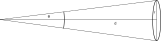
\includegraphics[width=0.8\columnwidth]{SmallAngles.pdf}
\includegraphics[width=0.4\columnwidth]{Eprofile_Lightson_Example.jpg}\includegraphics[width=0.4\columnwidth]{Eprofile_Grid_Example.jpg}
\caption{Eprofile example with grid. Left: reference, right: eprofile signal with grid.}
\end{figure}

Assume a point source that propagates and diverges over a distance $d$ until it is detected at the beam profile, now extending to a circle of radius $r$. If $d \gg r$, then the small angle approximation holds:

\begin{equation}
\tan \theta \approx \sin \theta \approx \theta, \quad \sin \theta = \frac{r}{d} \longrightarrow \theta \approx \frac{r}{d},
\end{equation}
where $\theta$ denotes the divergence, equivalent to the ratio of forwards to transverse momentum, $p_\parallel/p_\perp$.
\vspace{\baselineskip}

The pointing fluctuations of the beam can be estimated similarly if one suspects mainly an angular jitter. In reality the pointing will be related to a combination of translation and rotation, where a transverse displacement of the beam is typically of order $\sim \mu m$ and will then over the course of a drift be dominated by the angular displacement.

To obtain an absolute number for the divergence and pointing the screen has to be spatially calibrated. This includes characterising the relative angle of screen, camera and laser axis.
A regular grid of known dimensions, for instance printed on some paper, can be used as spatial reference to evaluate the relative angle of camera and screen. The angle of the screen relative to the beam has to be measured separately. 
One way to compensate both is to place the screen at 45 degrees to the beam and the camera looking at 45 degrees as well restoring the right dimensions.

\subsection{Magnetic Energy Spectrometer}

The energy of electrons in wakefield experiments can be determined in experiment using a spectrometer based on magnetic dispersion. The electrons are deflected using a dipole magnet and are detected on a scintillating Lanex screen.

In order to understand the fundamental relations this method is based on, the motion of a single electron in a homogeneous magnetic field is considered and analytically solved in the case of an electron passing through a region of a homogeneous magnetic field of finite extent, but without considering fringe fields or gradients. In reality, the magnetic fields are measured or simulated and particle tracked using numerical methods.
\vspace{\baselineskip}

Consider an external magnetic field restricted to a circle of radius $r_b$ embedded in an otherwise completely field-free region. The following derivation is based on Stuart Mangles' (Imperial College) PhD thesis \cite{ManglesThesis}.
\begin{align}
\mathbf{B} &= B \mathbf{e_z} \, &r \leq r_b,\nonumber \\
&= \mathbf{0} &r > r_b
\end{align}

The angular deflection of a particle in this case can be solved analytically using the Larmor radius and simple geometry.

\begin{figure}
\centering
\includegraphics[height=0.3\columnwidth]{elecspec.png}\includegraphics[height=0.3\columnwidth]{Espec_shotexemp.jpg}
\includegraphics[width=0.75\columnwidth]{TrackingFigMangles2015.png}
\caption[Visualisation of an electron deflected in a homogeneous magnetic field and ]{Visualisation of an electron deflected in a homogeneous circular magnetic field (grey) with radius $r_b$. The larger green circle indicates the Larmor radius, determining the electron trajectory (blue) from the point of entry into the field (A) to its exit point (C) resulting in a total deflection $\theta$. Bottom: Example of particle tracking through a three-piece magnet for electrons of -X, 0 and +X MRAD pointing.}
\end{figure}

Drawing the circular field region for the magnetic field and the electron entering the field, one can then graphically indicate its Larmor radius, equivalent to its expected motion for the region with the constant B-field. The angles in this constellation are determined using the trigonometric relation that the angles in a triangle have to add up to $\pi$:
\begin{equation}
2 \alpha + \theta = \pi,
\end{equation}
where $\theta$ is the deflection angle and $\alpha$ the angle indicated in the graphic (see figure).

Relating this to the angles to substitute $\alpha$:
\begin{equation}
\tan \alpha = \frac{r_L}{r_b},
\end{equation}
and then expressing this into parameters we can measure in experiment we reach
\begin{align}
\tan \frac{\theta}{2} &= \frac{r_b}{r_L},\nonumber\\
&= \frac{e B r_b}{p_\perp}.
\end{align}

In a typical LWFA experiment $p_\perp$ will be dominated by the component in the laser propagation axis, i.e. if the propagation axis were z, $|\mathbf{p_\perp}| \approx p_z$. 
\vspace{\baselineskip}

\iffalse
\begin{figure}[h]
\centering
\includegraphics[width=0.75\columnwidth]{ExpSetup_GasJet_MagnetOnly.pdf}
\caption{Sketch of a typical spectrometer setup in a LWFA experiment (left). The relativistic electron (blue) beam enters the dipole magnet (grey) and is dispersed onto the lanex screen according to its energy. Higher energies are deflected less than lower energies. The image on the right is an example of a spectrum taken on an experiment. The high energies are on the bottom of the spectrum decrease with height upwards.}
\end{figure}
\fi

The correct assignment of the position on the screen to the correct electron energy is achieved by measuring the position of all components (lanex screen, magnet, TCC) and mapping the magnet field strength accurately, for instance using a Hall probe, and then running a particle tracking code with these details.
Each pixel has a certain error bar on its associated energy as the divergence of the electron beam (instrument function), an offset at source or shot-to-shot pointing fluctuations could lead to different positions at the same electron energy (pointing). The energy resolution is determined by the strength of the magnetic field, the drift length, the intrinsic spatial resolution of the scintillator (for Lanex $\sim 100\,\mathrm{\mu m}$ REF) and the spatial resolution of the imaging system. 
\vspace{\baselineskip}

A second Lanex screen or other spatial references (fiudicials) can help to identify and correct for pointing fluctuations or an overall pointing to achieve a more accurate determination of the energy, but could introduce additional scattering. See Kristjan Poder's PhD thesis \cite{PoderThesis} for more details on this or for instance \cite{Soloviev2011_TWOSCREEN}.

The width of the electron trace in the non-dispersion direction can be used to determine the divergence of the beam (in the non-dispersion axis) and cross-checked with the spectrum of the betatron radiation or a beam profile monitor.
\vspace{\baselineskip}

In addition to measuring the distances and the magnetic field, the imaging system for the scintillator screen has to be characterised.
This requires transforming the optical image (projective transform), spatially calibrate the image and translate from spatial to energy axis.
More details on the typical procedure can be found, for instance, in Jason Cole's or Kristjan Poder's PhD thesis \cite{ColeThesis, PoderThesis}

In all Chapters Lanex (standard and Biomax) are used in conjunction with Andor Neo cameras.

\iffalse
%\subsubsection{Multiple screens and deconvolution}

In a magnetic spectrometer electrons are being dispersed in one axis and the spectrum can be deduced from the fan of electrons and the position at a detector screen. Whereas the spatial extent in the non-dispersion direction tells us the divergence of the beam in that axis as it is approximately unperturbed, the divergence of the beam in the dispersion direction is convolved with the magnetic dispersion. At the same time an overall pointing of the beam could lead to an overestimate or underestimate of the actual energy. In order to be able to correct for these factors several points of reference are required. The source position has to be known along with two more measurements. This could be two screens or a spatial feature (fiudicial) and one screen.
A simple symmetry assumption mainly allows adding an error bar to the maximum energy within a reasonable limit.

Two screen tracking: forwards or backwards method.
Run tracking with a variety of angles for identical energies. Check what energy estimate each screen gives at a distinct feature. See if there are any deviations, try the next angle and find the least square fit.
The other approach is backtracking but this is more complicated.

If one has a fiudicial no explicit features in the beam are required as the fiudicial will become that feature. However, the positions have to be measured to a high precision to be able to distinguish sensible pointing shifts.

Either methods can be used to deconvolve the spectrum and iteratively find the real energy spectrum underlying the measured distribution. More screens can increase the accuracy but the scattering of the beam passing through lanex becomes quite evident and distinct features blur out when drifting further because of this.
\fi

\subsection{Absolute Charge Measurement}

Absolute charge measurements are challenging in an EMP rich environment as near intense laser-plasma interactions.

Commonly, Lanex or other scintillators imaged by optical CCD cameras are used to measure the electron spectrum and charge.
However, obtaining an absolute charge calibration requires a very detailed knowledge of the efficiencies of the scintillator material, imaging system, quantum efficiency of the detector chip and so on (REF REF). Typically, phosphorescent image plates (WHAT ARE THEY MADE OF) are used instead to achieve an absolute calibration (REF).

In the experiments described image plate was attached to the back of the electron spectrometer screen and left in the beam path for several shots. After removing the image plate again they are left to decay over a certain period before then being analysed using a scanner. The accumulated signature on the image plates was then overlapped with the corresponding scintillator images taken with the optical cameras to obtain a conversion factor of pixel counts to charge. The scattering and damping of the imaging plate has to be considered and its heightened sensitivity which might result in additional background noise on the imaging plate due to its large dynamic range.

The disadvantage of imaging plate technology is that it is not suitable for high repetition rate operation as it has to be replaced manually. In addition, any change of the imaging system requires a new calibration which could be intrusive and time-constraining depending on the spectrometer setup (vacuum or air?).
The evaluation of the diagnostic is also not instantaneous as it has to be left to decay and then scanned.
\vspace{\baselineskip}

Other technology being used are ICT, but they have to be shielded properly as electronics is vulnerable in EMP environment and are very expensive.


ADD A REFERENCE THAT DESCRIBES THE PROCEDURE IN MORE DETAIL, ON ABSOLUTE CALIBRATION.



\section{X-ray and Gamma-ray Diagnostics}

Wakefield acceleration has not only demonstrated to be a feasible tool to accelerate electrons to a GeV scale, but has also been shown to be a useful source of X-rays of remarkable brightness by the means of betatron radiation \cite{Rousse2004_BETATRON,Kneip2010_BETATRON}, as a tunable all-optical Compton-source \cite{TaPhuoc2012_ICS} and as bremsstrahlung source \cite{Glinec2005_Brems,Cipiccia2012_Brems}. In addition, using LWFA electron beams for FEL operations has become an active field of research itself (REF REF).

The following section addresses different diagnostics to characterise high-energy radiation produced using an LWFA source, laser-solid, laser-electron and electron-solid interactions.

\subsubsection{Motivation for variety of diagnostics}

In the following chapters various arrays of scintillator arrays (in this case caesium-iodide doped with thallium, CsI(Tl)) are employed to measure the spectrum of gamma radiation from various sources (bremsstrahlung, linear and non-linear inverse Compton scattering and hard betatron radiation).


In the soft and hard X-ray regime spectra can be deduced by comparing the transmission of the radiation through various materials with characteristic K-absorption edges (REF), Ross filter pairs (REF) or relying on crystal reflections matching the Bragg-condition (REF) or a combination of both.
For these conditions a good knowledge of the material properties and the positioning of the crystal and cameras is essential.
The energy-dependent transmission through the material is related to an interplay of different mechanisms (Compton scattering, Rayleigh scattering, photoelectric effect, pair production and so on). The sum of these cross sections can be combined and found in specific repositories (REF NIST).

At higher X-ray energies entering the gamma regime $\hbar \omega \rightarrow 1\,\mathrm{MeV}$ K-edges to effectively distinguish spectral bands become rarer and most materials become more transparent, as a consequence resolving a full spectrum becomes challenging. At the same time incoherent scattering becomes more dominant and pair production becomes possible, with increasing likelihood at higher energies (see cross section PLOT XX REF).
\begin{figure}
\centering
\includegraphics[width=0.5\columnwidth]{XsecCsI.png}\includegraphics[width=0.5\columnwidth]{XsecLi.png}
\caption{Mass attenuation of CsI (left) and Li (right).}
\end{figure}

At the few MeV level the spectrum of the generated electron-positron pairs scales directly with the energy of the gamma radiation interacting with the matter through Compton scattering (incoherent scattering) and pair production (REF). Measuring the spectrum of these particles, for instance with a magnetic spectrometer setup, and comparing the results with a simulation result can then be used to deduce a gamma spectrum \cite{Corvan2014_Gamma}. This works particularly well for low-Z materials as lithium (see PLOT) where the cross section for incoherent scattering dominates but also varies whilst the pair production cross section also strongly varies giving the diagnostic additional sensitivity.

\EliasComm{I checked and kevlar (so kapton will be very similar) has similar cross section for processes in the MeV range, so the vacuum window could act as converter.}

The spectrum of the pairs, however, becomes less sensitive to the energy of the gamma-radiation at higher (tens of MeV) energies (XSEC XX PIC REF). An alternative method to measure such a hard spectrum is tracking the energy deposition of radiation and secondary sources throughout an array of scintillator material until it decays, effectively measuring the length and shape of the cascade.
This method has the advantage of being variable and viable for the few MeV level and much harder radiation.

Simulations linked to this technique are outlined in this work and are then applied to experimental data in the following chapters to measure radiation from different materials in a range of hundreds of keV to hundred MeV (over three orders of magnitude).

A detector interacting with such high energetic gamma-radiation is now faced with energy deposition by the radiation itself and secondary particles and radiation. An extended detector can mitigate this effect by forcing pair production in an earlier part of the detector and performing an again well resolved measurement in a second part of the detector. The complex interplay of pair production and energy deposition from secondary sources requires numerical solutions calculating the cross-sections for various processes dynamically throughout the interaction with the detector. The extended detector acts as an imperfect calorimeter with some energy resolution. This is where GEANT4 \cite{GEANT4} or other Monte Carlo based simulation codes come into play (e.g. \cite{MCNP}).

\subsection{Pinhole Camera}

A pinhole camera is a relatively simple diagnostic that allows measuring the source size and estimate the flux of an X-ray source.

CCD Chip, pinhole of right material on tube to shield noise, source. Relative distances determine the magnification (geometric magnification).

geometric magnification M: distance camera to source
\begin{equation}
M = \frac{d_{cam-pin}}{d_{source-pin}}
\end{equation}


Used on the experiment described in Chapter XX.

Double pinhole, one with 5 um aluminium and one with 6 um PET filtering. The pinhole itself is made of 25 um Ta.
X-ray cameras used are DX420-BR-DD Andor in-vacuum cameras with XX times XX chips each XX times XX microns. These are sensitive to X-rays, see QE curves XX REF. Quite often with beryllium window or filtering in front of the chip.

Alignment can be done by adding a spike on the front, point it at the interaction point and then carefully removing it at the end.

By comparing the transmission of the two spots (using a double pinhole) gives an estimate how much energy is in one band and another, especially if the K-edges are chosen correctly.
\begin{figure}
\centering
\includegraphics[width=0.9\columnwidth]{PinholeCamera.png}
\includegraphics[width=0.9\columnwidth]{20180326r001s002_PinholeCam.jpg}
\caption[Example of pinhole camera image.]{Top: Sketch of a pinhole camera. Bottom: Example of a double pinhole camera image taken on a recent experimental campaign. The pinholes were filtered differently, such that the pinholes measure the flux in different spectral intervals.}
\end{figure}

\EliasComm{Refer to BK's thesis \cite{KettleThesis}.}


\subsection{Crystal Spectrometer}

Bragg condition and crystal, CCD camera.
Applicable in any range accessible using lattice constants. Energy range depends on detector size, distance and lattice properties.

Bent crystals can be used for focusing and larger spectral range.
HAPG HOPG with mosaicity to increase reflectivity.

Bragg's law

\begin{equation}
n \lambda = 2 d \sin \theta
\end{equation}

Energy spread/error on the camera based on initial divergence.

Efficiency needs to include reflectivity of crystal, filtering, quantum efficiency and so on. Thermal noise.

Used in experiment described in Chapter \ref{Chap:BW}.
\begin{figure}
\centering
\includegraphics[width=0.5\columnwidth]{CrystalSpecCamera.png}
\includegraphics[width=0.9\columnwidth]{CrystalSpec.pdf}
\caption[Sketch of a crystal spectrometer setup.]{Top: Sketch of a crystal spectrometer setup. X-rays are dispersed onto a CCD chip. Bottom: Example of a spectrum measured in a crystal spectrometer setup. The X-rays are dispersed spectrally in the x-axis with distinct emission lines. The central part is filtered with aluminium, resulting in a sharp cut-off due to the K-edge, which can be used as calibration.}
\end{figure}

\EliasComm{Refer to BK's thesis \cite{KettleThesis}}

Andor DX420 in-vacuum cameras (since we are looking at very fine resolution and low energies).

Pixel size for the cameras and typical filtering.

REF BK thesis, sketch also based on one of his sketches.

Applications for XANES measurements due to good resolution \cite{Kettle2019_XANES}.

The K-edge of a filter can be used to get an on-shot energy reference to calibrate the image. Two different materials would make this even clearer.
The sharpness of the edge could be an indicator of energy spread/divergence impact. Few eV resolution.

See FIGURE REF for example of a spectrum taken on an experiment. Spectral lines and K-edge from aluminium filter.

In this range the accurate knowledge of the filtering (micron thickness) is crucial as this is the few keV range.

Have to use in-vacuum as going through a window would result in cut-out of the relevant signal.

\subsection{Filter Packs}

Typically used for X-ray measurements on LWFA experiments (betatron radiation) are filter packs or arrays of materials of varying K-edge over the range of X-ray energies expected. By comparison of the transmission through the materials and assuming a spectral shape, the spectrum can be estimated. The profile of the radiation is also measured but has to be corrected for when comparing the transmissions.

Direct (CCD) or indirect detection (with scintillator) Andor iKon.


\begin{figure}[h]
\centering
\includegraphics[width=0.9\columnwidth]{filter_pack_sketch.pdf}
\caption{Sketch of a typical betatron setup.}
\end{figure}


\begin{figure}
\centering
\includegraphics[width=0.3\columnwidth]{FilterPack.png}\includegraphics[width=0.3\columnwidth]{FilterPackX.png}
%\includegraphics[width=0.3\columnwidth]{QE_BR_DD.png}\includegraphics[width=0.3\columnwidth]{DeltaEcrit.png}
\caption{Images of filter packs.}
\end{figure}

When X-rays increase in energy the quantum efficiency of the CCD chip decreases, so energies beyond 100 keV are not measured.

More details on the extraction procedure can be found in Jonathan Wood's PhD thesis \cite{WoodThesis}.

Was not used on the experiments described in this work but other relevant experiments.
To motivate why other indirect detection methods are required and this method becomes less sensitive at higher energies.

If we assume only absorption following Beer's law, the signal through a filter on the camera including quantum efficiencies (QE) etc. (taken from Jonathan Wood's PhD thesis \cite{WoodThesis})

\begin{equation}
Y_i = A \int^{E_{max}}_{E_{min}} E \,S(E) \,Q(E) \,T_i(E) \,\mathrm{d}E
\end{equation}

Then minimise (least square) the transmissions for a spectrum S(E).

\subsection{Gamma-ray Scintillator Profile}

Once the energies reach the gamma-ray regime (> 1 MeV), even using an indirect-detection camera on axis becomes infeasible as photons will decay into secondary particles and radiation that will shower the camera and reduce its lifetime.

Relying on indirect detection with an off-axis camera or detector then becomes necessary. 
In experiment this has been an array of scintillator material normal to the beam axis and imaged by a camera.

This enables measuring the shape of the profile is interesting as it allows deduction of the source (SEE REF). In this context it gives insight into the properties of the electrons (their divergence, propagation and so on). 
The profile is also an indicator the the intensity of the interaction in non-linear ICS and carries the imprint of the interacting electron beam within it.
It is hence a useful diagnostic to not only confirm an interaction took place but also to characterise the conditions at the interaction.

\EliasComm{Reference REF UMSTADTER AO? TOM BLACKBURN IF PUBLISHED.}

\subsubsection{Experimental Implementation}

In these experiments caesium-iodide doped with thallium is used frequently due to its high light yield. LANEX has typically a better spatial resolution due to its fine grain size ($\sim 100\,\mathrm{\mu m}$) but the energy deposition in the thin screens, especially at gamma-ray energies, is not sufficient to produce a lot of signal. Long CsI crystals give a pixelated response. LYSO also comes at a decent resolution but the light yield is lower. It is a fast scintillator but at lower repetition rates as at Gemini, this is not necessary and the noise levels can not be gated away as it is too close.

\begin{figure}
\centering
\includegraphics[height=0.3\columnwidth]{JenaProfile.jpg}\includegraphics[height=.3\columnwidth]{ScreenshotGEANT_JenaStack.png}\includegraphics[height=0.3\columnwidth]{20190208r015s036_GammaProfile_crop.jpg}
\caption[Scintillator profile screen, photograph, GEANT representation and measured gamma signal.]{Example of a scintillator stack used as profile screen in experiment. Photograph of the scintillator screen (left) along its GEANT representation (middle) and gamma signal measured with the stack in experiment (right).}
\end{figure}

Different profile screens were used in the experiments. The details can be found in Table XX NUMBER REF.

The scintillators emit around 546 nm (XX NUMBER) of radiation which is ideal for CCD chips. Andor iXon cameras (sensitive chips) are used to image the scintillators close to normal or using a mirror. A bandpass filter can be used to reduce the noise.


\begin{table}[h]
\centering
\begin{tabular}{l|l|l|l|r|r}
Name & Chapter &Crystals & Crystal Dimension & Front Plate & Divider\\ \hline \hline
QUB & \ref{Chap:BW}, BW & $20 \times 20$ & $2 \times 2 \times 20$ mm & Al 10 mm & Al 0.1 mm\\
Jena & \ref{Chap:linICS}, linICS & $45 \times 45$ & $1 \times 1 \times 10$ mm & TiO2 0.5 mm & TiO2 0.2 mm\\
DESY & \ref{Chap:linICS}, linICS & $30 \times 30$ & $1.5 \times 1.5 \times 10$ mm & Epoxy 0.5 mm & Epoxy 0.2 mm\\
RAL & \ref{Chap:RR15}, RR & $47 \times 33$ & $5 \times 5 \times 50$ mm & None & Al 1 mm
\end{tabular}
\caption[Overview of CsI profile screens used in experiments.]{Overview of caesium-iodide crystal stacks used in experiments as profile screens.}
\end{table}

The photons go through the entire thickness of 10 mm CsI, so background subtraction from random noise was not a large concern. The signal is strong, also due to the high light yield of CsI at cost of spatial resolution (1mm crystals). The crystal outlines themselves and the overall array act as spatial reference as their symmetry is well known. A close to normal orientation is preferable to discourage mixing and again a normal imaging is ideal as well, resulting in very little post-processing being required.



\subsubsection{GEANT simulations showing energy deposition}

\EliasComm{Add a figure on energy deposition using GEANT REF for MeV range and on the other hand absorption using Henke.}
RESULT: The energy deposited in an energy range (GIVE GEANT SIM FOR 10-XX MEV) is proportional to the energy of the radiation.

\EliasComm{Add comment on GEANT code in general, REF GEANT, mention Jason's and Kris' input.}

When planning to use such a detector as measurement of the total energy of the radiation one has to keep in mind that this is not a calorimeter in the gamma regime as radiation is bound to be transmitted through the stack. However, it is expected that the energy deposited per photon will vary and of course the number of photons will leave their trace on this detector.

The response is simulated using GEANT:
The detector in the simulation:
the detector assembled in the simulation is based on a CsI stack used in some experiments and provided by the Helmholtz Institut in Jena.
It consists of 45 x 45 CsI(Tl) crystals of face dimension 1 mm x 1 mm and a thickness of 10 mm. The crystals are spaced by a 0.2 mm layer of TiO2 and the front side has another layer of TiO2 of 0.5 mm which holds the entire stack together.

The stack was defined as such in the simulation and it can be seen in Figure ADD HERE.


The front side of the detector is XX m away from the source of the radiation, similarly to experiment conditions, hence being in general able to cover plus minus NUMBER divergence from a point source if centred along the same axis.

Now individual photons with ranging energy from 10 keV to 500 MeV are launched from the source point and the energy deposited in the crystals is being recorded. Each energy step is simulated 10.000 to 100.000 times and then averaged to obtain an average energy deposited per photon of this energy.

The results from these simulation can be seen in figure ADD HERE. Photon energies up to ENERGY are almost completely absorbed, backscattered and rarely transmitted. At around 200 keV suddenly a large amount of radiation is being absorbed. This indicates a material characteristic absorption edge.
This means that whilst for the majority of the energy ranges the CsI profile will give a good indication as energy times flux is monotonic increasing and somewhat linear for the two regimes of interest. In the regime of hundreds of keV we have to consider that a lot of energy will be absorbed in the front layer and we have to check how this behaves further downstream in the next detector.

\begin{figure}
\centering
\includegraphics[width=.5\columnwidth]{Edep_JenaStack.pdf}\includegraphics[width=.5\columnwidth]{Edep_JenaStack_rel.pdf}
\caption{Simulation results: energy deposited per photon in a profile stack. Replace this by 10's MeV plot as GEANT is not performing too well at low keV levels and the 250 keV peak might be a fluke.}
\end{figure}

If we look at this in terms of relative energy deposited per photon, so in other words energy deposited over energy of the photon, this does not look like a sharp edge but merely a steady decrease in energy deposited relative to the total photon energy. Scattering cross sections typically decrease with increase in energy and this goes along the same lines.


\subsubsection{Absolute Calibration}

The smaller profile stacks can also be calibrated by using a radioactive source since the stack mainly consists of crystals.
A Na or Cs source can be used at the standard measurement conditions. The energy emission is well known. If one assumes that all energy is absorbed by the detector the light yield is related to energy deposited. The disadvantage to real calorimeters is that due to a non-zero transmission through the material and due to the spacers not all energy deposited is deposited within crystals and converted into signal.



\subsection{Gamma-ray Converter Spectrometer}

At gamma-ray energies above $2m_e c^2 \approx 1\,\mathrm{MeV}$ one photon can generate a pair of electron-positron pairs when scattering from matter using the electric field of the nucleus or the valence electrons as interaction partners. The maximum energy of the generated electrons and positrons are determined by the energy of the gamma photon, the overall spectrum is close to exponential (SEE THEORY INSERT REF, BETHE HEITLER). Based on this principle one method to measure the gamma spectrum is using a sheet of high-Z material to convert the gamma rays into matter and then measure the spectrum of these particles in a magnetic spectrometer (REF).
\EliasComm{Need to rework this part since it is not just pair production but also Compton scattering.}
In the range of few to maybe 30 MeV the cross section rises rapidly (SEE FIGURE XX NUMBER) compensating for the fewer pairs at higher energies and making this a feasible spectrometer to resolve the full spectrum in this range \cite{Corvan2014_Gamma}. At higher energies the cross-section flattens which means that the contribution to the total production of pair equalises over all energies but due to the exponential spectrum of the pairs produced very few pairs at the maximum photon energies are produced.
The Compton spectrometer becomes a pair spectrometer and the signal-to-noise ratio and sensitivities become more important, meaning more space is required to resolve those energies since the higher energy pairs now require stronger magnets, more drift and need to clear away from the noisy axis.
 
\begin{figure}
\centering
\includegraphics[width=0.5\columnwidth]{CorvanSpectrometer.png}
\caption[Sketch of a Compton spectrometer design.]{Sketch of a Compton spectrometer design: gamma rays enter the setup from the left side and enter a block of lithium, releasing electrons through Compton scattering and depending on the energy also electron-positron pairs. A magnetic field disperses electron and positrons onto detector screens. Reprinted from \cite{Corvan2014_Gamma}, with the permission of AIP Publishing.}
\end{figure}



\chapter{First Measurements of Radiation Reaction at Astra Gemini}
\label{Chap:RR15}

\section{Experimental Motivation}

\subsubsection{Inverse Compton Scattering}
In relativistic inverse Compton scattering (ICS) one (linear) or multiple (non-linear) photons scatter from a relativistic electron ($\epsilon/m_e c^2 = \gamma \gg 1$). The scattered photons experience a relativistic Doppler-shift and are re-emitted in a narrow cone of divergence $\sim 1/\gamma$ in the direction of the electron propagation, carrying a higher energy based on the electron energy and the intensity of the laser field. The emitted photon energy, $E_{ph}'$, is maximised in a head-on collision: $E_{ph}' = 2 \gamma^2 (1-\cos\theta)E_{ph}$ (see e.g. \cite{Esarey1993_NT,Lau2003_NT} or also the \nameref{Chap:Theory} Chapter of this thesis). Higher electron energies result in a stronger shift of the radiation, leading to a hardening of the spectrum and an increase of the corresponding energy loss the electrons experience. A more intense laser field ($a_0 > 1$), on the other hand, enables non-linear interactions and increases the number of photons interacting at once with an electron, resulting in the generation of $\sim a^3_0$ higher harmonics  but also redshifting and broadening of the spectrum. As a result the rapidly increasing number of higher harmonics blend together to form a broadband synchrotron-like spectrum.

ICS provides a promising route to generate bright burst of high energy radiation reaching 100's of keV or even MeV photon energy, suitable for medical and imaging applications (also of high-Z objects) and to stimulate nuclear transitions, even at small-scale facilities \cite{Albert2016_APP}.
It also provides a useful tool to measure beam properties \cite{Kramer2018_Gamma}, including polarisation \cite{Baylac2002_POL,Barber1993_POL}.
In addition, the high photon energies offer the opportunity to directly observe the energy loss, if the emitted photon carries an energy comparable to the energy of the electron, and to measure the effect of radiation reaction on the beam dynamics itself when the electric field in the rest frame of the electron approaches the critical field of QED, $E_{crit}$. Classical descriptions of radiation reaction exhibit unphysical predictions like self-acceleration, resulting in runaway solutions, or an unbounded emission spectrum, i.e. energy loss higher than the initial energy of the electron is allowed. A universally accepted description of radiation reaction has not been found yet.

\subsubsection{Inverse Compton Scattering using Laser Wakefield Accelerators}

In LWFA the intense laser driver is intrinsically synchronised to the relativistic electron beam that trails behind it, which makes LWFA well suited to study inverse Compton scattering at high intensities.
\vspace{\baselineskip}

\begin{figure}[h]
\centering
\includegraphics[width=0.8\columnwidth]{RR2015_Gmax_thiswork.pdf}
\includegraphics[width=0.8\columnwidth]{RR2015_Eta_thiswork_lowera0.pdf}
\caption{Comparison of all-optical ICS experiments using LWFA. The circles (cyan) indicate one-beam experiments that use a plasma mirror to reflect the LWFA driver beam and scatter off the electron bunch it accelerated before. The triangles (blue and green) indicate experiments that used two laser beams, one to accelerate electrons from LWFA and one separate laser to scatter off them. Top: Maximum gamma energies measured and their year of publication. Bottom: Electron energies and laser intensities in recent ICS experiments using LWFA. The contour lines indicate the corresponding values of the quantum nonlinearity parameter $\eta$.}
\end{figure}

Colliding-pulse or ICS experiments using LWFA have been successfully performed by different groups over the past years, gradually improving the control over the process, increasing the laser intensities and the energies of the electrons involved, and subsequently of the radiation generated \cite{TaPhuoc2012_ICS,Chen2013_ICS,Liu2014_ICS,Powers2014_ICS,Sarri2014_ICS,Khrennikov2015_ICS, Yan2017_ICS, Shaw2017_ICS}. 
The energy and the tunability of the produced radiation is a good indicator for the continuing progress of these experiments. More specifically of interest for measuring radiation reaction is the quantum non-linearity parameter, $\eta = 2\gamma E_L/E_{crit}$ \cite{Ritus1985_QRR,Bell2008_PairsEta}, that indicates the strength of the electric field of the laser in the rest frame of the electron relative to the critical electric field of QED, $E_{crit}$, also called the Schwinger field.

\subsubsection{Inverse Compton Scattering using a plasma mirror}

A single intense laser pulse can be used to accelerate electrons to relativistic energies via LWFA and to scatter the electrons after backreflecting the laser from a close-to-normal plasma mirror \cite{Kapteyn1991_PM} (e.g. tape \cite{TaPhuoc2012_ICS}). In this geometry the laser beam and the electrons are timed intrinsically. In \cite{TaPhuoc2012_ICS} electrons of an energy $\sim 100\,\mathrm{MeV}$ were collided at a laser intensity of $a_0 \approx 1.2$ (weakly non-linear). The radiation measured was a broadband X-ray spectrum and reached up to $100'\mathrm{s}\,\mathrm{keV}$ photon energies. A lower electron energy spread and tunability was demonstrated at slightly lower electron energies and laser intensities in \cite{Powers2014_ICS} and\cite{Khrennikov2015_ICS}. In \cite{Tsai2015_ICS} a low energy spread electron beam of up to $90\,\mathrm{MeV}$ was scattered at a laser intensity $a_0 \approx 1.2$, producing an X-ray spectrum peaked at $180\,\mathrm{keV}$. 
By now the highest recorded gamma-ray energies from ICS in LWFA using this scheme have reported in \cite{Shaw2017_ICS} reaching up to $85 \,\mathrm{MeV}$ photon energies in a collision with electrons at energies up to $2\,\mathrm{GeV}$.
\vspace{\baselineskip}

Whilst this technique avoids issues with timing and overlap, the intensity of the laser pulse is limited as it is partly depleted when interacting with the electron bunch after driving a wake and is typically not tightly focused. At the same time the acceleration can not be pushed to its depletion limit as the laser pulse has to remain intense enough for a suitable interaction. Further problems might arise as controlling or measuring the wavefront of the depleted laser pulse is challenging. The electrons will also produce radiation from bremsstrahlung when passing through the plasma mirror, which overlays the ICS signal, although in \cite{Tsai2015_ICS} the measured signal was claimed to be insignificant.
These details are important for a precise measurement of radiation reaction, but might be of secondary concern if a well-defined spectrum is not crucial for the application.
At facilities housing the next generation of PW lasers, the reflective scheme will also be able to yield very promising results to probe radiation reaction.

\subsubsection{Inverse Compton Scattering with two lasers}

If two separate lasers are available or maybe one very powerful laser can be split into two parts, one can be used to accelerate electrons via LWFA and one to scatter off them. Electrons produced from LWFA are typically very short in duration $\sim 10's \,\mathrm{fs}$ \cite{Lundh2011_BUNCH} and only few microns small \cite{Weingartner2012_BUNCH} when leaving the accelerating cavity. This allows focusing the second laser very tightly to reach high intensities and to interact with a large fraction of the electron bunch at comparable intensities without a large background from linear ICS. Using two laser pulses opens the gateway to combine higher intensities and electron energies at the interaction point, and gives more control over the interaction itself. However, it is challenging to overlap the micron-sized electron bunch with the ultra-short tightly-focused laser pulse, compressed in time and space, and to maintain this alignment over an extended period of time \cite{Samarin2017_RR}.

A very powerful laser can also be used to interact at slightly larger spot sizes, which improves the probability of interactions as it mitigates relative pointing fluctuations. If the laser spot is larger than the electron beam the theoretical modelling of the interaction can be simplified as all electrons approximately experience the same field (REF) and focusing effects are negligible \cite{Harvey2016_ICSFOCUS}.

In \cite{Chen2013_ICS} relativistic electrons were scattered at an angle of $10$ degrees and $1\,\mathrm{MeV}$ gamma rays were produced. In \cite{Liu2014_ICS} an electron beam of $\epsilon = 450\,\mathrm{MeV}$ was scattered with a second harmonic laser at $E_{ph} = 3\,\mathrm{eV}$  reaching up to $9\,\mathrm{MeV}$ gamma energies.
In \cite{Sarri2014_ICS} electrons at an energy of $400 \, \mathrm{MeV}$ were successfully collided at an laser intensity of $a_0 \approx 2$, resulting in broadband radiation extending up to $18\,\mathrm{MeV}$. In \cite{Yan2017_ICS} electrons of energy $\sim 200\,\mathrm{MeV}$ were collided with an intense laser at $a_0 \sim 12$ reaching photon energies just above $20\,\mathrm{MeV}$, resulting in the generation of over $500$ orders of higher harmonics.

\subsubsection{Future LWFA Studies on Inverse Compton Scattering and Radiation Reaction}

Future laser facilities will be able to perform ICS studies at even higher electron energies and laser intensities.
Several PW laser systems have already or are soon to commence their operation, with some existing laser systems being upgraded to the PW-level as well (for instance ELI-NP \cite{Gales2018_ELINP}, ELI-Beamlines \cite{Weber2017_ELIBeamlines}, EPAC (no REF), HERCULES \cite{Yanovsky2008_HERCULES}, Apollon \cite{Zou2015_Apollon}, SULF \cite{Li2017_SULF}, BELLA, XCELS, CALA). At this point, QED studies are already considered for the 100 PW regime \cite{Shen2018_SULF}. 
Maximum electron energies from LWFA on the other hand have reached the multi-GeV regime \cite{Kim2013_GEV,Leemans2014_GEV} with up to 8 GeV recently \cite{Gonsalves2019_GEV}.

The combination of both, highly relativistic electron beams and highly intense lasers, opens up a wide variety of research topics in the strongly non-linear quantum regime probing radiation reaction\cite{Blackburn2014_QRR}, photon-photon scattering \cite{Enterria2013_PhPh} and pair production from the Breit-Wheeler mechanism \cite{Pike2014_BW,Blackburn2017_pairs} or by reaching supercritical field strenghts \cite{Blackburn2019_SUPER}. The high laser intensities will also enable studies of vacuum birefringence \cite{King2016_VB}.

Considering the cost and variety of facilities, it is important to investigate the limitations of current all-optical ICS setups, the feasibility of future measurements and explore potential ways to improve them \cite{Samarin2017_RR}.

\subsubsection{Inverse Compton Scattering at conventional accelerator facilities}

Inverse Compton Scattering has been employed at conventional accelerator facilities for some time as well, but at much lower laser intensities to measure the beam polarisation (polarimetry, e.g. \cite{Baylac2002_POL,Barber1993_POL}), in particular in the context of (de)polarisation of beams due to the Sokolov-Ternov effect\cite{SokolovTernov1964_POL,Baier1967_POL}, or as beam diagnostics \cite{Bosco2008_LW}.

As the field of applications for large-scale accelerators widens and the access to 10 TW laser systems and even commercially available PW-class lasers becomes easier, conventional accelerators combine their high-quality relativistic particle beams with intense laser pulses.
At XFELs, for instance, this is interesting for the study of warm-dense-matter states (REF) and high-energy-density physics (HEDP) (REF), involving pump-probe measurements, where X-rays from an insertion device probe matter structures and changes induced in them in interaction with a laser (REF).
In the wake of increasing interest in measuring QED phenomena in laser interactions, ICS has also moved into the focus of conventional accelerator facilities. New dedicated projects like LUXE at the X-FEL Hamburg \cite{Burkart2019_LUXE} and the SFQED project at FACET-II (30 TW, 13 GeV XX NUMBERS?) aim to continue where the seminal E144 experiment at SLAC left off in the 90s, where a 46 GeV electron beam was collided with a laser of intensity $a_0 \sim 0.3$ \cite{Bula1996_RR,Burke1997_RR}. Whilst the high-quality beams at these facilities are superior to LWFA studies in terms of charge, energy and energy stability, these projects are facing other challenges due to significant amount of background noise in the accelerator tunnels, and typically longer and larger electron bunch sizes resulting in a significant overlay from linear scattering events in an ICS setup.

Another measurement of radiation reaction was performed at the LHC \cite{Wistisen2018_RR}, however using positrons and planar channeling in crystals instead of ICS as tool.

An overview over the high field QED projects currently being undertaken can be found in \cite{SFQEDOverview2019}.

\section{Chapter Outline}

The work presented in this chapter relates to an ICS experiment aimed at measuring radiation reaction performed at the Gemini laser facility in late 2015. The experimental team succeeded in colliding electrons of energy $\epsilon \approx 550\,\mathrm{MeV}$ at a laser intensity of $a_0 \approx 10$, reaching critical gamma-ray energies $\epsilon_{crit}$ in excess of $30\,\mathrm{MeV}$. This was the highest gamma-ray energy from an all optical ICS source published at that point and consists the first published measurement of radiation reaction in an LWFA setup \cite{Cole2018_RR}. 
\vspace{\baselineskip}

This chapter includes significant contributions to this publication, in particular finding a method to identify successful collisions and characterising the electron spectra. As a result, the reader will find several parallels and in some instances a similar line of arguments between \cite{Cole2018_RR} and this chapter.
\vspace{\baselineskip}

In order to make a measurement of radiation reaction we need to observe that when a laser-electron beam collision occurs the electron energy is lower. 
However, in a laser wakefield accelerator experiment there are two key challenges: first, the electron spectrum varies from shot to shot, and second, not all attempted collisions will be successful.

To overcome these difficulties the statistical fluctuations of the electron beam need to be characterised when there is not a collision, and the sub-set of successful collisions needs to be identified.
\vspace{\baselineskip}

After an outline of the experimental setup, such a method to identify successful collisions is presented. For this purpose, the yield on the gamma detectors is correlated on a shot-to-shot basis with the energy in the electron beam. Without the second scattering beam, the radiation measured is produced from bremsstrahlung as dispersed electrons interact with the walls of the vacuum chamber. It is assumed that the second laser adds ICS as an additional source of radiation and that particularly intense interactions produce a significant excess signal on the gamma detector. 

The chapter continues with an analysis of the measured electron spectra of this dataset. The electron spectra consistently exhibit a distinct spectral feature in form of a sharp edge-like fall-off in charge at around $\sim 500\,\mathrm{MeV}$. The intrinsic fluctuations of the electron source are characterised in a statistical analysis after removing correlations.

Then key results from the analysis of the gamma spectra, first performed by Jason Cole (Imperial College London) and Keegan Behm (University of Michigan), are introduced. The spectra are inferred by fitting the with GEANT simulated response of the detector, a stack of scintillating caesium-iodide (CsI) crystals, to the signal measured in experiment. Details of the analysis can be found in \cite{Behm2018_Gamma,Cole2018_RR} or also in the \nameref{Chap:Methods} Chapter of this thesis.

Combining all of the previous results, the measurements are compared to different models of radiation reaction to find explore whether they are in agreement.
\vspace{\baselineskip}

Finally, the electron spectra from this experiment are compared to a second measurement of radiation reaction. At the same laser system using a gas cell target electrons were accelerated to up to around $2\,\mathrm{GeV}$ energy and collided at $a_0\approx 10$ \cite{Poder2018_RR}. The analysis of the stability of the electron energy of both measurements are used estimate the minimum number of successful one would require in an experiment to reach a `discovery' $5\sigma$ level of confidence that a model excluding energy loss from radiation is not describing the data accurately. This discussion is expanded to a wider set of parameters and the discrimination of different models including radiation reaction in \cite{Arran2019_RR_PPCF, Arran2019_RR_SPIE}.

\section{Experimental Setup}

The experiment described in the following was conducted at the dual $300\,\mathrm{TW}$ Ti:Sa Gemini laser system at the Central Laser Facility, Rutherford Appleton Laboratory, UK, in late 2015. Both arms provide two linearly polarised laser beams of central wavelength $800\,\mathrm{nm}$ at a pulse duration of $45\,\mathrm{fs}$ \textsc{FWHM} and collimated beam diameter of $\sim 150\,\mathrm{mm}$.

A sketch of the setup is shown in Figure \ref{RR15:figs:setup_sketch}.
\vspace{\baselineskip}

\begin{figure}[h]
\centering
\includegraphics[width=0.8\columnwidth]{Exp_setup_render_RR2.png}
\caption{Conceptual sketch of the experiment setup rendered with Blender.
Based on a sketch made by J. Cole (Imperial College) for \cite{Cole2018_RR} and adapted for this work and for\cite{Behm2018_Gamma}. 
From left to right: a high intensity laser beam (red) focused with a f40 spherical mirror generates up to $\mathrm{GeV}$-scale electrons (blue) in a gas jet (LWFA). A second laser beam (red) is focused down tightly at the edge of the gas jet by an f/2 off-axis parabola (OAP) to scatter the electron beam shortly after it leaves the jet. The electrons are being dispersed by a dipole magnet and detected on a scintillating lanex screen (grey). Finally, gamma rays (green) emitted in the interaction propagate through a vacuum kapton-window (orange) and a lead aperture onto a stack of scintillating CsI crystals acting as gamma detector.
}
\label{RR15:figs:setup_sketch}
\end{figure}


The first part of the experiment is set up to produce a relativistic electron bunch from laser wakefield acceleration (LWFA): an in horizontal plane linearly polarised laser beam is focused down by an f/40 spherical mirror with $6\,\mathrm{m}$ focal length onto the leading edge of a $15\,\mathrm{mm}$ conical supersonic helium gas jet target. The top edge of the gas jet is positioned $6\,\mathrm{mm}$ below the laser axis in order to avoid damage to the nozzle from the second, more divergent laser beam. Electrons are accelerated via LWFA and propagate further downstream where they are dispersed by a permanent dipole magnet of integrated field strength $\int B(x) \mathrm{d}x = 0.4\,\mathrm{Tm}$ onto a scintillating standard Lanex screen imaged by a cooled 16-bit CCD camera (Andor Neo) to measure their spectrum. The typical \textsc{fwhm} focal spot of the driving laser pulse measures $37 \times 49 \,\mathrm{\mu m}$ with an energy on target of $(8.6 \pm 0.6)\,\mathrm{J}$, which corresponds to a normalised vector potential $a_0 = 1.9 \pm 0.1$. The electron density of the target was $(3.7 \pm 0.4) \times 10^{18} \,\mathrm{cm}^{-3}$. 
\vspace{\baselineskip}

The second laser beam, linearly polarised in the vertical plane, is focused down tightly onto the opposite edge of the gas jet, at 180 degrees from the driver laser, using an f/2 off-axis parabola (OAP). This laser is used to scatter from the electron bunch accelerated through LWFA to generate a bright burst of gamma rays from inverse Compton scattering (ICS). The OAP is fitted with a central hole, $21\,\mathrm{mm}$ in diameter, to enable propagation of the electrons, gamma rays and the remaining laser light of the $f/40$ wakefield driver beam. In addition, a plastic ring of $28\,\mathrm{mm}$ radius around the hole protects the optics and the laser chain upstream from potential driver laser light scattered in an interaction with the plasma. The combined loss of reflective surface leads to a decrease in intensity of the flat-top beam of around $16\%$. The energy on target was typically $(10 \pm 0.6)\,\mathrm{J}$ focused into a spot of $2.4 \times 2.8\,\mathrm{\mu m}$ \textsc{fwhm}, corresponding to peak normalised vector potential of $a_0 = 24.7 \pm 0.7$. The peak value of the quantum non-linearity parameter, $\eta$, in a head-on collision is $\eta = 2\gamma a_0 \hbar \omega_0/m_e c^2$.
Based on the laser parameters the maximum values of $\eta$ achievable in this configuration are $\eta = 0.15$ for electrons at $0.5\,\mathrm{GeV}$ and $\eta = 0.3$ at $1\,\mathrm{GeV}$ electron energy, respectively.

The narrow cone of gamma rays from ICS propagates through the hole of the f/2 OAP, the aperture of the dipole magnet, then through a $50\,\mathrm{\mu m}$ aluminium laser beam block and finally leaves the vacuum chamber through a $250\,\mathrm{\mu m}$ thick kapton vacuum window. At air, the gamma rays are incident onto a stack of caesium-iodide (CsI) crystals that measures the spectrum of the high energy radiation and is imaged by a cooled 14-bit EMCCD camera (Andor iXon). More details on the composition of the detector can be found in \nameref{Chap:Methods} (labelled `RAL stack with steel front plate').

\iffalse
The stack is 33 crystals high and 47 crystals deep, each crystal $5\,\mathrm{mm} \times 5\,\mathrm{mm} \times 50\,\mathrm{mm}$, with the $5\,\mathrm{mm}\,\times\,5\,\mathrm{mm}$ sides facing to the side with respect to the gamma-ray axis and being imaged by an Andor iXon camera. The crystals are spaced by $1\,\mathrm{mm}$ aluminium dividers and the front side of the stack is fortified by a $9$-$\mathrm{mm}$-thick steel plate.
\fi
The entire stack is housed and shielded in a lead enclosure with a circular aperture of $15\,\mathrm{mm}$ diameter, corresponding to an acceptance angle of $6.8\,\mathrm{mrad}$ at $2.2\,\mathrm{m}$ from the interaction point.
\vspace{\baselineskip}

The two laser beams are overlapped in space and time using spatial interferometry: a reflective, with protected-aluminium coated 90-degree knife-edge prism is placed at the interaction point and reflects both counter-propagating laser beams collinearly onto a CCD camera chip equipped with a X10 long-working-distance infinity-corrected microscope objective (Mitutoyo NIR) . Since the laser beams are cross-polarised, a polariser is added on a motorised rotation stage to enable interference. Varying the rotation of the polariser gives control over the relative brightness of the beams. The different radii of curvature of the f/40 and f/2 beams, in particular near the focal plane of the f/2 beam, result in the formation of a circular interference pattern when the laser pulses overlap in both space and time. The overlap is then further improved by optimising the visibility of the fringes to a precision of around $\pm 30\,\mathrm{fs}$. More details on this technique can be found in \nameref{Chap:Methods}. 


\section{Identifying Successful Collisions}
%\section{Correlating the Gamma-ray signal with the Electron Spectrum}


\begin{figure}[h]
\centering
\includegraphics[height=0.27\columnwidth]{20151217r002_NullGroup.jpg}
\includegraphics[height=0.27\columnwidth]{20151217r002_CollGroup.jpg}
\includegraphics[height=0.27\columnwidth]{up_arrows.jpg}
\caption{Raw images from the gamma ray spectrometer (upper row) and electron spectrometer (bottom row) at shots with the colliding laser beam off (left) and on (right), using the same colour scale. Some shots with the colliding beam show bright signals on the scintillator array and could be indicator for a successful collision.}
\label{Results:Figs:NullColl:Montage}
\end{figure}

To identify successful collisions we compare the radiation yield from the electron beams with and without scattering laser, as measured with the gamma detector.

The electrons will emit broadband bremsstrahlung with photon energies extending up to the maximum electron energy when interacting with matter in their trajectory (REF PASSAGE THROUGH MATTER). Especially high-Z materials such as the vacuum chamber walls are efficient converters. This radiation is in a spectral range comparable to the expected ICS signal and is also measured by the gamma-ray detectors. The electrons are dispersed upwards and collide with the roof of the aluminium vacuum chamber producing the main source of bremsstrahlung. It is located off-axis and a large fraction is shielded efficiently by blocking the direct line of sight with sufficient amounts of lead. This reduces the total background signal on the detector and improves the signal-to-noise ratio, but also allows a spectral retrieval of the bremsstrahlung component as it now only enters the stack from one defined side.
\vspace{\baselineskip}

The energy emitted through bremsstrahlung by a relativistic electron is proportional to its energy squared (REF and see \nameref{Chap:Theory}). The total energy deposited in the caesium-iodide crystals of the gamma spectrometer is assumed to convert linearly into scintillation light \cite{Frlez2000_CsI} at an efficiency of $\approx 5 \times 10^4 \,\mathrm{MeV}^{-1}$. The total yield of the detected bremsstrahlung signal on the camera chip, $S_{BG}$, should then follow this relation:
\begin{equation}
S_{BG} = c_{BG} \int_{\gamma_{min}}^{\gamma_{max}} \left[\mathrm{d}N_e /\mathrm{d}\gamma\right]\,\gamma^2 \mathrm{d}\gamma = c_{BG} Q \left\langle \gamma^2 \right\rangle,
\end{equation}
where $c_{BG}$ is a constant that encapsulates the complicated details of the interaction and the experimental setup that should remain the same over the course of the shots, such as the conversion efficiencies of electron energy to bremsstrahlung photons, photons depositing their energy in the detector crystals, number of photons emitted from the scintillator per energy deposited, viewing angle of the camera, collection efficiency of the imaging system and quantum efficiency of the camera. $\mathrm{d}N_e/\mathrm{d}\gamma$ is the charge distribution of the measured electron spectrum, $Q = \int (\mathrm{d}N_e/\mathrm{d}\gamma) \mathrm{d}\gamma$ the total charge and $\gamma$ is the relativistic Lorentz factor of the electrons. It was also assumed that other sources of background (dark field, stray light on the camera etc.) are removed efficiently and do not need to be included in this equation. By measuring the total counts (yield) on the gamma detector and the electron spectrum, one can then determine $c_{BG}$ experimentally.
\vspace{\baselineskip}

%\begin{figure}
%\centering
%\includegraphics[width=0.8\columnwidth]{ElecQ2_CsI_null_Correlation.pdf}
%\caption{Electron energy squared times against signal strength (counts) measured from the CsI stack.}
%\end{figure}

\begin{figure}
\centering
\includegraphics[width=0.9\columnwidth]{ElecQ2_CsI_null_Correlation.pdf}
\caption{Energy squared of the electron beam on the x-axis vs. the gamma yield on the gamma detector in pixel counts on shots without the scattering beam on the y-axis. The shaded area indicates the $95\%$ confidence interval for the linear fit. The gradient corresponds to $c_{BG}$.}
\label{Results:Figs:NullColl:DeltaCsIVsSigmaE2Null}
\end{figure}



Figure \ref{Results:Figs:NullColl:DeltaCsIVsSigmaE2Null} shows the relation of experimentally measured $Q \left\langle\gamma^2\right\rangle$ to the total number of pixel counts (yield) on the gamma-ray detector for 10 shots without the scattering beam. An example of the raw data for the electron spectrum and the gamma detector can be seen on Figure \ref{RR15:Fig:Cole_espec_example_EdgeShotsNull} and \ref{fig:Cole_gamma_example}. The data points follow a linear trend with a slope corresponding to $c_{BG}$ at a correlation coefficient of $0.71$. 
\vspace{\baselineskip}

On shots with a successful collision with the scattering beam, a burst of gamma rays from inverse Compton scattering will be produced. At the detector the signal is then a combination of bremsstrahlung as without the scattering beam, following the same relation with slope $c_{BG}$, and the ICS signature. The emitted energy of the ICS radiation and hence the produced detector signal, $S_{ICS}$, is also proportional to $\gamma^2$ similarly as for the bremsstrahlung process but also scales with the normalised vector potential $a_0$ in interaction with an electron with energy $\gamma$, valid for $\gamma a_0^2 < 4.4 \times 10^5$ \cite{Thomas2012_LL,Corde2013_Rad}:

\begin{equation}
S_{ICS} = c_{ICS} \int  a_0^2 (\gamma) \left[\mathrm{d}N_e /\mathrm{d}\gamma\right]\, \gamma^2 \mathrm{d} \gamma,
\end{equation}

where now $c_{ICS}$ similarly encapsulates all the complex physics of coupling constants, the imaging system, cross sections and conversion efficiencies. In this case the value of $a_0$ at the interaction is not constant from shot to shot as a varying overlap of the laser pulse and the electron beam will result in changing interaction conditions. $a_0$ can also vary throughout the interaction if the duration of the interaction is comparable to the time it takes for the laser pulse to pass through its focus, either due to a short Rayleigh length or long electron bunches (REF FOCUS AND REF CHIRP IF PUBLISHED). The better the overlap and the higher the intensity at the interaction, the stronger the ICS signal and the easier to distinguish will it be from the background bremsstrahlung. In addition, whilst we expect all of the electrons to produce bremsstrahlung, only a variable fraction of electrons will interact with the laser pulse. If the laser pulse is larger than the electron beam the variation in intensity the electrons experience will be reduced.

\begin{figure}
\centering
\includegraphics[width=0.9\columnwidth]{ElecQ2_CsI_Correlation.pdf}
\caption{Energy squared of the electron beam (x-axis) vs. the yield on the gamma detector in pixel counts (y-axis). The reference shots without scattering beam are indicated in blue with a regression line and the 95\% confidence interval. In orange shots with both laser beams on.}
\label{Results:Figs:NullColl:CsIVsE2Coll}
\end{figure}

The total signal measured on the detector, $S_{total}$, combines to

\begin{equation}
S_{total} = S_{BG} + S_{ICS} = c_{BG} \int  \left[\mathrm{d}N_e /\mathrm{d}\gamma\right]\, \gamma^2 \mathrm{d} \gamma + c_{ICS}   \int a_0^2 (\gamma) \left[ \mathrm{d}N_e /\mathrm{d}\gamma\right]\, \gamma^2 \mathrm{d} \gamma.
\end{equation}

In Figure \ref{Results:Figs:NullColl:CsIVsE2Coll} we now compare experimental data for shots with and without the scattering beam similarly as before in Figure \ref{Results:Figs:NullColl:DeltaCsIVsSigmaE2Null}. The shots with the scattering beam (orange) are more spread than the shots without the colliding beam (blue). Some of the data points with the colliding beam follow the linear relationship determined for the reference data relatively well. This indicates poor overlap. A few shots exhibit a much higher detector signal than predicted by the fit for an electron spectrum of comparable charge and energy, signalling good overlap.

\begin{figure}
\centering
\includegraphics[width=0.9\columnwidth]{DCsI_sigma.pdf}
\caption{Shot number in order the data was taken plotted against the deviation from the expected background gamma signal in units of the standard deviation of the background $\sigma_{BG}$. In blue shots without the scattering beam on, in orange with both lasers active. The shaded blue area indicates a 2 sigma interval for the background centred around zero (blue line). The orange line at $5\sigma_{BG}$ and the shaded area above it indicates the parameter space satisfying our criterion for successful collisions, here including 4 shots.}
\label{Results:Figs:NullColl:DeltaCsIVsSigmaE2+CsIVsE2}
\end{figure}

To quantify how much higher the detected signal is than predicted by the background fit, it is more useful to look at the difference of measured to expected signal, i.e. by subtracting the expected bremsstrahlung background from the total signal to extract the ICS contribution:
\begin{equation}
S_{ICS} = S_{total} - c_{BG}Q\left\langle\gamma^2\right\rangle,
\end{equation}

or in relative terms:
\begin{equation}
S_{ICS,rel}(Q\left\langle\gamma^2\right\rangle)= \frac{S_{ICS}}{c_{BG}Q\left\langle\gamma^2\right\rangle} = \frac{S_{total} - c_{BG}Q\left\langle\gamma^2\right\rangle}{c_{BG}Q\left\langle\gamma^2\right\rangle}.
\end{equation}




For shots without the scattering beam the ICS signal $S_{ICS}$ determined by this method and $S_{ICS,rel}$ fluctuate around a mean of zero. Assuming a normal distribution we can calculate the standard deviation $\sigma_{BG}$ of the fluctuating background and estimate how likely a bright gamma signal has been produced by the characterised background signal:

\begin{equation}
S_{ICS, norm} = \frac{S_{ICS,rel}}{\sigma_{BG}}
\end{equation}


In Figure \ref{Results:Figs:NullColl:DeltaCsIVsSigmaE2+CsIVsE2} the shots are presented in the order their data was taken in the experiment. The normalised signal above expected background, $S_{ICS, norm}$, is indicated on the y-axis, which now encapsulates the information of both the gamma signal and the electron spectrum.
As we can see most of the shots follow the expected trend within 2 standard deviations (shaded blue area), with some exceeding this. 4 shots show a signal more than 5 standard deviations higher than expected from background measurements (shots in shaded orange area). Based on a normal distribution the probability for one shot to be as bright as 5 standard deviations above the mean background is 1 in 3,500,000. This is very unlikely and hence a suitable confirmation that these are successful collisions. 

This method not only allows the identification of successful collisions, but on the other hand also enables us to identify collisions where ICS was negligible on dual-beam shots if the normalised excess signal is for instance within one standard deviation of zero. 



\section{Characterisation of the Electron Spectrum}

In the previous section, the comparison of the measured gamma-ray signal with the expected bremsstrahlung noise produced by the electron beam enabled the identification of successful collisions. The next step is quantifying whether there was a measurable lower energy (potential energy loss) visible in the electron spectrum on these collisions. 

To estimate the energy loss accurately we have to take the intrinsic variations of the electron source and correlations to other fluctuating variables such as the laser energy into account. For this purpose, we will characterise the typical electron spectrum and its statistical fluctuations for shots without the scattering beam or where ICS is negligible based on the previous argument.


\subsubsection{Characterising a typical spectrum}


\begin{figure}
\centering
\includegraphics[trim={4.8cm 0 5cm 0}, clip, width=0.9\columnwidth]{Example_RR15Cole.png}

\includegraphics[trim={4.6cm 0 5cm 0}, clip, width=.9\columnwidth]{ElecEdge_Example_slim.png}
\caption[]{Top: Example of a typical electron spectrum measured in the experiment. The x-axis indicates the energy, the y-axis the divergence of the electrons. The in dispersion and divergence axis integrated spectrum are shown on the respective axes.

Bottom: Lineout of an electron spectrum (grey) normalised to its peak charge. The x-axis indicates the electron energy in $\mathrm{MeV}$ and is cut off at $800\,\mathrm{MeV}$ as high energy features will not be further investigated. The blue line is the first derivative of the spectrum with a sharp peak at the edge-like spectral feature around $600\,\mathrm{MeV}$, indicated by a dashed line.}
\label{RR15:Fig:Cole_espec_example_EdgeShotsNull}
\end{figure}



An exemplary electron spectrum as measured on the experiment is shown in Figure \ref{RR15:Fig:Cole_espec_example_EdgeShotsNull}. 

A detailed description of the treatment of the raw data (background subtractions, image transformations, tracking etc.) is not expanded here and can either be found in \nameref{Chap:Methods} or for instance \cite{ColeThesis}.

The characteristic electron spectrum consists of two components (see Figure \ref{RR15:Fig:Cole_espec_example_EdgeShotsNull}): one is a low charge but high energy tail reaching $800-1000\,\mathrm{MeV}$, the other part contains a high charge at lower energy that falls off rapidly at an edge-like spectral feature at around $450-550\,\mathrm{MeV}$. The electron spectrum is cut off at $250\,\mathrm{MeV}$ due to limitations in the spectrometer setup. 
The high energy component resembles spectra from self-injection \cite{Bulanov1997_SELF} measured at Gemini before (see for instance \cite{PoderThesis}). The high charge component with the distinct spectral feature is consistent with shock injection \cite{Schmid2010_shock} caused by either the nozzle design or potential damage to it (see also Chapter \ref{Chap:linICS}). The shock fronts are visible on an optical image seen in Figure \ref{RR15:figs:prettypic} along with the damage on the nozzle. 
Shock injection has been observed by other groups introducing a blade \cite{Schmid2010_shock,Buck2013_shock,Tsai2018_shock} or a wire \cite{Burza2013_shock} into the supersonic gas flow to generate a shock front.





\begin{figure}
\centering
\includegraphics[width=0.4\columnwidth]{20151217r001s009_PrettyPic_annotated.JPG}\includegraphics[width=0.4\columnwidth]{20151217r002s003_PrettyPic_crop.jpg}
\caption[]{Photograph of the plasma channel and plasma self emission taken with a Canon DSLR camera. A supersonic helium gas jet is traversed by the wakefield driver beam from left to right forming a plasma channel (left image). A second divergent beam arriving from the right side is used to scatter off electrons accelerated in the wakefield, producing a bright and divergent cone of emission on top of the channel (right image). The gas nozzle was on previous shots scorched by the divergent beam and rotated by 180 degrees. Subsequently, the nozzle was lowered to avoid further damage. Structuring in the plasma channel indicates density perturbation which could result in shock injection.}
\label{RR15:figs:prettypic}
\end{figure}


The position of the spectral feature is identified by finding a maximum in the derivative of the integrated spectrum resulting from the sharp cut-off in the integrated spectrum as shown in Figure \ref{RR15:Fig:Cole_espec_example_EdgeShotsNull}.



\subsubsection{Extending the dataset for the statistical analysis of the electron source}

The data set that includes the potential high-intensity interactions and its immediate null shots is relatively limited with 23 shots in total, 10 of which are reference data without the scattering beam.
A small sample size like this (10) is not sufficient to draw reliable conclusions about the general character of the fluctuations. A larger data set from the same day at comparable conditions is taken into consideration. 

Here the laser beam was defocused to about $30\,\mathrm{\mu m}$ and translated relative to the electron beam in an attempt to establish their relative position. The scattering beam is active on all of these shots, but the interactions occur at low intensities $a_0 < 1$ and the overlap changes throughout the dataset. Using the gamma-ray signal as indication for significant overlap as developed in the previous section, we now identify shots that very closely align with the characterised bremsstrahlung background. Shots that are within 1 standard deviation of the background are identified as non-collision shots and are included as reference data. This new data set consists of additional 89 shots. This data set is used to investigate correlations with other experiment parameters and to characterise statistical fluctuations. 

Ultimately, we want to characterise the `intrinsic' fluctuations of the accelerator, i.e. the fluctuations that remain after we remove correlations.
\vspace{\baselineskip}

\subsubsection{Temporal drift in the electron energy}

\begin{figure}[h]
\centering
\includegraphics[width=0.5\columnwidth]{ElecEdge_Raster_Drift_elapsed.pdf}\includegraphics[width=0.5\columnwidth]{ElecEdge_Raster_Slices_Drift_elapsed.pdf}
\caption[]{Left: Distribution of the energy of the spectral feature for null shots or negligible ICS signal plotted against the relative time the data was taken. The energies are scattered around a line that slowly increases with time. A regression with corresponding $95\%$ confidence interval (shaded area) is drawn. Right: By assuming a random distribution around a slowly drifting mean the data set was split into individual time slices.}
\label{fig:Cole_drift_raw}
\end{figure}




When tracing the time the data was taken and the electron energy of the spectral feature, a slow drift in the mean energy becomes apparent (see Figure \ref{fig:Cole_drift_raw}). 

The correlation coefficient for the driver laser energy over time is $-0.11$, and the $95\%$ confidence interval for the slope of the linear regression includes negative and positive values. This indicates that the mean laser energy does not drift significantly over this time period, and only fluctuates around a constant or very slowly decreasing mean (see Figure \ref{RR15:Figs:laser_elec_corr}). 

Self-injection depends strongly on the evolution of the laser in the medium and hence on the performance of the laser. If the mean electron energy increases over time without changes to the laser properties and energy, changes in the medium can be suspected to have caused this drift.

The appearance of the high charge component of the spectrum is consistent with other electron beams injected through shock features at Gemini (see Chapter \ref{Chap:linICS}). The shock could be generated due to a damage in the gas nozzle (see Figure \ref{RR15:figs:prettypic}) or intrinsically due to its design. The drifting mean is consistent with a shock shifting position closer to the leading edge of the gas target, increasing the acceleration length and energy over time. This behaviour typical for shock injection has been observed at lower intensities at other laser systems, typically though producing narrow energy spread beams \cite{Schmid2010_shock,Buck2013_shock,Tsai2018_shock}. The self-emission of the plasma appears to show some structuring which could indicate density modulations (see Figure \ref{RR15:figs:prettypic}). Unfortunately, there is no optical probe data, e.g. from a shadowgraphy or interferometry, to provide conclusive evidence in form of density measurements for this theory. Progressing damage to the nozzle material could provide the seed for a shifting shock position.

\begin{figure}[h]
\centering
\includegraphics[width=0.5\columnwidth]{Cole_LaserTime_Corr_elapsed.pdf}\includegraphics[width=0.5\columnwidth]{ElecEdge_Laser_Corr.pdf}
\caption[]{Left: On-shot driver laser energy over a 2 hour window. The actual data set extends further but the laser energy meter does not cover the entire time. Right: Laser energy on the shots with the respective drift-corrected relative energy shift. Right: Correlation of laser energy with spectral feature for the core data set.}
\label{RR15:Figs:laser_elec_corr}
\end{figure}


We split the varying components into two parts: one is random noise fluctuating from shot to shot, the second is the mean around which the fast fluctuations take place, which is slowly increasing with time. The increase of the mean correlates well with time at a correlation coefficient of $0.86$ at a rate of $21.6\,\mathrm{MeV}$/hour. 
\vspace{\baselineskip}

After removing the slow drift from the data, we can check if the remaining fluctuations correlate with the on-shot laser energy. There appears to be a positive correlation but only at a coefficient of 0.35 across the entire dataset and even lower for the potential high-intensity dataset. The confidence interval of the regression encloses only very small gradients of few percent over 4 J energy range, whereas the standard deviation of a scatter around this line would be at least 8 percent. When looking at dataset including the high-intensity interactions the $95\%$ confidence interval for the regression even encloses zero which indicates no significant correlation and we will hence ignore this factor in our analysis. 

\subsubsection{Intrinsic statistical fluctuations}

Any deviation in energy $\Delta E$ from this slow drifting mean now represents a characteristic intrinsic fluctuation of the accelerator. In Figure \ref{RR:fig:ElecDEE_histo} a histogram of relative differences in energies, $\Delta E/E$, is shown, along with an estimate of the underlying density distribution using a Kernel Density Estimate (KDE) and a Gaussian fit. The Gaussian fit agrees with the 99 percent confidence interval of the KDE, but there seems to be a slight skew of the distribution.

\begin{figure}[h]
\centering
\includegraphics[width=0.8\columnwidth]{ElecEdge_DE_drift_histo_errors.pdf}
\caption[]{Histogram of relative deviation of the spectral edge energy from the expected slowly varying mean ($\Delta E/E$). The total distribution is overlaid with a KDE, its $95\%$ confidence intervals and a Gaussian distribution (orange). The shaded area indicates a 2 sigma (95\%) confidence interval assuming a normal distribution.}
\label{RR:fig:ElecDEE_histo}
\end{figure}

Continuing with the assumption of a normal distribution we can assign probabilities to observing certain energies. The standard deviation of this distribution is $\sigma_{Cole} = 0.077$ or $7.7\%$. In other words we expect 68 percent of all shots to take a value of $\Delta E/E$ between $\pm 7.7\,\%$ ($1\,\sigma_{Cole}$), and 95 percent between $\pm 15.4\,\%$ ($2\,\sigma_{Cole}$).


\subsubsection{Electron spectra in the collision data set}

Having now characterised the fluctuations of the energy of the spectral feature in the electron beam, we can estimate the probability for observing certain energies or, in this context especially of interest, to measure lower energies based on the background distribution. This can help us estimating how likely it is that we measure low energies by chance or whether this is at a certain confidence due to energy loss from radiation reaction.


\begin{figure}
\centering
\includegraphics[width=0.8\columnwidth]{DCsI_sigma_v_ElecEdge.pdf}
\caption{Electron energy of the spectral edge feature (x-axis) versus the gamma ray signal above the expected radiation background (y-axis) in units of standard deviation from the reference mean. Reference shots without the scattering beam (`beam off') are shown in blue, dual-beam shots (`beam on') are indicated in orange. The 2 sigma interval of the reference shots is shaded in blue, whereas the parameter space for successful collisions is shaded orange.}
\label{Results:Figs:Edge:PosVsCsI}
\end{figure}



In the previous section, we identified 4 successful collisions. The corresponding electron spectra on those four shots exhibit a lower energy for the spectral feature than on most of the other shots. A waterfall plot of the electron spectra can be seen in Figure \ref{RR15:Fig:WaterfallCole}, where the identified collisions are indicated in red.

The cumulative probability to observe a spectral feature below 500 MeV on one shot is $23\%$, based on the statistical analysis we performed. To observe this on all four consecutive successful collisions is then $0.3\%$. This is unlikely enough for us to conclude that the lower energies measured on these shots are due to energy loss in the successful collision.
\vspace{\baselineskip}

To estimate whether the energy loss relates to a realistic intensity this interaction occurred at, we use the analytic expression for the energy loss from the classical Landau-Lifschitz radiation reaction force as given in \cite{Thomas2012_LL}:

\begin{equation}
\frac{\Delta \gamma}{\gamma_0} = \frac{\sqrt{\pi/2} \tau_0 t_L \omega^2_0 \gamma_0 a^2_0}{1+ \sqrt{\pi/2} \tau_0 t_L \omega^2_0 \gamma_0 a^2_0},
\end{equation}

and solve for the normalised vector potential 

\begin{equation}
a_0 = \sqrt{\left[ \frac{\Delta \gamma/\gamma_0}{1-\Delta\gamma/\gamma_0}\right] \frac{1}{\sqrt{\pi/2} \tau_0 t_L \omega^2_0 \gamma_0} }.
\end{equation}

An $80\,\mathrm{MeV}$ energy loss from the mean of 550 MeV down to 470 MeV, for instance, we obtain an $a_0$ of 8.9.
This is lower than the estimated peak intensity of $a_0 \sim 25$ reachable at the focus of the laser based on the measured laser energy and the focal spot characterised in the experiment. This mismatch will be investigated in the following section.

\section{Estimating the laser intensity at the interaction}

The intensity of the laser pulse is significantly lower than the peak $a_0$ achievable in this geometry. Since the energy calibration is reliable, this indicates a spatio-temporal offset and that the interaction is not occurring at the focal plane of the laser.

The two laser pulses were synchronised at vacuum using spatial interferometry to an estimated accuracy of $30\,\mathrm{fs}$. This timing is only valid if both laser pulses travel through vacuum. In a shooting scenario, however, the driving laser pulse propagates through plasma to accelerate electrons via LWFA. The propagation in a medium reduces the group velocity of the laser pulse and delays its arrival relative to the vacuum timing.
In addition, we are trying to overlap the scattering beam with the electrons accelerated by the driver pulse, not the driver itself. The LWFA electron bunch trails behind the driving laser pulse and arrives even later at the interaction point. Since the scattering beam arrives before both at its focal plane and the designated interaction point, the real collision will occur beyond this point and at a slightly defocused spot size. 
To estimate the intensity of the laser pulse at the interaction we have to determine the real collision point and the size of the scattering beam at this plane. 
\vspace{\baselineskip}

The following analysis is explicitly deriving Equation 2 in \cite{Cole2018_RR} and is based on work by Jason Cole (Imperial College).
We assume that the laser pulse travels through the plasma at the standard non-linear group velocity reduced by the etching velocity, $v_f \approx 1-\frac{3}{2}\frac{n_e}{n_c}$ (called front velocity in \cite{Decker1996_FV}). Given a medium of thickness $d$ the laser pulse of the scattering beam travels in the same time a distance  $d'=d c/v_f > d$.

Both laser pulses now meet a distance $\delta z_1$ past the focal plane of the scattering beam:

\begin{equation}
\delta z_1 = \frac{1}{2} \left(d \frac{c}{v_f} - d\right) = \frac{d}{2} \left(\left[1-\frac{3}{2} \frac{n_e}{n_c}\right]^{-1} -1\right) \approx \frac{d}{2}\left(1+\frac{3}{2} \frac{n_e}{n_c} -1\right) = \frac{3d}{4}\frac{n_e}{n_c}.
\end{equation} 

The electrons in turn trail behind the driving laser pulse around N plasma wavelengths and meet the scattering pulse midway:
\begin{equation}
\delta z_2 = \frac{1}{2} N \lambda_p = \frac{1}{2} N \frac{2 \pi c}{\omega_p} = \frac{1}{2} N \frac{2 \pi c}{\omega} \frac{\omega}{\omega_p} = N \frac{\lambda_0}{2} \sqrt{\frac{n_c}{n_e}}.
\end{equation}

If we assume that the acceleration is close to its dephasing limit, $N = 1/2$.
Under these assumptions the electron bunch and the scattering beam meet at $\delta z$ distance from the intended collision point.

\begin{equation}
\delta z = \frac{3d}{4} \frac{n_e}{n_c} + N \frac{\lambda_0}{2}\sqrt{\frac{n_c}{n_e}},
\end{equation}
where in this context $d$ is the distance of the injection point from the front of the gas jet.
\vspace{\baselineskip}

For an electron density of $3.7 \times 10^{18}\,\mathrm{cm}^{-3}$.
This amount of defocus then reaches an average intensity of NUMBER 12 instead of the peak intensity of close to 25 possible in this setup. We expect that the injection point varies depending on the evolution of the laser pulse on top of timing jitter. The fluctuation of relative timing and spatial overlap then results in a spread of interaction conditions.

\EliasComm{Here a sentence missing to explain estimate.}

\subsubsection{Estimating Collision Probability based on Jitter}

With the knowledge of the focal spot size at the interaction and realistic timing fluctuations, we can estimate the number of collisions we would expect under these conditions.

These calculations have been performed by Jason Cole (Imperial College) and Chris Baird (York) by running Monte-Carlo simulations based on the spatio-temporal shot-to-shot jitter measured in the experiment and estimating the amount of radiation produced for different overlaps using PIC simulations.

It was estimated that 1 in 3 collisions would under these circumstances be on average successful, which roughly matches the measured 4 out of 10 successful collisions in this experiment.

\section{Gamma spectra with and without interaction}

For this work the analysis has been conducted by Jason Cole (Imperial College) and Keegan Behm (Michigan University), and their results will be presented in this context.
More details on the procedure can be found in \cite{Cole2018_RR,Behm2018_Gamma} and also in the \nameref{Chap:Methods} as this technique is used in different variations to infer the spectra of high energy radiation in other experiments presented throughout this thesis (see Chapter \ref{Chap:linICS} and \ref{Chap:BW}).
\vspace{\baselineskip}

\begin{figure}
\centering
\includegraphics[trim={4.8cm 0 5cm 0}, clip, width=0.8\columnwidth]{Example_RR15Cole_CsI.png}
\caption[]{Example of a measured gamma-detector signal. The gamma rays propagate from the left into the stack and deposit their energy. Higher energy radiation penetrates the stack deeper. The y-axis indicates divergence.}
\label{fig:Cole_gamma_example}
\end{figure}

The gamma spectra were inferred by analysing the signal on the gamma detector, a stack of scintillating caesium-iodide crystals (see \nameref{Chap:Methods} for more details), and comparing the shape of the energy deposition throughout the detector with the in GEANT simulated detector response.

An example of the experimentally measured detector signal is shown in Figure \ref{fig:Cole_gamma_example}.
\vspace{\baselineskip}


\begin{figure}
\centering
\includegraphics[width=0.5\columnwidth]{CsIFit_ColePaper.pdf}\includegraphics[width=0.5\columnwidth]{OnOff_Temp_DCsI.pdf}
\caption{Left: Critical energy of gamma spectra for beam on and off From \cite{Cole2018_RR}. Right: Fitted critical energies vs. yield on the gamma dtectirs above expected background.}
\label{Results:Figs:Gamma:OnOff_OnOffCole}
\end{figure}



The spectral shape that is fitting the expected radiation well is parametrised by 
\begin{equation}
\frac{\mathrm{d}N_\gamma}{\mathrm{d}\epsilon_\gamma} \propto \epsilon^{-2/3}_\gamma e^{-\epsilon_\gamma/ \epsilon_{crit}},
\end{equation}
where we used an exponential spectrum with a critical energy $\epsilon_{crit}$ as approximation to the high energy component of the synchrotron-like non-linear ICS spectrum. 
\vspace{\baselineskip}

In Figure \ref{Results:Figs:Gamma:OnOff_OnOffCole} (left) two examples of fits using this spectral shape are shown. In blue a fit to a single beam shot where we characterise only bremsstrahlung. In orange one of the shots that was identified as successful collision.
The successful collision is, as defined by our identification criterion, brighter than the bremsstrahlung shot. In addition, the critical energy of the fitted spectrum is lower for the collision than for the bremsstrahlung.
The bremsstrahlung signal has a lower yield but higher energy photons.

In Figure \ref{Results:Figs:Gamma:OnOff_OnOffCole} (right) we now see the critical energies for all shots in this run, but this time with the yield on the detectors on the x-axis. We see that all shots with one beam only have high fit parameters. Shots with both beams that have low signal are also quite high. All shots that have a higher yield, however, decrease in critical energy and all identified shots are $< 50$ MeV.

We already established that total counts on this diagnostic, related to the energy deposition and yield of the radiation on-shot, are composed of bremsstrahlung from electrons interacting with matter such as the chamber walls and the ICS signal.
By characterising the relation between the electron beam and the bremsstrahlung signal, the excess yield is a useful indicator of successful collisions.

If we consider not only the yield but also the spectrum of the gamma radiation itself, we expect to see different behaviour depending on whether there is a significant interaction between the electron beam or not:

On shots without the scattering beam the gamma detector characterises only the bremsstrahlung background.
On shots with the scattering beam and sufficiently bright signal, the overlaying ICS signal will be dominant.
On some shots with both beams the contribution of bremsstrahlung and ICS might be of similar level the critical energies take an intermediate level.
\vspace{\baselineskip}

\begin{figure}
\centering
\includegraphics[width=0.5\columnwidth]{Figure9_blank_largeaxes.pdf}
\caption{Critical energies $\epsilon_{crit}$ and energies of spectral feature $\epsilon_{final}$ in the electron spectrum for the 4 identified successful collisions. Adapted from Figure 9 from \cite{Cole2018_RR}.}
\label{Results:Figs:Gamma:CollCorr}
\end{figure}

This qualitative difference between the collisions and the null shots confirm again that the successful collisions entail a qualitatively different dominant interaction, which is ICS.

Knowing that the spectrum of non-linear ICS changes with intensity, we can also use the spectrum as indicator for the intensity.

In Figure \ref{Results:Figs:Gamma:CollCorr} we now consider how the critical energy of the fitted spectra changes with the energy of the measured electrons:
The critical energy of the gamma spectrum seems to be anti-proportional to the energy of the electron beam. The opposite correlation is expected if the electron energy was converted into radiation after the spectrometer screen as in the interaction with the vacuum chamber resulting in bremsstrahlung. Also if ICS without significant energy loss would not be negative. This is another indicator that the energy loss and the measured high energy radiation are related. The probability of observing such a negative correlation and electron energies below 500 MeV on four shots by chance is 1 in 3000.

This supports our hypothesis that we have measured radiation reaction and we can say this is statistically significant.

\section{Agreement with models of radiation reaction}


\begin{figure}[h]
\centering
\includegraphics[width=1.0\columnwidth]{ESpectraCsI_largeaxes.pdf}
\caption{Normalised electron spectra from the smaller collision dataset for dual-beam shots (orange) and only the wakefield driver beam without the scatterer (blue). The identified successful collisions with the large excess signal on the gamma detector are shown in red. The electron energy is indicated in MeV on the y-axis with the spectral feature marked by a dashed line for each shot. Based on Figure 4 from \cite{Cole2018_RR} and adapted by Jason Cole (Imperial College). }
\label{RR15:Fig:WaterfallCole}
\end{figure}

A dataset of 13 shots and 10 reference shots.
We devised a method to identify successful collisions of the electron beam and the scattering laser pulse (Section XX).
We identified 4 successful collisions in 10 shots, which matches the measured spatio-temporal jitter of the accelerator and the laser (XX).
 
On the 4 identified collisions, the energy of the spectral feature in the electron spectrum was lower than on most of the other shots. A statistical analysis of the intrinsic fluctuations of the accelerator showed that this is statistically significant with a probability of 1 in XXX to occur by chance (Section XX).

Using the LL equation we estimated that the intensity at the interaction point must have around XX which matches the experiment conditions due to a mismatch in the timing.


We inferred the gamma spectrum of the radiation and see that it qualitatively changes in significant collisions, which further supports that we have measured a non-linear interaction. The critical energies and the electron energies anti-correlate which indicates radiation reaction or energy loss at a 1 in XXX chance.
\vspace{\baselineskip}

... using the energy loss and the spectral feature we can narrow down the experiment conditions.

...We have shown that we successfully collided.

... We have shown that this is statistically significant.

... now check how this works within the framework of different models.




\begin{figure}[h]
\centering 
\includegraphics[width=0.7\columnwidth]{EcritvsEf_withmean.pdf}
\caption[]{Adjusted from Figure 9 in \cite{Cole2018_RR}.
}
\end{figure}

By Jason Cole (Imperial College) and Tom Blackburn (Chalmers)

Green contour: calculate emission but no energy loss (no radiation reaction)
Orange: classical radiation reaction (Landau-Lifschitz) radiation reaction
Red: Semi-classical radiation reaction using classical description but reduced and bound emission power using Gaunt factor (quantum correction)
Blue: Quantum model derived in LCFA including stochastic emissions (resulting in broadening of the spectrum, potential hardening of the spectrum)
Using LCFA for all quantum corrections. To either calculate the Gaunt factor or the dynamics of the particles as well.
\vspace{\baselineskip}

Some comments on the theory contours.
Include experimental uncertainties for up to 1 sigma contours. Vary intensities from 4 to 20.
\vspace{\baselineskip}

The data shows that the results match a model that requires radiation reaction. No radiation reaction overestimates the energy loss and the energy of the radiated gamma radiation. Our results are in agreement with all the models in question, more overlap with the models including quantum corrections which could be a semi-classical model with classical trajectories and merely reduced emitted power or a fully stochastic quantum model. This is all on a one sigma confidence level so a strong distinction is not possible, we require more data.
An analysis how much more data we would require to make a conclusion beyond the 2 sigma level will follow in the next section.

Scanning through intensities (basically overlap). This could be more constrained if we knew very precisely the intensity at the interactions.
\vspace{\baselineskip}

In addition it becomes clear that the difference between a fully stochastic quantum model and a semi-classical model is not very visible in this case. There is in indication that the models depart at higher energy losses, i.e. higher laser intensities but it would also require a higher electron energy. This slow departure from each other in contrast to the relatively distinct classical model is founded in the electron observable which is the energy loss from a characterised mean. When looking at the mean energy loss for the quantum and the semi-classical model it becomes evident that by definition the values are identical. Even though the energy loss of the spectral feature is not the same thing it closely relates to the mean energy loss. A more sensitive observable that behaves very differently for both models is the variance of the spectrum or the shape of the spectrum. This will be closer illuminated in the next section. 

R-model for overlap which is slightly better in the metric.

Could also be no-RR if we lower the intensity to about a0 = 5, but based on seeing the energy loss, the negative correlation and the alignment, this is unlikely.

\section{Electron beam stability and model distinction for future measurements}

The experimental results show agreement with models including radiation reaction, refuting a non-RR model at $>2\sigma$ confidence. In addition, there seem to be first signs of stress between overlap with models including and excluding quantum corrections at the $1\sigma$ level. However, due to the low number of shots and the intrinsic fluctuations of the setup a more definite discrimination of radiation reaction models is not possible at this point. More data, stability, higher electron energies, laser intensities and additional observables could enable this as part of a future precision measurement of radiation reaction.

The following section will investigate the stability of gas targets used in two measurements of radiation reaction at Gemini under similar experiment conditions. One is the already presented data from a gas jet (Cole et al. \cite{Cole2018_RR}), the second is from a gas cell target (Poder et al. \cite{Poder2018_RR}). For this purpose, the electron spectra of the second experiment undergo a statistical analysis similarly as described before.

The results from the statistical analysis are then being used to estimate how many shots are required to achieve $5\sigma$ confidence, the established standard for a `discovery', that an explanation of the measurements requires energy loss through radiation reaction. For this purpose, normal electron distributions with and without energy loss, relying here on an analytic expression for the energy loss in the Landau-Lifschitz model (LL), are compared over a range of electron energies with different standard deviations.

This could help to make more informed decisions about gas targetry and interaction regimes and complements with simple methods other recent analyses on this topic \cite{Arran2019_RR_PPCF,Arran2019_RR_SPIE}.

\subsubsection{Experimental setup in Poder et al.}

The experimental setup in \cite{Poder2018_RR} is very similar to the experiment described at the beginning as it is based at the same facility, and relies on similar optics and beam line designs. A sketch of the setup is show in Figure \ref{RR15:figs:exp_sketch_Poder}.

\begin{figure}[h]
\centering 
\includegraphics[width=0.9\columnwidth]{ExpSetup_Poder.pdf}%\includegraphics[width=0.9\columnwidth]{ExpSetup_GasJet_MagnetOnly.pdf}
\caption[]{Conceptual sketch of the experimental setup as used on the radiation reaction campaign \cite{Poder2018_RR}. Adapted from Figure 1 in \cite{Cole2018_RR}.
%(from left to right): a laser pulse (in red) is focused by an f/40 spherical mirror onto the entrance of a gas target (gas jet or gas cell). The intense laser pulse drives a wakefield and accelerates electrons (blue) to relativistic energies. A second laser is focused with an f/2 off-axis parabola onto the exit of the gas target scattering the electrons and emitting a bright flash of gamma rays (green) from inverse Compton scattering. A permanent dipole magnet is used to disperse and characterise the energy of the electron beam on a scintillating LANEX screen. The gamma rays propagate through a kapton vacuum window (orange) onto a stack of caesium-iodide (CsI) crystals. The sketch is based on work by J. M. Cole, Imperial College, for \cite{Cole2018}.}
}
\label{RR15:figs:exp_sketch_Poder}
\end{figure}

The first laser is focused by an f/40 spherical mirror to a spot of \textsc{fwhm} dimensions $(59 \pm 2) \,\mathrm{\mu m} \times (67\pm 2)\,\mathrm{\mu m}$ into the $20\,\mathrm{mm}$ long gas cell filled with helium at an electron density of $2 \times 10^{18}\,\mathrm{cm}^{-3}$. The energy delivered on target is on average about $9\,\mathrm{J}$ reaching a peak normalised vector potential of $a_0 = 1.7$.
\vspace{\baselineskip}

The focal plane of the colliding laser was positioned approximately 1 cm downstream from the exit of the gas cell. The focusing optic was the identical f/2 OAP with a central hole as in the previously described setup. The energy on-target was measured to be $(8.8 \pm 0.7)\,\mathrm{J}$, already taking into account the loss in intensity due to the hole, at a \textsc{fwhm} pulse duration of $42\pm 3 \,\mathrm{fs}$. The intensity at the interaction point was $a_0\approx 10$ at a spot size \textsc{fwhm} $7\,\mathrm{\mu m}$.
\vspace{\baselineskip}

Both lasers were synchronised to about $40$ fs accuracy using spectral interferometry \cite{Corvan2016_TIMING}.
\vspace{\baselineskip}

The electrons accelerated via LWFA are dispersed by a dipole magnet of integrated field strength $\int B(x) \mathrm{d}x \approx 0.15 \,\mathrm{Tm}$ onto a scintillating Lanex screen.
The gamma rays from ICS are measured by the same scintillator stack as described previously, but this time it is rotated such that the long side of the crystals is oriented in the longitudinal direction. The stack acts as a profile screen instead of a spectrometer and the brightness of the measured scintillation light is proportional to the total energy deposited in the crystal stack.

\subsubsection{Characterisation of Electron Spectra}

\begin{figure}
\centering
\includegraphics[trim={4.8cm 0 5cm 0}, clip, width=0.9\columnwidth]{Example_RR15Poder.png}
\caption[]{Example of a typical electron spectrum taken on this experiment. The distinct lines in the spectrum are edges of a second layer of lanex.}
\label{fig:Poder_espec_example}
\end{figure}
An exemplary electron spectrum produced from the gas cell target can be seen in Figure \ref{fig:Poder_espec_example}. The average shape is an exponential spectrum reaching energies in excess of $1.5\,\mathrm{GeV}$. At the lower end the spectrum is cut off at around $400\,\mathrm{MeV}$ due to limitations in the magnetic electron spectrometer setup. The spectra from the gas cell originate from self-injection and lack a consistent sharp feature comparable to the spectral edge described in the previous section related to shock injection. The distinct lines visible in Figure \ref{fig:Poder_espec_example} are a result of stacking Lanex layers to enhance the yield of the scintillator. The change of intensity and the spatial features are removed in course of the analysis. The data set considered consists of 19 shots.


The value characterising each spectrum is the cut-off energy, which is in \cite{Poder2018_RR} defined as the energy at which the spectral intensity reaches 10 percent of its peak value.
\vspace{\baselineskip}

The cut-off energy of the spectrum scales linearly with the energy in the driver beam (see Figure \ref{fig:Poder_laser_corr}). The linear correlation is very strong at a correlation coefficient of $0.9$. The linear fit follows the equation $\epsilon_{cutoff} = 0.07\,\mathrm{GeV/J} \times E_{laser} + 0.57\,\mathrm{GeV}$.

After scaling the spectra according to the linear relation found in Figure \ref{fig:Poder_laser_corr}, we can analyse again the `intrinsic' fluctuations of the source. The distribution of cut-off energies in terms of $\Delta E/E$ follow a normal distribution after removing the correlation with the laser energy. The standard deviation of the cut-off energy distribution is $\sigma_{Poder} = 3.5\%$, so 95 percent of the expected energies will fall within $\pm 7\,\%$ of the mean energy.

\begin{figure}[h]
\centering
\includegraphics[width=0.8\columnwidth]{Poder_Laser_Corr.pdf}
\caption[]{Laser energy of the wakefield driver beam before pulse compression plotted against the cutoff energy of the electron spectrum. The data points clearly follow a linear trend drawn in the straight green line with a gradient of $0.07\,\mathrm{GeV/J}$. The shaded area indicates the 95 percent confidence interval of the fitting function. The correlation coefficient for a linear fit is $0.9$.}\label{fig:Poder_laser_corr}
\end{figure}


\subsubsection{Comparison of intrinsic fluctuations in both datasets}

By factoring out known correlations of the spectra, scaling them accordingly (slow drift for gas jet data (Cole et al.) and laser energy for gas cell data (Poder et al.)), and by normalising the spectra to their total charge, it is possible to compare the spectra. With this processed data set expected intrinsic or non-attributed fluctuations can be characterised and taken into consideration.


\begin{figure}
\centering
\includegraphics[width=0.8\columnwidth]{Comparison_ESpectra_insetVar.pdf}
\caption[]{Averaged and scaled electron spectra for data from Cole (blue) and Poder (green). The spectra are normalised to a total charge of 1. The error bars indicate the energy dependent variance of the spectra. Inset: Energy-dependent variance of the average spectra. In blue the data taken on the experiment related to Cole et al., in green to Poder et al.. The total variance for Cole et al. was $1.5 \times 10^{-7}$ and $1.98 \times 10^{-8}$ in the case of Poder et al.}\label{fig:comparison_especs_InsetVarLog}
\end{figure}

The scaled and averaged spectra from the two experiments are shown in Figure \ref{fig:comparison_especs_InsetVarLog}. The spectra were processed as outlined before and then averaged over all available data shots. The lineouts are normalised by their total charge such that the integral of each spectrum is set to 1. The typical energy reached in the gas cell from Poder et al. is significantly higher by at least a factor two for the majority of the charge distribution. The higher electron energy also enables a potentially higher $\eta$ parameter in an interaction as $\eta \propto \gamma$. The shaded region around the scaled spectra indicates the standard deviation of the averaged spectrum at that particular energy. The energy-dependent variances are also shown in the inset of Figure \ref{fig:comparison_especs_InsetVarLog} on a logarithmic y-axis. The variations for the data taken with the gas jet is in particular strong around the important position of the spectral edge and the variance reaches a 10-times higher peak and total value.
\vspace{\baselineskip}

\begin{figure}
\centering
\includegraphics[width=0.8\columnwidth]{Comparison_Histo_errors.pdf}
\caption[]{Distribution of the relative energy deviations from the mean ($\Delta E/E$ for Cole et al. (blue) and Poder et al. (green) after scaling. The overlaid lines are kernel density estimates (KDEs). The shaded areas indicate the $\pm2$ sigma intervals assuming a normal distribution.}\label{fig:comparison_histo}
\end{figure}


The spread of cut-off energies for the gas cell data is narrower than the spread of energies of the edge feature produced with the gas jet target. The shaded areas in Figure \ref{fig:comparison_histo} indicate the $\pm 2\sigma$ or 95 percent confidence intervals based on a normal distribution. The Poder data has a typical fluctuation of the cut-off energy of around 7 percent. The spectral feature from the gas jet varies with 15 percent by the double amount. 
\vspace{\baselineskip}

The gas cell data from Poder et al. is superior in terms of energy stability (cut-off for gas cell, spectral feature for gas jet) and stability of the spectral shape (variance).

\FloatBarrier
\subsubsection{Relevance for measurements of radiation reaction}

Based on the statistical analysis of the electron spectra from both runs, we want to investigate now how these fluctuations affect the confidence in the identification of radiation reaction effects in the electron spectra.

For this purpose we sample electron energies from two normal distributions with the same mean energy $\epsilon = 550\,\mathrm{MeV}$ and the measured standard deviations $\sigma_{Cole} = 7.7\%$ and $\sigma_{Poder} = 3.5\%$. The sampled energies are shown in Figure \ref{RR15:Fig:Sampled_noRR_RR} in blue for a normal distribution with $\sigma_{Cole}$ and in green with $\sigma_{Poder}$ as previously.

We then calculate the energy loss for the sampled electron energies based on the Landau-Lifschitz model using an analytic expression given in \cite{Thomas2012_LL,Bulanov2011_LL}

\begin{equation}\label{RR15:eq:LLThomas}
\frac{\Delta \gamma}{\gamma_0} = \frac{\sqrt{\pi/2}\tau_0 t_L \omega_0^2 \gamma_0 a_0^2}{1+\sqrt{\pi/2 \tau_0 t_L \omega_0^2 \gamma_0 a_0^2}},
\end{equation}

where $\tau_0 = 2 e^2/3m_e c^3 = 6.4 \times 10^{-24}\,\mathrm{s}$, the pulse duration $t_L = 45\,\mathrm{fs}$, the wavelength be $\lambda = 800\,\mathrm{nm}$.
\vspace{\baselineskip}

\begin{figure}[h]
\centering
\includegraphics[width=0.5\columnwidth]{Histo_Cole_RR.pdf}\includegraphics[width=0.5\columnwidth]{Histo_Poder_RR.pdf}
\caption[]{Electron energies sampled from normal distributions with standard deviation $\sigma_{Cole} = 7.7\%$ (left, blue) and $\sigma_{Poder} = 3.5\%$ (right, green), and the with Equation \eqref{RR15:eq:LLThomas} calculated corresponding post-interaction energy distribution (orange) at $a_0=8$.}
\label{RR15:Fig:Sampled_noRR_RR}
\end{figure}


The histograms in Figure \ref{RR15:Fig:Sampled_noRR_RR} show the the sampled electron energies for normal distributions unperturbed without radiation reaction, labelled `RR off', along with the corresponding post-interaction distribution of energies (orange), calculated using Equation \eqref{RR15:eq:LLThomas} for $a_0 = 8$ which is the lower end of the estimated interaction intensity in \cite{Cole2018_RR}. For both `RR on' distributions the mean energy has shifted down by more than $50\,\mathrm{MeV}$ and the width of the normal distribution is reduced. Equation \eqref{RR15:eq:LLThomas} predicts a higher absolute energy loss for higher initial electron energies which over the entire spectrum leads to a `cooling' and reduction of the spread of energies \cite{Ridgers2017_QRR}. Due to the larger initial spread of sampled energies, the overlap of the initial and final distribution is larger for the blue distribution. This intuitively tells us that it will be more challenging for the distribution with $\sigma_{Cole}$ than for the one with $\sigma_{Poder} < \sigma_{Cole}$ to confidently identify whether a measured electron spectrum was produced from a model without radiation reaction, `RR off', or for instance from a `RR on' model (here LL). 
\vspace{\baselineskip}

To quantify this, we perform a statistical Z-test (REF).
The parameter Z indicates the confidence at which two distributions can be distinguished from each other and is equivalent to a $\sigma$ confidence level. It is calculated by comparing the mean and the standard deviation on the mean for two normal distributions:

\begin{equation}
Z = \frac{\overline{\mu}_1 - \overline{\mu}_2}{\sqrt{\sigma_{\mu_1}^2 + \sigma_{\mu_2}^2}},
\end{equation}

where $\sigma_X = \sigma/\sqrt{n}$ is standard deviation on the mean. $\overline{\mu}_1$ and $\sigma_1$ are $\epsilon = 550\,\mathrm{MeV}$, and $\sigma_{Cole}$ or $\sigma_{Poder}$, respectively. The mean $\overline{\mu}_2$ and standard deviation $\sigma_2$ are calculated from the post-interaction distribution.

If we assume a fixed relation of number of successful collisions and reference shots, we can estimate the number of shots we would require to distinguish a `no RR' from a 'LL-RR' distribution at a confidence of Z sigma. In the case of an equal number of successful collisions and reference shots, the minimum number of shots required is given by

\begin{equation}
N_{min} = Z^2 \frac{\sigma_1^2 + \sigma_2^2}{(\overline{\mu}_1-\overline{\mu}_2)^2}.
\end{equation}

In an experiment we also have to consider that only 1 in X shots with both beams will result in a successful collisions. In this case it was estimated to be a 1 in 3 chance, so the total number of shots would then be $4 \times N_{min}$ or in general terms $(1+X)N_{min}$ shots. We assume that we can identify successful collisions using the method described at the beginning of this chapter, and that we know the intensity at the interaction which remains constant for now throughout the dataset. 

The number of shots that we have to take to be able to make statistically significant observations is a crucial factor in complex experiments like this all-optical setup that requires a spatio-temporal overlap to the micrometre ($10^{-6}$m and femtosecond ($10^{-15}$s) scale.

At $a_0 = 8$, $\epsilon = 550\,\mathrm{MeV}$ the number of collisions shots required to reach $Z = 5$ is then $n = 15.7$ for $\sigma_{Cole}$ and $n = 3.4$ for $\sigma_{Poder}$, for $Z = 3$ we obtain $n = 5.6$ and $n = 1.2 $, respectively. A single shot level $n=1$ still requires a proper characterisation of the reference (`no RR') distribution.

At a $0.05$ Hz repetition rate like at the Gemini laser system (1 shot/20 s), we would then take at least 21 minutes to reach $5\sigma$ for $\sigma_{Cole}$, given no failed shots and stable conditions.
If we would require 100 shots for a confident discrimination, a scan would take more than 2 hours at the same laser system, during which conditions might change. This includes drift in spatial alignment and temporal synchronisation, laser performance, failing of diagnostics and exhaustion of the target. In addition, more data is produced and has to be stored \cite{Samarin2017_RR}.
\vspace{\baselineskip}

Using this method, we can determine easily $N_{min}$ for a range of standard deviations and electron energies. Figure \ref{RR:fig:a0_8_20_matrix} shows the minimum shot numbers for $Z=5, 30$ and $a_0 = 8, 20$ for standard deviations between 1-10\%, and 100 to 2500 MeV electron energy, spanning a realistic parameter space of electron properties at Gemini. The blue and green marker now indicate the conditions of Poder and Cole et al. If we include the higher electron energy measured by Poder et al. the number of successful collisions required to distinguish the models falls to 1, i.e. one successful collision suffices as long as there is enough reference data.

As one would intuitively expect, at a fixed $a_0$, lower energies and higher shot-to-shot energy fluctuations result in a higher $N_{min}$ to reach the same confidence level Z.
\vspace{\baselineskip}


\begin{figure}
\centering
\includegraphics[width=0.5\columnwidth]{Nshots_5sigma_RR.pdf}\includegraphics[width=0.5\columnwidth]{Nshots_5sigma_RR_a0_20.pdf}

\includegraphics[width=0.5\columnwidth]{Nshots_3sigma_RR.pdf}\includegraphics[width=0.5\columnwidth]{Nshots_3sigma_RR_a0_20.pdf}
\caption[]{Minimum number of successful collisions required, $N_{min}$ to reach a 5$\sigma$ confidence level for a range of standard deviations and mean electron energies at $a_0 = 8$. The colour scale is logarithmic. The dashed white lines indicate the contours for the different regions for each order of magnitude. The blue and green triangle mark the conditions Cole et al. \cite{Cole2018_RR} and Poder et al. \cite{Poder2018_RR} were taken at, respectively.}\label{RR:fig:a0_8_20_matrix}
\end{figure}

From $a_0 = 8$ to $a_0 = 20$ (see Figure \ref{RR:fig:a0_8_20_matrix}, left to right panels) the region $N = 1$ (purple) quickly expands and both scenarios are clearly visible and it is possible to distinguish models within one single shot, even for energy fluctuations of 10 percent.

This means that at lower intensities and energies the fluctuations in the electron energy have a stronger impact on the ability to identify energy losses from radiation reaction, whereas higher intensities and electron energies mitigate the imperfect performance of the accelerator.

In this context, the accelerator using a gas jet (Cole et al.) had a worse performance than the gas cell (Poder et al.), which means more shots are required to build up statistical confidence. 

However, whilst the gas cell produced more stable and higher energetic electron beams, gas jets allow in principle an interaction closer to the exit of the accelerator without damaging components and producing debris if the nozzle is far enough below the laser axis. 

Close at the exit the electron beam is still very small $\sim \mathrm{\mu m}$ and a tightly focused laser spot can interact with a large fraction of the beam, at a comparable intensity. These interactions are then likely to occur in a parameter space where $N=1$ again.
If the laser focus is larger than the electron beam, the interaction can be reduced to a 1D problem which simplifies the modelling process. In addition, gas jets have in the past produced very stable electron sources and have also reached energies beyond $1\,\mathrm{GeV}$, which indicates that the performance of this target was maybe not representative of what is achievable to-date. 

In summary, it appears that the benefits of using a gas jet target outweigh in principle the stability of the electron beams produced with this gas cell and are hence recommended to be used in future studies.
\EliasComm{Discuss shock injection for timing and energy spread.}
\vspace{\baselineskip}

Finally, it should emphasised that the scope of this analysis is limited and based on a series of assumptions:

It is assumed that successful collisions can be identified, for instance using the method described at the start of this chapter, and that the laser intensity remains fixed for all interactions. Fluctuations or uncertainties are only considered for the electron beam in terms of energy, and for both laser and electron beam for the spatio-temporal jitter, but are not extended to other laser or electron parameters.

We also only considered the binary scenario where either the entire electron beam or nothing interacts. This might be approximately true in the case where at the interaction the waist of the laser is wider than the electron beam, but is not the case if the opposite is true. In this scenario the exact on-shot laser profile and wavefront becomes more important, and the radiation reaction signature is hidden under the remaining, unperturbed electron beam. This could be an avenue to achieve an on-shot reference on upcoming more powerful laser systems (REF BAIRD).

This analysis also neglects effects that could become important for longer interactions, such as focusing and a chirp in the electron beam energy.

Furthermore, we used the Landau-Lifschitz description to calculate the post-interaction distribution. However, it would be of interest, in particular for future precision studies, to discriminate different radiation reaction models, for instance a full quantum model including stochasticity or a semi-classical approach as described in the previous section, models derived in the LCFA or extended.

For these cases, it will become beneficial to consider other or additional observables that are more sensitive than the mean energy loss to the respective differences in the models (e.g. \cite{Ridgers2017_QRR}). This is beyond the scope of this analysis but has been looked at for the models discussed previously in more detail and using Bayesian inference in \cite{Arran2019_RR_PPCF,Arran2019_RR_SPIE}.


\section{Conclusion}

\EliasComm{Might be doubled from the beginning.}

Radiation reaction was for the first time measured in an all-optical setup by colliding a tightly focused laser beam of $a_0 \approx 10$ with a relativistic electron beam from LWFA of energy $\sim 500\,\mathrm{MeV}$ \cite{Cole2018_RR} and up to $2\,\mathrm{GeV}$ \cite{Poder2018_RR}. 

In \cite{Cole2018_RR} the critical energy of the radiation reached an excess of $30\,\mathrm{MeV}$, the highest recorded gamma-ray energies from an all-optical setup at the time of the publication.
\vspace{\baselineskip}

Successful high-intensity collisions are signalled by bright bursts of gamma radiation recorded on the gamma detectors.
The expected radiation background from bremsstrahlung was found by correlating the electron spectra and the signal on the gamma-detector on shots without the scattering laser. Over the course of 10 shots this method identifies 4 successful collisions with an excess signal of more than 5 standard deviations above background, i.e. at a probability of 1 in 3,500,000 to occur by chance on one shot, assuming a normal background distribution. 
\vspace{\baselineskip}

For the identified 4 collisions the energy of the spectral feature is lower than the average of the shots without the scattering laser. 
Considering a larger dataset the statistical fluctuations of the spectral feature without the scattering laser are characterised and correlations to other experiment parameters explored. Based on this statistical analysis the combined probability of measuring 4 spectral features at such low energies is about $0.3\%$.
\vspace{\baselineskip}

This information was combined with a spectral analysis of the gamma signal to confirm the conditions at the interaction from two avenues. The critical energy of the gamma spectra on the 4 successful collisions are negatively correlated with the measured electron energy. This is another indicator for radiation reaction and the probability to see this alignment by chance is 1 in 3000. 

The critical energy of the gamma spectrum is higher on shots without the scattering laser as the detector response is dominated by bremsstrahlung, whilst exhibiting a lower yield. The critical energies of the 4 identified collisions are anti-correlated with the electron energy, all below $500\,\mathrm{MeV}$ which is not consistent with radiation produced after measuring the energy of the electron beam.
The likelihood for this to occur by chance is 1 in 3000. This supports the hypothesis that we have measured radiation reaction and that this result is statistically significant.
\vspace{\baselineskip}

The measurements were in agreement with models including radiation reaction and indicate a better agreement at the $1\sigma$ level with models including quantum corrections. The intrinsic fluctuations of the experiment and the low number of successful collisions do not allow more confident association to one specific model.
\vspace{\baselineskip}

The statistical analysis of the stability of the electron beam has shown to be useful to estimate the significance of lower electron energies, but also provides a powerful tool to quantify the scale of data required to distinguish different models of radiation reaction.

A comparative analysis of the stability of electrons from a gas jet and a gas cell target, both used for radiation reaction measurements, was used to demonstrate it affects the scale of data required to reach a certain level of confidence in a measurement of radiation reaction .
In this case, the stability of the electron beam energy and of the spectral shape was superior for the data using a gas cell target \cite{Poder2018_RR}, with half of the standard deviation on a normal distribution for the energies.

The improved stability has to be weighed against the advantages of using a gas jet target, which are the ability to perform very close interactions without producing debris or damaging the target, as well as easy diagnostic access. The possibility to use shock injection for improved control over the injection point and potentially a lower energy spread is also speaking for gas jet targets.

This method can be expanded to other source parameters, including the gamma spectra, to identify observables that discriminate models more efficiently.
This is beyond the scope of this thesis, but can be found in \cite{Arran2019_RR_PPCF, Arran2019_RR_SPIE}.



\chapter{Precision Measurements of Radiation Reaction at Astra Gemini}

\section{Motivation}

In the previous chapter the author discussed the first measurement of radiation reaction using a wakefield accelerator. Both experiments were able to see a clear signature of radiation reaction and first indications of deviations from a classical description of the process.
In both cases, however, more data, stability and a careful look at the observables are required to make more reliable statements beyond the `discovery' level.

Following the recommendations from the last experiment, another experimental campaign was planned to conduct a precision measurement of radiation reaction to see further distinction between the models.

At even higher laser intensities and electron energies it is expected that the highly energetic gamma-ray bursts from inverse Compton scattering can generate electron-positron pairs in interaction with parts of the laser pulse. This would mark the beginning of a QED cascade.

\section{Experimental Setup}

The experimental setup combines considerations based on the first radiation reaction campaign in 2015 and an experimental campaign performed in 2018 aimed at measuring the Breit-Wheeler process. The results of this experiment will be discussed in the next chapter.
\vspace{\baselineskip}

The first laser arm of the Gemini laser (South beam), used to drive the LWFA, is focused down by an f/40 off-axis parabola from 150 mm diameter beam to a NUMBER 40 micron spot onto the edge of the gas target. The gas target in the first part of the experiment is a supersonic helium gas jet with a blade attached to induce a shock front.
The polarisation of the South beam is linear in the horizontal plane at the interaction point and is fixed to avoid damages to the optics in the last set of turning mirrors.
Since the long focal distance of the f/40 parabola is prone to pointing jitter at the interaction point, a setup to stabilise the beam pointing was installed.

The second laser arm (North beam) used to scatter off the electron beam is focused down tightly to a few micron spot using an f/2 off-axis parabola. The polarisation of the North beam is linear and set to vertical at the interaction point (perpendicular to the South beam). However, the North arm is equipped with a motorised half-wave plate that allows rotating the linear polarisation from vertical to horizontal. There is also a quarter-wave plate that allows switching from linear to circular/elliptical polarisation.

Both laser arms are equipped with wavefront sensors (HASO) and adaptive optics to flatten the wavefront and optimise the focal spots.

Timing of both arms is performed similarly as described in the previous chapter: prism at TCC.

Since the spatio-temporal overlap of the laser beams (or the electron beam and the laser beam respectively) is crucial and turned out to be challenging last time, diagnostics were implemented to measure the shot-to-shot jitter of the beams and the relative timing of both beams. Spectral interferometry.

A 1 tesla magnet with large aperture (design by Dominik Hollatz) is used as electron spectrometer dispersing the electron beam from LWFA onto two scintillating screens which are in turn imaged by Andor Neo cameras.

Potential positrons from electron-positron pairs are dispersed by the same magnet but into the opposite direction, where they are then bend onto an array of single-particle detectors in a shielded area.
These are silicon based TimePix detectors developed and provided by CERN and a CsI stack developed at Jena.

The gamma-rays from inverse Compton scattering (ICS) and bremsstrahlung are ....
CsI stacks, one to measure the profile and another one for the spectrum.

As another diagnostic to distinguish models an X-ray camera was installed to look at high-divergence X-rays. Crystal in magnet and camera looking at it.


\section{Focal Spot Analysis}

\section{1 Beam: Electron Spectra - shock injection }

\section{1 Beam: Statistical Analysis of Electron Spectra (stability, energy spread etc.)}

\section{1 Beam: Gamma Profile Measurements}

Correlation for Bremsstrahlung

Pointing?

\section{1 Beam: Gamma Spectrum Measurements}

\section{2 Beams: Timing}

\section{2 Beams: Gamma Profile Measurements}

\section{2 Beams: Gamma Spectrum Measurements}

\section{2 Beams: Electron energy measurements}

\section{2 Beams: Electron energy spread measurements}


\section{Conclusion}

\chapter{Linear Breit-Wheeler}

\section{Motivation}
\EliasComm{Add a Feynman diagram here.}

Mention other mechanisms have been observed in previous campaigns but not this one.

\section{Experiment Setup}

Maybe also a Blender diagram of the setup.

\section{Electron Spectra Measurement}

\section{Bremsstrahlung Characterisation - Spectral Measurement Gamma Rays}


\section{Conclusion}

%\chapter{Conclusion and Outlook}
\label{Chap:Conclusion_and_Outlook}

\section{Summary of Results}
\label{Chap:Conclusion}

The experimental results presented in this work demonstrate the capability of laser wakefield acceleration (LWFA) to produce highly energetic radiation from few to hundreds of MeV photon energies, and their application in the context of fundamental studies of quantum electrodynamics (QED):

\begin{itemize}
\item \textbf{Chapter \ref{Chap:linICS}} described how relativistic electron beams with energies up to $1.3\,\mathrm{GeV}$ were collided with a laser pulse at $a_0 \sim 0.2 - 1$, producing radiation from \textbf{linear inverse Compton scattering} of variable spectral shape in the range of 10s of MeV photon energies. The radiation yield and spectrum were used to diagnose the properties of the electron and the laser beam at the interaction. Linear inverse Compton scattering promises to become a useful \textbf{beam diagnostics and alignment tool} for future studies of radiation reaction.

\item \textbf{Chapter \ref{Chap:RR15}} outlined how relativistic electron beams of energy $\epsilon \approx 550\,\mathrm{MeV}$ were collided with a highly intense laser pulse of intensity $a_0 \approx 10$, producing broadband synchrotron-like radiation with a critical energy $\epsilon_{crit} > 35\,\mathrm{MeV}$ from \textbf{non-linear inverse Compton scattering}. The high energy of the emitted photons lead to a measurable energy loss in the electron spectra due to \textbf{radiation reaction}.


\item \textbf{Chapter \ref{Chap:BW}} reported how electron beams were propagated through a solid target to produce an energetic gamma-ray beam from \textbf{bremsstrahlung} reaching photon energies of several hundreds of MeV. The yield and collimation of the source were optimised for its application in a photon-photon collider experiment with the aim to produce electron-positron pairs from the \textbf{linear Breit-Wheeler process}. The second photon source was a $~$keV X-ray source from a burn-through foil heated by a second high-intensity laser.
\end{itemize}

\section{Discussion and Outlook}
\label{Conclusion:Discussion}


The work presented in this thesis presents a proof-of-principle of the two main experimental geometries to be used in colliding pulse geometries to investigate SFQED. 
This work shows that LWFA can contribute significantly to this emerging field and are a capable technology that can advance knowledge at the frontier, in direct competition with significantly more mature conventional accelerator technology. 
This bears exciting opportunities but comes with significant challenges with respect to diagnostics and technology that have to be overcome to secure this community a significant role in the process.
The research opportunities (qualitatively new physics), and the challenges and requirements on diagnostics and the accelerator/laser will be discussed in the following.


\subsection{Research Opportunities for LWFA}

Laser wakefield acceleration (LWFA) is still a technology very much in active development. Since the first measurement of quasi-monoenergetic electron beams in 2004, the maximum electron energies have increased by a factor of 100, a rapid increase aligning with previous trends observed in conventional accelerator technology (see Livingston plot). The developments in the field of LWFA are strongly driven by the increased intensity and control of high-intensity lasers which have seen an exponential increase in focused intensities over the past decades. Along with an increase in the maximum electron energies there have been major improvements to the beam quality and control via different injection mechanisms, producing a wide range of spectral shapes. The electron beams and the radiation they are capable of producing have been by now also applied to investigate other physical research questions and have demonstrated their use.

However, there are still major challenges the field faces to improve the reproducibility, energy spread and emittance of beams, and to improve the efficiency and repetition rate of high-intensity lasers and the accelerator. There are also diagnostic challenges to characterise the pulse duration, beam size and the chirp of the beam accurately in an experiment. This indicates that a particle collider fully based on plasma technology is still far in the future as traditional particle accelerators are employed for precision measurements. Next generations of lepton colliders, e.g. CLIC and ILC, are hence still based on superconducting RF cavities. Nonetheless, the increasing scale and cost of RF-based accelerators, and their stagnating field gradients, will eventually require the use of high-field technology like plasma-based systems. For now, the wakefield community provides crucial expertise to enhance existing conventional accelerator facilities with beam-driven wakefield technology and their use as energy boosters/afterburners is investigated.
\vspace{\baselineskip}

However, LWFA is already now a feasible tool for certain applications. Most notably, it has been demonstrated to be a powerful tool to investigate phenomena in the emerging field of strong-field QED. All-optical colliding-pulse setups where an LWFA electron beam is collided with a counter-propagating intense laser pulse are uniquely suited for studies of inverse Compton scattering and radiation reaction (see Chapter \ref{Chap:RR15} and \cite{Cole2018_RR,Poder2018_RR}). The co-location of an intense laser system and a relativistic electron accelerator, and the intrinsic synchronisation between the two provides LWFA with an edge. Moreover, the small size of the electron beam at the end of the accelerator and its short duration in time, allows for a full overlap of a tightly focused (and hence very intense) laser pulse with the electron beam at a comparable intensity without background.
Since electron beams and lasers can produce a wide range of energetic radiation, this setup can also be converted in a pure photon-photon collider (see Chapter \ref{Chap:BW} and \cite{Pike2014_BW}).
As a result, LWFA and next generation high-intensity multi-PW laser systems \cite{Danson2019_PWLASERS,Gales2018_ELINP,Weber2017_ELIBeamlines,Zou2015_Apollon,Li2017_SULF,Shen2018_SULF,Cartlidge2018_SEL,Toth2017_BELLA,Bashinov2014_XCELS,Kessel2018_PWMPQ,EPAC_Website,Maksimchuk2019_ZEUS,Yanovsky2008_HERCULES} are in this context in direct competition with state-of-the-art particle accelerators like FACET-II at SLAC and LUXE at the EuXFEL \cite{Burkart2019_LUXE,Abramowicz2019_LUXE,SFQEDOverview2019,Hogan2016_FACETII} and aligned crystal studies \cite{Wistisen2018_RR,Wistisen2019_RR}.

Colliding pulse geometries with ultrarelativistic particles and highly intense laser will enable the study of, for instance, Compton scattering (from classical \cite{Yan2017_ICS} to the perturbative quantum \cite{Bula1996_RR} and the non-perturbative strong-field regime \cite{Bula1996_RR,TaPhuoc2012_ICS,Chen2013_ICS,Powers2014_ICS,Sarri2014_ICS,Khrennikov2015_ICS,Mackenroth2013_nlCompton}), precision measurements of (quantum) radiation reaction \cite{Wistisen2018_RR,Thomas2012_LL,Blackburn2014_QRR,Dinu2016_QRR,Harvey2017_QUENCHING,Vranic2014_RR}, spin polarisation \cite{DelSorbo2017_SPIN,Seipt2018_SPIN}\cite{SokolovTernov1964_POL}, (multi-step) cascades and showers \cite{Blackburn2017_pairs}, and gives access to the regime of nonperturbative strong-field QED \cite{Yakimenko2019_NONPERTURB}, \cite{Blackburn2019_SUPER}, \cite{Baumann2019_NONPERTURB}. Important developments in theory beyond LCFA \cite{Ritus1985_QRR,DiPiazza2018_LCFA} and numerical tools will be driven.

They also enable the investigation of photon processes such as two \cite{Pike2014_BW,Drebot2017_BW_ICS} and multi-photon pair production \cite{Burke1997_RR}, vacuum pair production \cite{Bell2008_PairsEta,Hu2010_TRIDENT,Ilderton2011_TRIDENT}, and of the quantum fluctuations and the vacuum itself in vacuum birefringence, vacuum dichroism, vacuum recollision. This also allows probing physics beyond the standard model.

In the future they might also allow measuring the Hawking-Unruh effect \cite{Schutzhold2006_UnruhEffect,Chen1999_UnruhEffect} and reaching the conjectured strong-coupling regime of QED, the Ritus-Narozhny conjecture \cite{Ritus1972_NAROZHNY,Narozhny1980_NAROZHNY,Fedotov2017_NAROZHNY}
\vspace{\baselineskip} 
 

As conventional accelerator communities and LWFA/high-intensity laser communities become more intertwined now with common research goals, it is expected that the exchange of technology and knowledge will let both communities thrive and grow together. 
All-optical setups and LWFA will in the process improve the control and face the challenges \cite{Samarin2017_RR}, but if it will be able to decouple the uncertainties of the accelerator/laser, the probe, and the new physics it is meant to probe, already current laser systems and LWFA parameters are suited for precision studies of radiation reaction \cite{Arran2019_RR_PPCF,Arran2019_RR_SPIE}. In particular, high-intensity laser systems will more naturally also be able to probe the complex interplay of collective and strong-field quantum effects in a new regime of high-energy density physics (HEDP).

\subsection{Challenges and Requirements}

These experiments at the frontier of strong-field QED have demanding specifications on the performance of lasers and electron sources and diagnostics.
The requirements are in general two-fold: one is the improvement of the performance, the second is the development of more precise and capable diagnostics.
Not all diagnostics have to provide quantities on-shot but due to the variability of both lasers and LWFA properties this is more required or urgent than in conventional accelerators. However, by improving the stability of both this can also be done off-shot.
Improving the laser capabilities also feeds into the performance of the wakefield accelerator and the scattering beam (interaction).
Due to the intrinsic fluctuations of laser wakefield accelerators (are they intrinsic?) the calls for on-shot diagnostics, which are commonly harder to realise especially in these challenging regimes.

beam and laser is challenging and requires better diagnostics, more stable electron beam and properties, better characterisation. Ellipticity measurements showed that this is necessary too. Also intensity at interaction can be significant and there can be drifts in time. Most experiments were at their limits due to damage thresholds and unreliable laser technology. Designated areas that match the specs of the laser system and allow for ample diagnostics access. Also these experiments will require multiple interaction points, magnets and ample shielding which requires distance at high energies too. This goes against the traditional table-top theme but is the way to achieve still in a much more compact scenario research goals (see BELLA). Last experiments were also assembled in weeks time instead of years. More complex experiments. High repetition rates and more automation as in conventional accelerators. See that more data and improved readout (see Matt Streeter's work).

\subsubsection{Scattering geometry}
\textbf{Experiment geometries for phenomena} \cite{Blackburn2019_SUPER}


Simplistically the highest $\eta$ is preferable which is maximised at the highest electron energies, laser intensities and in a head-on collision.
After considering the electron source we are now discussing the laser intensities and the collision angle.
\begin{equation}
\eta = \frac{(1-\cos \theta) \gamma E_L}{E_S} \propto (1-\cos\theta) \sqrt{I_L}
\end{equation}


\noindent\textbf{\sffamily{}Short focal length.}\ In this work an f/2 off-axis parabola was used to focus the laser tightly to interact with the electron beam. The tighter the focusing, the higher the intensities that can be achieved eventually. On the other hand, longer focal length optics maintain a high intensity over a wider range (larger $z_R$) which facilitate overlap.
At the exit of the wakefield accelerator the electron beam is of $\sim\microns$ size. A focal spot of slightly larger size than that would be preferable (at least) such that the electron beam acts as a probe, otherwise it is harder to model an interaction. As a result, smaller focuses than that are for fundamental studies maybe not suitable. Also it is hard to reach diffraction limit (micron).
\vspace{\baselineskip}

\begin{figure}
\centering
\includegraphics[width=.5\columnwidth]{DoubleF2Setup.png}\includegraphics[width=.5\columnwidth]{HoleyF2Setup.png}
\caption{Scattering geometries using either a head-on geometry (right) or an off-axis parabola at an off-angle (left). Here we also use a second parabola to re-collimate the light.}
\end{figure}

\noindent\textbf{\sffamily{}Beam geometry.}\ $\eta$ is maximised in a head-on collision. As a result, it is favourable to place the OAP as close as possible to the laser axis. One can then either place the OAP directly onto the axis, which then requires a hole in the optics, or place it close enough leaving it at an angle. A hole in the beam results in loss of energy and the head-on collision bears risks of damaging the optic and, more importantly, the laser upstream. It also has to be large enough to avoid any interaction with radiation as it could produce secondary particles (noise) or could in general affect the measurement of particles and radiation. The laser after the interaction is then rapidly diverging through the plasma such that the gas target has to be far enough from the axis or very robust. A gas jet is preferable. Otherwise we produce debris which again can damage optics in the area, especially at these high intensities at future facilities.
On the other hand, on-axis not only maximised $\eta$, it is also easier to align and the overlap is longer and easier to maintain. The prolonged overlap of the laser pulse and the electron beam is particularly crucial to induce cascades. The polarisation is also direct. Larger beam sizes reduce the impact of the hole (might be able to use a holey mirror beforehand and use this as probe?).

The off-axis angle, on the other hand, allows more flexibility of the target (height) and the full energy is used. Potential diffraction effects are also gone at cost of the reduced angle. The beam can also be recollimated by another OAP after the interaction to diagnose the beam\addref{}. The alignment is slightly more complicated and the overlap is reduced. Whilst this is not the ideal configuration to study cascades, it is being proposed that an oblique angle of incidence is required to reach critical or even supercritical energies and to avoid losses through radiation and particle production \cite{Blackburn2019_SUPER}. This is also less risky for future generations where the lasers are so intense that a perfect counterpropagating scenario is too dangerous, especially at high repetition rates.

In summary, both geometries (see Figure XX\addnum) have their advantages and disadvantages, and it might be advisable to switch between those for different research questions, in particular reaching high effective $\eta$ (supercritical) versus cascades and long overlap.
\vspace{\baselineskip}

\noindent\textbf{\sffamily{}Secondary interaction point.}\ As demonstrated in Chapter \ref{Chap:BW} a second interaction point is suited for photon-photon collisions. Considering the precarious situation where we do not want to produce secondary particles from interactions with matter, we use an OAP off-axis. We see that this can be done either directly by a laser to probe multiphoton pair processes, high-field effects, or use the laser to produce higher energetic radiation which is suited for two-photon pair production and some scatter experiments (energy scaling).

\subsubsection{High-intensity lasers}

\noindent\textbf{\sffamily{}Performance.}\ To reach new physics the performance of high-intensity lasers and their access has to be improved \cite{Danson2019_PWLASERS}. One is the intensity, which is steadily increasing at the moment, but new technologies are required to go beyond this, especially if we will not use conventional large scale accelerators with high energies, we require high intensities. The other is an increased stability, repetition rates and efficiencies which make laser systems more feasible to operate like particle accelerators. Higher repetition rates and stability also, similarly as for accelerators, increase the discovery reach. Additional control over the energy and the spatio-temporal distribution (adaptive optics, pulse shaping in time) is also required for different applications, e.g. to reach supercritical values a slow-rising pulse is not suitable, whereas cascades might benefit from those \cite{Blackburn2019_SUPER}. Long endurance of optics (damage threshold), which might be facilitated or say mitigated by having designated target areas that match the long focal lengths. Debris in high repetition rate experiments (rely on gases). Also want to have control over the polarisation for polarisation dependent measurements and intensity measurements.
\vspace{\baselineskip}

\noindent\textbf{\sffamily{}Diagnostics.}\ In order to probe new physics we have to decouple the uncertainties of the laser beam from the model or theoretical uncertainties. A major challenge for high-intensity lasers is the characterisation of the full power high-intensity laser pulse on-shot. Typically the laser pulse is characterised in a low-power configuration (attenuated) and is then scaled up by the attenuation. However, at ultrahigh intensities this analogue might not be true anymore. There are multi-shot methods that propose a full wave front measurement of transmitted beams \cite{TERMITES}.
The key challenge will be measuring the intensity at the focus. There have been multiple proposals how to do this using gas jets, either relying on ionisation rates \cite{Ciappina2019_DiagPRA,Ciappina2019_Diag} or the ponderomotive effect onto the relativistic electrons \cite{Mackenroth2019_PonderomotiveInt}. Especially in the context of inverse Compton scattering there have been proposals that are also suitable on-shot, e.g. by considering the yield of the radiation in the linear case (limit $a_0 \sim 0$) in Chapter \ref{Chap:linICS}, the contribution of higher harmonic radiation in the approach of $a_0 \rightarrow 1$ \cite{Babzien2006_ICS_2ndHarmonic} or the ellipticity of the emitted gamma signal in the highly nonlinear regime \cite{HarShemesh2012_INTENSITY,Yan2017_ICS,Blackburn2019_ModelIndependentLaser}. In the future when radiation reaction is well characterised, these counterpropagating experiments might themselves become a tool to characterise a laser pulse by passing them through specially tailored electron beams.


\subsubsection{Electron beam and synchronisation}

\noindent\textbf{\sffamily{}Performance.}\ Electron beam quality needs to be improved, but at the same time LWFA electron beams seem to have a bad reputation despite significant improvements in the beam quality over the past decade or so. For results in this frontier field to be accepted as in particle physics terms (discovery etc., statistical significant) and considering the complexity of setups, the quality has to be improved. Key areas are reproducibility and stability, energy spread. The maximum energy is also of interest but many precision studies are already possible at the GeV to few GeV scale that is achieved in experiments. Stable beams increase the discovery reach (as for accelerators) as fewer shots are required to reach discovery significance (see for instance Section\addnum{} and REF ARRAN\addref). Promising routes lie in density tailoring and in stabilising the laser pulse. Shock injection has been demonstrated to be suited to produce high-quality low-energy-spread beams, and will also localise the injection point to fix the laser-electron offset. Gas jets will also be the target of choice to avoid damage and debris.
\vspace{\baselineskip}



\noindent\textbf{\sffamily{}Diagnostics.}\ Considering the intrinsic fluctuations of the electron beam we have to characterise the source either statistically or on-shot. This requires a high resolution of the electron energy, e.g. using multiple screens \cite{Soloviev2011_TWOSCREEN}, fiudicials \cite{Wang2013_GEV_FIUDICIAL} and deconvolution techniques to account for pointing and divergence/source size. The pointing of the electron beam is also important as well as its accurate charge. In the context of the intensity measurements relying on the ellipticity of the electron beam the ellipticity (and source size) is an important quantity that can alter the inferred intensity. It can be measured with a beam profile monitor but we have demonstrated a technique based on linear ICS that could non-invasive do this as well. Eventually we would want to measure this on-shot during high-intensity interactions. For this purpose we would have to use multiple beam optics to redirect the radiation and the beam first. Proposals for setups include plasma lenses (active, discharge), but here we might lose the benefit of the micron sized source. Potentially there is an avenue of finding a correlation between the beam ellipticity and the laser properties. More diagnostics will help solving this problem. A thorough characterisation of the laser pulse and its peak intensity (relate this to on-shot wavefront measurement) should mitigate the issue.

A more challenging measurement is the chirp of the electron beam and its bunch duration. These factors, together with the beam size, can influence the resulting radiation reaction, post-interaction spectra due to changes in intensity from focusing. It could be that short bunches are preferable to characterise radiation reaction in a detailed study and to then use longer bunches in a classical radiation reaction regime to actually measure the duration and chirp. In conventional accelerators electro-optical sampling and transverse deflecting structures (TDS) are used, e.g. LOLA. These are not easy to implement in a laser-plasma beam line and would reduce conventional beam optics first. There might be laser-based alternatives (see Downer). Also transition radiation or magneto-optic sampling. However, do not want any material in the beam path, so crystal based technologies are suited as they are non-invasive.

Especially in the context of high intensity interactions and potential spin-polarisation we also have to develop the tools to measure the spin polarisation. In conventional accelerators this is being done as well with linear Compton scattering, such that this would require a separated interaction point to avoid overlap of the radiation with the high-intensity signal (magnetic chicane). This also requires larger experimental target areas and high precision measurements of the charge and the gamma ray yield to distinguish different rates. 


\subsubsection{Spatio-temporal synchronisation}

Another major challenge is the systematic overlap of the laser pulse and the electron bunch, or in a second interaction point the light sources.
In all-optical setups we can synchronise the laser pulses to each other \cite{Shalloo_GEMINIDRIFT}\cite{Cole2018_RR}\cite{Corvan2016_TIMING} but there is an offset between the laser pulse and the electron bunch (see Section\addnum). At the same time there is a temporal jitter and potentially change in the injection point. This can be mitigated by a well controlled density perturbation (shock injection). In Section\addnum{} we have shown that we can potentially use the interaction and radiation yield itself to characterise the offset. We also motivated that this could be used to automate the alignment procedure and to account for jitter and drifts in the system.

Methods to synchronise instead the electron beam and the laser pulse are based on EOS \cite{Cavalieri2005_EOS,Yan2000_EOS} but the short pulse durations are challenging and have to be explored. Other methods that synchronise electron bunches and laser are, for instance, plasma afterglow \cite{Scherkl2019_PLASMAAFTERGLOW} or fast shadowgraphy\cite{Buck2011_BUBBLE,Savert2015_BUBBLE,Siminos2016_FASTSHADOW}.
Ultimately it seems using the injection itself and some EOS would be the way forward. Whilst there is feedback in terms of radiation we can use for electron-laser interactions, it is more challenging in the light-light case as we only expect strong interactions when both are well overlapped. One approach would be scatter the electron bunch at the second interaction point and then activate the dispersion afterwards. By temporally linking both scattering laser pulses one can then monitor even with dispersion if there are drifts (another time spectral interferometry). Current all-optical setups use commonly one to two intense main beams (driver and scatterer or reflected) and an optical probe beam. This proposed geometry requires many more laser pulses and is accordingly more complex. Automation, i.e. quantitative on-shot evaluation of data, becomes necessary, but is feasible already at 5 Hz laser operation (Matt\addref). Machine learning using single-shot diagnostic and then infer without these on normal shots has been fielded at SLAC\addref. 

\subsubsection{Radiation diagnostics}

\begin{figure}
\centering
\includegraphics[width=.6\columnwidth]{GmmaDets_DoubleScreen.png}
\caption{An example of a combined gamma spectrometer setup.}
\end{figure}


\noindent\textbf{\sffamily{}Diagnostics.}\ The characterisation of highly energetic gamma radiation is a crucial diagnostic into the interaction of the electron beam and the laser pulse but also for future measurements of vacuum birefringence and dichroism. The measurement of full spectra beyond the few tens of MeV range becomes increasingly difficult due to the flat response curve which is dominated by lower energy photons. Using an array of scintillating crystals, for instance, we have seen in this work that we require a good knowledge of the spectral shape to start with \cite{Cole2018_RR,Behm2018_Gamma}. Compton scattering is more defined and distinct (see cross sections) at the lower level such that \cite{Corvan2014_Gamma} becomes less sensitive. Pair production becomes more dominant and the cross section is almost flat above few tens of MeV photon energies. It has been proposed to combine both diagnostics in a pair spectrometer with scintillator array which can be used to find a spectrum as demonstrated in \cite{Lisi2018_Gamma} and proposed in \cite{Abramowicz2019_LUXE}. By measuring the spectra of the Compton scattered and pair produced electrons and positrons (coincidence measurement!) and the response of the scintillator array simultaneously we can infer the spectrum more accurately. By using multiple screens and a converter target, maybe a thin wire, we also gain access to a double differential spectrum. A full converter and multiple screens and a deconvolution algorithm could give access to a 3-dimensional spectrum. However, at the hundreds of MeV and GeV-scale this still has to be demonstrated, and requires a high sensitivity and efficient shielding as the flat cross section means changes are small. We also have to find a suitable method for an absolute calibration of these diagnostics and a test source that is suitable and well understood, depositing energy in a same manner. Here we also have to consider the degrading performance of detectors over time, especially if used under a lot of radiation.

A second radiation topic is the lower energy and highly divergent radiation predicted in the LCFA. Large-area detectors, e.g. silicon chips with crystals, are required to measure these simultaneously, such that here the overlap with XFEL detector and particle detector groups becomes closer.

\subsubsection{Theoretical and numerical tools}

Improved theoretical description beyond LCFA and confirmation of numerical tools (currently based on semi-classical models).

\begin{sidewaysfigure}
\centering
\includegraphics[width=1.0\columnwidth]{RR20_ExpSetup_V12Sep.png}
\caption{Future experiment layout incorporating lessons learned.}
\label{Concl:Fig:FutureExp}
\end{sidewaysfigure}



\subsubsection{Concluding remarks}

LWFA has been demonstrated to be a suitable tool to investigate strong-field phenomena in the emerging field of SFQED. Improvements and detector development are necessary to allow for feasible precision measurements and to compete with conventional accelerator facilities. Key developments are the stability of the electron and laser source and the diagnostics characterising the laser, electron and radiation. This might require a shift in thinking from compact to larger setups with proper beam lines, and designated facilities that have semi-permanent setups that allow for the complexity of setups and diagnostics. This is already being observed in the community. Automation and machine learning will similar as in conventional facilities become useful tools as high repetition rates will increase the discovery reach. All in all indication that LWFA is slowly heading towards a setup where things are separated (accelerator, interaction point, focusing optics) as they are in conventional accelerators. Despite there is probably resistance as this goes away from the mantra of compact or table-top accelerators, the field gradients and the replacement of conventional to plasma optics is still there and it is still of much much smaller order of magnitude.
An example of a full setup is shown in Figure\addnum. Also more automation and less manual work as done on laser systems, now that technology has matured. This includes Bayesian or simple other methods.
 

%%\chapter{Appendix}

\section{Notation and Glossary}

\section{Nabla Operator and Vector Identities}

\section{Maxwell's equations}

\section{Relativistic Transformations}

Boosts

\section{Feynman diagrams and convention}

Different particles and types

Time direction in this thesis from left to right

\section{Calculating Matrix Elements from Feynman diagrams}

\clearpage
\renewcommand{\bibname}{References}
\bibliography{PhD_wakefield_2}{}
\bibliographystyle{unsrt}

\end{document}

